\chapter{Experiment}
\label{expr}

Aby bylo možné porovnat stávající řešení s nově navrženým řešením na poli rychlosti zpracovávání dotazů a ověřit naše předpoklady, podrobili jsme zmíněná řešení experimentu. 
Vykonaný experiment proběhne na reálných grafech různé velikosti s uměle vygenerovanými vlastnostmi naležící vrcholům. 
Nad danými grafy provedeme vybrané množství dotazů, které nám umožní sledovat a porovnat chování řešení v různých situacích.
Kapitolu zakončíme prezentací výsledků. 

\section{Příprava dat}
\label{expr.graphs}

Pro náš experiment jsme použili tři orientované grafy z databáze SNAP \citep{snapnets}.
Grafy jsme primárně vybírali na základě počtu nalezených výsledků z testovaného dotazu Match části (sekce \ref{expr.matchDotazy}).
Počet vygenerovaných výsledku je zobrazen v sekci výsledků \ref{matchResults}.
Cíl byl nalézt grafy, které vygenerují počet výsledků v řádech $10^7$ až $10^8$, abychom mohli sledovat chování řešení při zpracování velkého množství dat.
Zároveň jsme vybrali grafy pro které platí, že mají minimálně dojnásobný počet výsledků vůči již vybraným grafům, což nám umožní sledovat chování řešení při zvyšování počtu zpracovaných výsledků.
Výsledky v řádu $10^9$ bychom měli problém zpracovat na testovaném hardwaru (sekce \ref{expr.hw}), kvůli nedostatku paměti.
Samotná databáze SNAP nám poskytla datový formát, který jsme byli schopni jednoduše transformovat na náš vstupní datový formát.

\begin{table}[!htb]
\centering
\begin{tabular}{lrr}
\toprule
\mc{} & \mc{\textbf{\#Vrcholů}} & \mc{\textbf{\#Hran}} \\
\midrule
Amazon0601     & 403 394 & 3 387 388 \\
WebBerkStan & 685 230 & 7 600 595 \\
As-Skitter    & 1 696 415 & 11 095 298 \\
\bottomrule
\end{tabular}

\caption{Vybrané grafy pro experiment}
\label{tab.grafBase}
\end{table}

\begin{itemize}

\item \textbf{Amazon0601:} Jedná se o graf vytvořený procházením webových stránek Amazonu na základě funkce „Customers Who Bought This Item Also Bought“ ze dne 1.6.2003. V grafu existuje hrana z $i$ do $j$, pokud je produkt $i$ často zakoupen s produktem $j$.

\item \textbf{WebBerkStan:} Graf popisuje odkazy webových stránek domén \url{https://www.stanford.edu/} a \url{https://www.berkeley.edu/}. Vrcholem je webová stránka a hrana představuje hypertextový odkaz mezi stránkami.

\item \textbf{As-Skitter:} Topologický graf internetu z roku 2005 vytvořený programem \verb+traceroutes+. Ačkoliv je uvedeno, že daný graf je neorientovaný, vnitřní hlavička souboru uvádí opak, proto jsme se daný graf rozhodli přesto využít.

\end{itemize}

Samotné grafy obsahují pouze seznam hran. Abychom mohli dané grafy využít, bylo nutné je transformovat a vygenerovat k nim vlastnosti na vrcholech. 
Při příkladu transformace budeme vycházet z následující ukázky hlavičky (graf Amazon0601):

\begin{code}
# Directed graph (each unordered pair of nodes is saved once): 
    Amazon0601.txt: 
# Amazon product co-purchaisng network from June 01 2003
# Nodes: 403394 Edges: 3387388
# FromNodeId	ToNodeId
0	1
0	2
0	3
0	4
\end{code}

\subsection{Transformace grafových dat}

Výstupem transformace budou soubory popisující schéma vrcholů/hran \textit{NodeTypes.txt}/\textit{EdgeTypes.txt} a datové soubory vrcholů/hran \textit{Nodes.txt}/\textit{Edges.txt}.
V našem případě graf bude obsahovat pouze jeden typ hrany a jeden typ vrcholu. 
Dané omezení pouze snižuje počet nalezených výsledků, což není určující pro náš experiment. 

Ukázka zvoleného schématu pro \textit{Nodes.txt}/\textit{Edges.txt}:
\begin{code}
Soubor EdgeTypes.txt:
[
{ "Kind": "BasicEdge" }
]

Soubor NodeTypes.txt:
[ 
{ "Kind": "BasicNode" }
]

\end{code}

Soubory obsahují datové schéma v JSON formátu definovaném v sekci \ref{anal.vstup}. 
Soubor \textit{EdgeTypes.txt} definuje jeden druh hrany \texttt{BasicEdge} bez vlastností.
Soubor \textit{NodeTypes.txt} definuje jeden druh vrcholu \texttt{BasicNode} bez vlastností.

Generování souborů \textit{Nodes.txt}/\textit{Edges.txt} provádí program, který je obsahem přílohy zdrojových kódů \ref{prilohy.kod} v souboru \textit{GrapDataBuilder.cs}.
Výstupní soubor \textit{Edges.txt} bude obsahovat hrany v rostoucím pořadí dle položky \verb+FromNodeId+ z originálního souboru s přidělenými \verb+IDs+ od hodnoty \verb+ID+ posledního vrcholu v souboru \textit{Nodes.txt}.
Samotný soubor \textit{Nodes.txt} obsahuje setřiděné vrcholy podle \verb+ID+ v rostoucím pořadí. Je nutné zmínit, že setřídění dat podle \verb+ID+ není nežádoucí, jelikož nezaručuje nic o seskupení vrcholů v daném grafu.
Pro připomenutí zmíníme, že prvni sloupeček v datových souborech \textit{Edges.txt} a Nodes.txt odpovídá unikátnímu \verb+ID+ v rámci celého grafu.
Výsledný soubor \textit{Nodes.txt} definuje vrcholy grafu. Řádek představuje jeden vrchol.
Soubor má dva sloupečky. 
První obsahuje \verb+ID+ vrcholů a druhý obsahuje název typu.
Soubor \textit{Edges.txt} je ekvivalentní, ale obsahuje \verb+ID+ hran a jejich typ.
Zároveň pak obsahuje dva sloupečky navíc, které definují směr hrany.
První sloupeček udává \verb+ID+ počátečního vrcholu a druhý sloupeček určuje \verb+ID+ koncového vrcholu.
Formát je přesněji definovám v sekci \ref{anal.vstup}.

Následuje ukázka výstupních souborů transformace pro graf Amazon0601:  
\begin{code}
Soubor Edges.txt:
403395 BasicEdge 0 1
403396 BasicEdge 0 2
...

Soubor Nodes.txt:
0 BasicNode 
1 BasicNode 
...
\end{code}

\subsection{Generování vlastností vrcholů}

Posledním krokem přípravy dat pro experiment je vygenerování vlastností vrcholů.
Rozhodli jsme se pro generování vlastních hodnot.
Budeme mít tak lepší znalost použitých dat.
Znalost využijeme k vhodnějšímu otestování vybraných případů.
Navíc, dané omezení jsme se rozhodli aplikovat kvůli problematickému hledání vhodných dat, které nevyžadují netriviální transformaci do vhodného vstupního formátu.
Proto pro každý vrchol náhodně vygenerujeme hodnoty čtyř vlastností. 
\begin{table}[!htb]
\centering
\begin{tabular}{llll}
\toprule
\mc{\textbf{Vlastnost}} & \mc{\textbf{Typ}}  & \mc{\textbf{Popis}}\\
\midrule
PropOne     & integer &  \verb+Int32+ s rozsahem $[0; 100$ $000]$ \\
PropTwo & integer   & \verb+Int32+ s rozsahem $[$\verb+Int32.MinValue+; \verb+Int32.MaxValue+$]$ \\
PropThree    & string &  délka $[2; 8]$ ASCII znaků s rozsahem $[33; 126]$ \\
PropFour & integer   & \verb+Int32+ s rozsahem $[0; 1000]$ \\
\bottomrule
\end{tabular}

\caption{Generované vlastností vrcholů}
\label{tab.grafProps}
\end{table}

\begin{itemize}

\item \textbf{PropOne} hodnoty jsou generovány pouze v rozsahu $[0; 100$ $000]$. Neobsahují negativní hodnoty.

\item \textbf{PropTwo} hodnoty jsou generováný střídavě kladně a záporně, aby nastal rovnoměrný počet záporných a kladných hodnot.

\item \textbf{PropThree} hodnoty jsou pouze ASCII znaky z rozsahu $[33; 126]$. Dané omezení výplývá z vlastností dotazovacího enginu, aby bylo možné bez obtíží načíst datový soubor.

\item \textbf{PropFour} hodnoty jsou generovány pouze v rozsahu $[0; 1000]$. Neobsahují negativní hodnoty.

\end{itemize}

Vlastnosti \textbf{PropOne}, \textbf{PropTwo} a \textbf{PropFour} jsme vybrali primárně k otestování části Group by.
Použijeme je jako klíč Group by.
Tímto omezíme počet vytvářených skupin během zpracování.
Detailnější vysvětlení je podáno v následující sekci výběru dotazů Group by \ref{expr.groupDotazy}.
\textbf{PropThree} využijeme v části Order by, abychom mohli sledovat rozdílnost třídění řetězců vůči číselným hodnotám.
\clearpage
Na základě tabulky generovaných vlastností \ref{tab.grafProps} následuje ukázka upraveného souboru JSON schématu pro vrcholy:
\begin{code}
Soubor NodeTypes.txt:
[{ 
"Kind": "BasicNode",
"PropOne": "integer",
"PropTwo": "integer",
"PropThree": "string", 
"PropFour": "integer"
}]
\end{code}

Výsledné hodnoty vlastností do souborů \textit{Edges.txt}/\textit{Nodes.txt} jsou vygenerovány pomocí programu, který používá generátor náhodných čísel. 
Program je obsažen v příloze zdrojových kódů \ref{prilohy.kod} v souboru \textit{PropertyGenerator.cs}.
K inicializaci generátoru náhodných čísel pro každý graf jsme použili různé hodnoty. 
Zvolené inicializační hodnoty byly vygenerovány rovněž náhodně.

\begin{table}[!htb]
\centering
\begin{tabular}{lr}
\toprule
\mc{} & \mc{\textbf{Inicializační hodnota}} \\
\midrule
Amazon0601     & 429185 \\
WebBerkStan &  20022 \\
As-Skitter    & 82 \\
\bottomrule
\end{tabular}

\caption{Inicializační hodnoty náhodného generátoru pro PropertyGenerator.cs}
\label{tab.seeds}
\end{table}

Program generuje hodnoty definované ve statické položce \verb+propGenerators+ a zachovává jejich pořadí ve výsledném datovém souboru.
Aby nedocházelo k omylům při opakování experimentů, uvádíme útržek kódu použité inicializace položky dle tabulky generovaných vlastností \ref{tab.grafProps} pro všechny tři grafy:

\begin{code}
    static PropGenerator[] propGenerators = new PropGenerator[]
    {
        new Int32Generator(0, 100_000, false),
        new Int32Generator(true),
        new StringASCIIGenerator(2, 8, 33, 126),
        new Int32Generator(0, 1_000, false)
    };
\end{code}

Timto jsme dokončili poslední nutný krok k vygenerování platných vstupních dat pro dotazovací engine. 
Výsledné datové soubory jsou obsahem přílohy grafů pro experiment \ref{prilohy.grafy}

\section{Výběr dotazů}
\label{expr.dotazy}

Dotazy použité při experimentu dělíme do tří kategorií a to Match, Order by a Group by.
Pro připomenutí zmíníme, že proměnné použité v jiných částech než Match způsobují ukládání daných proměnných do tabulky.
Přidělené zkratky dotazům budou uváděny ve výsledcích experimentu namísto celých dotazů. 

\subsection{Dotazy Match} \label{expr.matchDotazy}

Každý dotaz provádí vyhledáváním vzoru v grafu.
Níže zmíněné dotazy nám při experimentu pomohou oddělit čas agregací od času stráveném vyhledáváním vzoru.

\begin{table}[!htb]
\centering
\begin{tabular}{ll}
\toprule
\mc{\textbf{Zkratka}} & \mc{\textbf{Dotaz}} \\
\midrule
M\_Q1 & select count(*) match (x) -> (y) -> (z); \\
M\_Q2 & select x match (x) -> (y) -> (z); \\
M\_Q3 & select x, y match (x) -> (y) -> (z); \\
M\_Q4 & select x, y, z match (x) -> (y) -> (z); \\
\bottomrule
\end{tabular}

\caption{Dotazy Match}
\label{tab.dotazM}
\end{table}

\begin{itemize}

\item M\_Q1 testuje pouze dobu strávenou vyhledáváním vzoru.

\item M\_Q2 testuje vyhledávání společně s ukládáním proměnné x do tabulky výsledků.

\item M\_Q3 testuje vyhledávání společně s ukládáním proměnné x a y do tabulky výsledků.

\item M\_Q4 testuje vyhledávání společně s ukládáním proměnné x, y a z do tabulky výsledků.
\end{itemize}

\subsection{Dotazy Order by}

\begin{table}[!htb]
\centering
\begin{tabular}{ll}
\toprule
\mc{\textbf{Zkratka}} & \mc{\textbf{Dotaz}} \\
\midrule
O\_Q1 & select y match (x) -> (y) -> (z) order by y; \\
O\_Q2 & select y, x match (x) -> (y) -> (z) order by y, x;\\
O\_Q3 & select x.PropTwo match (x) -> (y) -> (z) order by x.PropTwo;\\
O\_Q4 & select x.PropThree match (x) -> (y) -> (z) order by x.PropThree \\
\bottomrule
\end{tabular}

\caption{Dotazy Order by}
\label{tab.dotazO}
\end{table}

\begin{itemize}

\item O\_Q1 testuje třídění podle \verb+ID+ vrcholů y. 
\item O\_Q2 přidává do kontextu O\_Q1 režii za porovnávání a ukládání další proměnné.
\item O\_Q3 testuje třídění náhodně vygenerovaných hodnot Int32 (viz \ref{tab.grafProps}).
\item O\_Q4 testuje třídění náhodně vygenerovaných řetězců (viz \ref{tab.grafProps}).

\end{itemize}


\subsection{Dotazy Group by} \label{expr.groupDotazy}

\begin{table}[!htb]
\centering
\begin{tabular}{ll}
\toprule
\mc{\textbf{Zkratka}} & \mc{\textbf{Dotaz}} \\
\midrule
G\_Q1 & select min(y.PropOne), avg(y.PropOne) $M$;\\
G\_Q2 & select min(y.PropOne), avg(y.PropOne) $M$ group by y;\\
G\_Q3 & select min(x.PropOne), avg(x.PropOne) $M$ group by x;\\
G\_Q4 & select min(y.PropOne), avg(y.PropOne) $M$ group by y, x;\\
G\_Q5 & select min(x.PropOne), avg(x.PropOne) $M$ group by x, y;\\
G\_Q6 & select min(x.PropOne), avg(x.PropOne) $M$ group by x.PropTwo;\\
G\_Q7 & select min(x.PropOne), avg(x.PropOne) $M$ group by x.PropOne;\\
G\_Q8 & select min(x.PropOne), avg(x.PropOne) $M$ group by x.PropFour;\\
\bottomrule
\multicolumn{2}{l}{\footnotesize \textit{Pozn:} $M$ = match (x) -> (y) -> (z).}
\end{tabular}

\caption{Dotazy Group by}
\label{tab.dotazG}
\end{table}

Pro výpočet agregačních funkcí jsme zvolili funkce \verb+min+ a \verb+avg+, protože představují netriviální práci narozdíl od funkcí \verb+sum+/\verb+count+ (jedno přičtení proměnné).
Funkce \verb+min+ porovná a prohodí výsledek. 
Thread-safe verze používá mechanismus \textit{Compare and Exchange}. 
Funkce \verb+avg+ provádí dvě přičtení proměnné. 
Thread-safe verze používá atomická přičtení. 
Otestujeme i samotné seskupování na dotazech G\_Q2 až G\_Q8. 
V dotazech nahradíme Select část prvním klíčem Group by. 
Dané dotazy značíme symbolem $'$ (např. G\_Q7$'$ je \texttt{select x.PropOne match (x) -> (y) -> (z) group by x.PropOne}).

U vybraných dotazů je nutné si uvědomit, co znamenají klíče v části Group by.
Každý klíč má svůj rozsah hodnot.
Konkrétní hodnoty klíčů jsou uloženy v našem případě ve vrcholech.
Pokud by každý vrchol měl unikátní hodnotu klíče, pak počet vytvářených skupin v části Group by je shora omezen počtem vrcholů v grafu.
To se děje pro dotazy G\_Q2, G\_Q3 a G\_Q6.
Zvolíme-li dva takové klíče za klíče Group by, pak maximální počet skupin je shora omezen skalárním součinem jejich rozsahů.
To nastává pro dotazy  G\_Q4 a G\_Q5.
Posledním případem jsou klíče vlastností \textbf{PropOne} a \textbf{PropFour}.
Dané vlastnosti obsahují hodnoty dle tabulky rozsahů \ref{tab.grafProps}.
Pro testované grafy platí, že počet vrcholů (tabulka \ref{tab.grafBase}) je vždy větší než rozsah hodnot vlastností.
Odtud vyplává, že při generování vlastností vrcholů v minule sekci určite nastala situace, při které dva vrcholy obsahují stejnou hodnotu dané vlastnosti.
Tímto jsme dokázali shora omezit počet skupin v dotazech G\_Q7 a G\_Q8 horní hranicí intervalu rozsahu hodnot daných vlastností.

Další nutnou znalostí je způsob paralelizace prohledávání grafu (sekce \ref{anal.matchPar}).
Každé vlákno provádí prohledávání grafu z určité části vrcholů v grafu.
Platí, že každé vlákno neprovede prohledávání ze stejného vrcholu jako vlákno jiné.
Tedy vrcholy představující proměnnou x jsou unikátní pro každé vlákno, taktéž hodnoty jejich vlastností.
Při paralelizaci se provádí paralelní slévání výsledků do globální struktury.
V dotazech G\_Q3 a G\_Q6 pak vlákna při slévání výsledků vytvářejí vždy nové záznamy v dané struktuře, jelikož výsledky vláken jsou vždy rozdílné.  
To nám umožní sledovat situaci, kdy vlákna vytvářejí navzájem rozdílné záznamy.
Obecně dotazy G\_Q4 až G\_Q8 nám umožní otestovat chování řešení při snižování počtu vytvářených skupin.
Pro G\_Q3 a G\_Q6 bude navíc vidět režie za porovnání vlastnosti vůči \verb+ID+.

Následuje shrnutí:
\begin{itemize}

\item G\_Q1 testuje Single group Group by. Vše je agregováno pouze do jedné skupiny. 
\item G\_Q2 a G\_Q3  testuje vytváření skupin podle \verb+ID+ vrcholů. Rozdíl mezi nimi je ten, že proměnná x je při paralelním zpracování přístupná pouze jednomu vláknu za celý běh vyhledávání. Maximální počet skupin je ze shora omezen počtem vrcholů v grafu.
\item G\_Q4 a G\_Q5 přidávájí režii za ukládání a zpracovávání (hash + compare) další proměnné. Počet skupin je ze shora omezen počtem hran v grafu. Tyto dotazy obsahují nejvíce skupin mezi zbylými dotazy.
\item G\_Q6 testuje vytváření skupin náhodně vygenerovaných hodnot z celého rozsahu \verb+Int32+ (viz \ref{tab.grafProps}). Počet skupin je ze shora omezen počtem vrcholů v grafu.
\item G\_Q7 testuje vytváření skupin náhodně vygenerovaných hodnot z rozsahu $[0; 100$ $000]$ \verb+Int32+ (viz \ref{tab.grafProps}). Dojde k rozprostření několika stejných hodnot v grafu. Maximální počet skupin je 100 000.
\item G\_Q8  testuje vytváření skupin náhodně vygenerovaných hodnot z rozsahu $[0; 1000]$ \verb+Int32+ (viz \ref{tab.grafProps}). Dojde k rozprostření mnoha stejných hodnot v grafu. Maximální počet skupin je 1000.

\end{itemize}

\section{Metodika}
Pro provedení experimentu jsme připravili jednoduchý benchmark v jazyce C\# pro .NET Framowork 4.8, který je součástí příloh zdrojových kódů \ref{prilohy.kod}.
Paralelizování řešení jsme otestovali při zatížení všech dostupných jader procesoru (argument \verb+ThreadCount = 8+).
Při spuštění programu dojde k navýšení priority procesu, aby docházelo k méně častému vykonávání ostatních procesů na pozadí během testování. 
Pro \verb+ThreadCount = 1+ navíc dochází k navýšení priority hlavního vlákna. 
To není možné u paralelního testování, protože vlákna běží v nativním \verb+ThreadPool+, který neumožňuje navyšování priority vláken.

Následuje ukázka hlavní smyčky benchmarku:

\begin{code}
WarmUp(...);
double[] times = new double[repetitions];
for (int i = 0; i < repetitions; i++) {
    CleanGC();
    var q = Query.Create(..., false);  \\ Inicializace struktur dotazu.
    timer.Restart();  \\ Začátek měření.

    q.Compute();      \\ Výkonání dotazu.
    
    timer.Stop();     \\ Konec měření. 
    times[i] = timer.ElapsedMilliseconds;
    ...
}
\end{code}

Hlavní smyčka benchmarku se skládá z 5-ti opakování warm up fáze následovanou 15-ti opakováními měřené části.
Warm up fáze vykonává identickou práci jako část měřená, tj. úplně stejný dotaz. 
Měřená část obaluje pouze vykonání dotazu bez konstrukce dotazu. 
V konstruktoru \verb+Query.Create(..., false)+ argument \verb+false+ způsobuje, že vykonávaný dotaz neprovede \verb+select+ část dotazu, která není cílem testování.
Výsledná doba je tedy čas strávený částí Match (výhledávání vzoru) společně s částí Group/Order by. 

Před měřením dochází vždy k úklidu haldy. 
\begin{code}
static void CleanGC()
{
    GC.Collect();
    GC.WaitForPendingFinalizers();
    GC.Collect();
}
\end{code}

\subsection{Měření uběhlého času}

Protože benchmark je implementovám v jazyce C\# pro .NET Framework 4.8, rozhodli jsme se využít nativních možností měření uběhlé doby.
Existují dvě hlavní metody měření.
První využívá třídu \texttt{Stopwatch}.
Třída měří uběhlý čas mezi voláním metod \texttt{Start} a \texttt{Stop} na instanci bez ohledu v jakém vlákně byly metody volány.
Měření probíhá pomocí počítání taktů časovače v podkladovém mechanismu hardwaru.
Pokud hardware a operační systém podporují časovač s vysokým rozlišením, pak je využit tento.
V opačném případě je využit pouze systémový časovač. 
Druhá možnost využívá přísup k vlastnosti \texttt{Process.TotalProcessorTime} a měří dobu strávenou vykonáváním procesu aplikace procesorem.
Tato doba obsahuje čas zpracování aplikační části společně s časem stráveným v jádru operačního systému.
Tudíž doba obsahuje pouze čas běhu procesoru a nezapočítává dobu nečinnosti vláken v paralelních řešeních (např. čekání na zámek).

Rozhodli jsme se využít první variantu, protože lépe odráží reálný běh programu.
Navíc, náš hardware a operační systém umožňují využití časovače s vysokým rozlišením.

\subsection{Volitelné argumenty konstruktoru dotazu}

Pro měření argumenty \verb+FixedArraySize+ a \verb+VerticesPerThread+ (sekce \ref{impl.arguments}) jsme volili následovně:

\begin{table}[!htb]
\centering
\begin{tabular}{lrr}
\toprule
\mc{} & \mc{\textbf{FixedArraySize}} & \mc{\textbf{VerticesPerThread}} \\
\midrule
Amazon0601 &  4 194 304 & 512 \\
WebBerkStan & 4 194 304 & 512 \\
As-Skitter & 8 388 608 & 1024\\
\bottomrule
\end{tabular}

\caption{Výber argumentů konstruktoru dotazu pro grafy}
\label{tab.args}
\end{table}

Dané argumenty se nám nejvíce osvědčili v průběhu vývoje dotazovacího enginu. 
Vyhledávání vzoru na nich dosahovalo nejrychlejších výsledků.

\subsection{Hardwarová specifikace} \label{expr.hw}

Všechny testy proběhly na notebooku Lenovo ThinkPad E14 Gen. 2 verze 20T6000MCK s operačním systémem Windows 10 x64.
\begin{itemize} 
\item 8 jádrový procesor AMD Ryzen 7 4700U (2GHz, TB 4.1GHz)

\item 24GB RAM DDR4 s 3200 MHz
\end{itemize}

\subsection{Příprava hardwaru}

Každému testování předcházel studený restart systému a odpojení od internetu. 
V průběhu testování neběžel žádný klientský proces kromě benchmarku a nativních systémových procesů. 
Rovněž, použitý notebook byl napájen po celou dobu testování.


\subsection{Překlad}

Benchmark společně s dotazovacím enginem a potřebnými knihovnami byl přeložen v \verb+Release+ módu Visual Studia 2019 pro platformu x64 cílící na .NET Framework 4.8. 


\section{Výsledky}

V této sekci prezentujeme naměřená data pro všechny tři grafy (\ref{expr.graphs}), které jsme podrobili dotazům z sekce \ref{expr.dotazy}.
U grafů Group/Order by se držíme značení odpovídající z kapitoly implementace.
Značení se skládá ze tří částí.
Prvních dvě jsou obsaženy vždy a poslední je použit popuze v paralelní části Group by.
Značení výpadá následovně:
\begin{code}
[Mód enginu]:  [Název řešení] [způsob ukládání výsledků u Group by]
\end{code}

Pokud řešení obsahuje kombinaci módů, pak řešení pro dané módy jsou totožná.
Pro připomenutí zmíníme, že mód \textbf{Normal} vykonává Group/Order by až po dokončení prohledávání grafu a vylepšené módy \textbf{Streamed}/\textbf{Half-Streamed} je vykonávájí v průběhu prohledávání grafu.
U paralelního řešení \textbf{Streamed} jsou výsledky zpracovány globálně, zatímco u \textbf{Half-Streamed} řešení dochází k lokálnímu zpracování, které je zakončené sléváním.
Zopakování hlavních konceptů řešení a způsob ukládání ponecháme jako úvod jednotlivých částí.

\subsection{Match}
\label{matchResults}

Stávající a vylepšené verze Group/Order by jsou značně ovlivněny vyhledáváním vzoru. 
Proto uvádíme výsledky a analýzu dotazů Match zvlášť, aby bylo možné sledovat čas výhradně strávený vyhledáváním a uložením všech nalezených výsledků do tabulky.
Počet nalezených výsledků při prohledávání jednotlivých grafů je zobrazen v tabulce \ref{tab.matchCount}.
Všechny výsledky měření prohledávání grafu jsou zobrazeny na obrázcích na konci této sekce.

\begin{table}[!htb]
\centering
\begin{tabular}{lr}
\toprule
\mc{} & \mc{\textbf{Počet nalezených výsledků}} \\
\midrule
Amazon0601 &  32 373 599 \\
WebBerkStan &  222 498 869 \\
As-Skitter & 453 674 558 \\
\bottomrule
\end{tabular}
\caption{Počet nalezených výsledků pro dotazy obsahující vzor (x) -> (y) -> (z) nad jednotlivými grafy.}
\label{tab.matchCount}
\end{table}

\subsubsection{Paralelizace prohledávání grafu}

Zbytek sekce věnujeme popisu obrázků \ref{figure.amazonMatch}, \ref{figure.webberkstanMatch} a \ref{figure.skitterMatch}. 
Paralelizace startovního prohledávacího vrcholu (tj. každé vlákno dostává opakovaně množství vrcholů k prohledání určené argumentem \verb+VerticesPerThread+, dokud se nevyčerpají všechny vrcholy grafu) dociluje zrychlení v rozmezí $[4,17; 5,56]$-krát pro všechny grafy.
Výsledky pro jednotlivé dotazy dopadly podle našeho očekávání. 
Dotaz M\_Q1 provádí pouze vyhledávání výsledků bez ukládání do tabulky a je nejrychlejší. 
Všechny ostatní dotazy dosahují zpomalení závíslé na počtu ukládaných proměnných (počet ukládaných proměnných definuje část Select), tedy čím více proměnných k uložení tím je vykonání pomalejší a to platí i pro paralelní verzi. 
U jednovláknového zpracování si navíc můžeme všimnout až lineárního přírustku při navýšení počtu ukládaných promenných.
Pro představu, každá proměnná (element grafu) je uložena do vlastního sloupečku, který je lokální pro vlákno (\verb+List<Element[FixedArraySize]>+). 

\subsubsection{Paralelizace slévání výsledků}

Lokalita sloupečků vede na potřebu slévání výsledků vláken.
Nicméně, díky ukládání do polí fixní délky nastává nutnost pouze zarovnat poslední nezaplněná pole, zbytek práce slévání je jen přesunutí několika ukazatelů na pole. 
Tento proces je paralelizovaný pouze přes sloupečky.
Poslední nezaplněná pole jednoho sloupečku zarovná vždy jedno vlákno.
Pokud je sloupeček jen jeden, zarovnání probíhá jednovláknově.
Pokud je sloupečků více, zarovnání probíha paralelně.
V tomto případě je každý sloupeček přidělen jednomu vláknu, které následně provede zarovnání. 

\subsubsection{Zpomalení paralelních řešení sléváním}

Již jsme zmínili, že nárůst počtu ukládaných proměnných zpomaluje vykonání.
Nyní se podíváme ještě na zpomalení z pohledu paralelizace slévání.
V paralelním řešení u dotazu M\_Q2 vůči M\_Q1 můžeme vidět značný skok nárustu doby vykonání.
V M\_Q1 se neukládá žádná proměnná, zatímco v M\_Q2 se uládádá jedna proměnná a zároveň zarovnání sloupečku probíhá pouze v jednom vlákně.
Při nárustu počtu ukládaných proměnných vůči M\_Q2, tj. dotazy M\_Q3 a M\_Q4, nedochází k tak velkému skoku jako mezi dotazy M\_Q1 a M\_Q2.
To je právě způsobeno již zmíněnou paralelizaci zarovnání.
Každý sloupeček je zde zarovnán jedním vláknem.  

\begin{figure}[!htp]
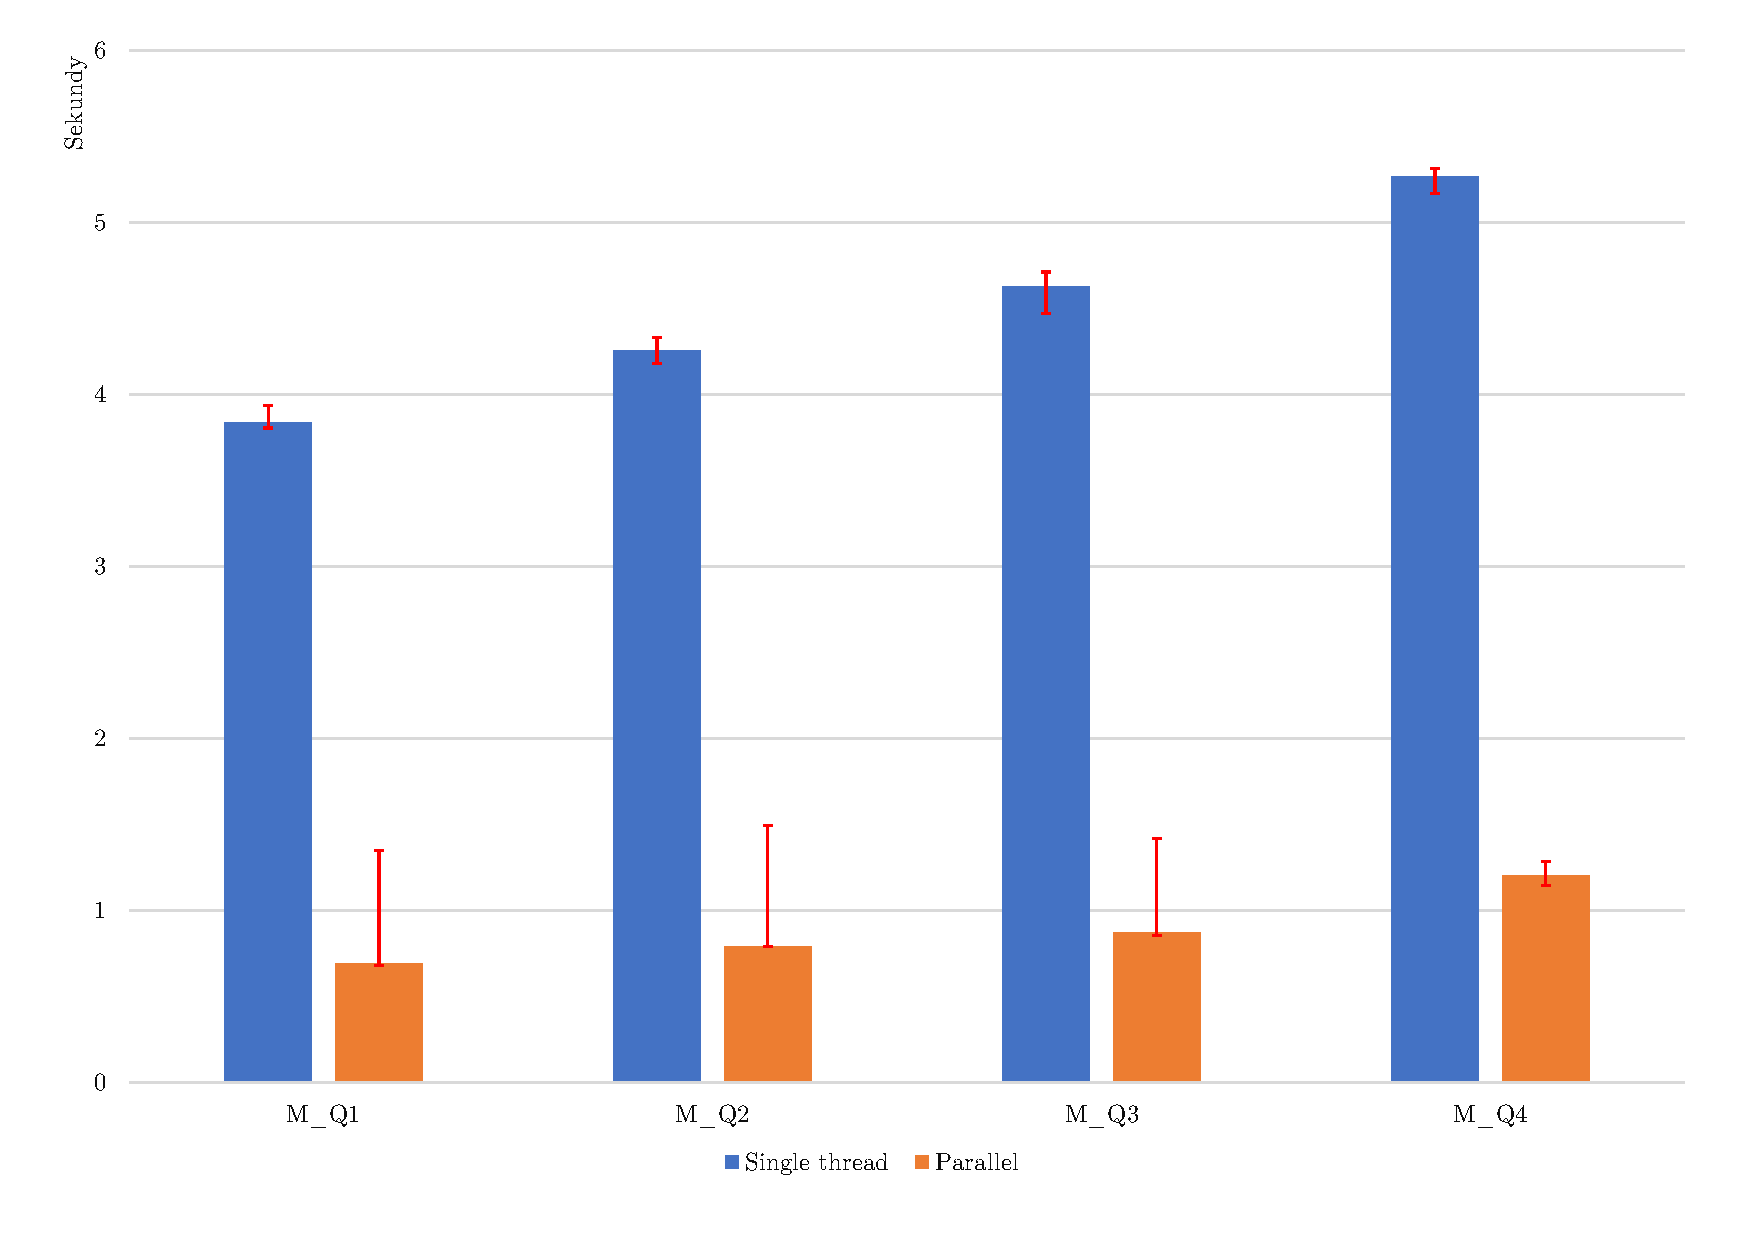
\includegraphics[width=\linewidth]{../img/amazonMatch.pdf}\centering
\caption{Doba vykonání dotazů Match pro graf Amazon0601 (sekce \ref{tab.grafBase}). Jedno vlákno vůči osmi vláknům.}
\label{figure.amazonMatch}
\end{figure}

\begin{figure}[!htp]
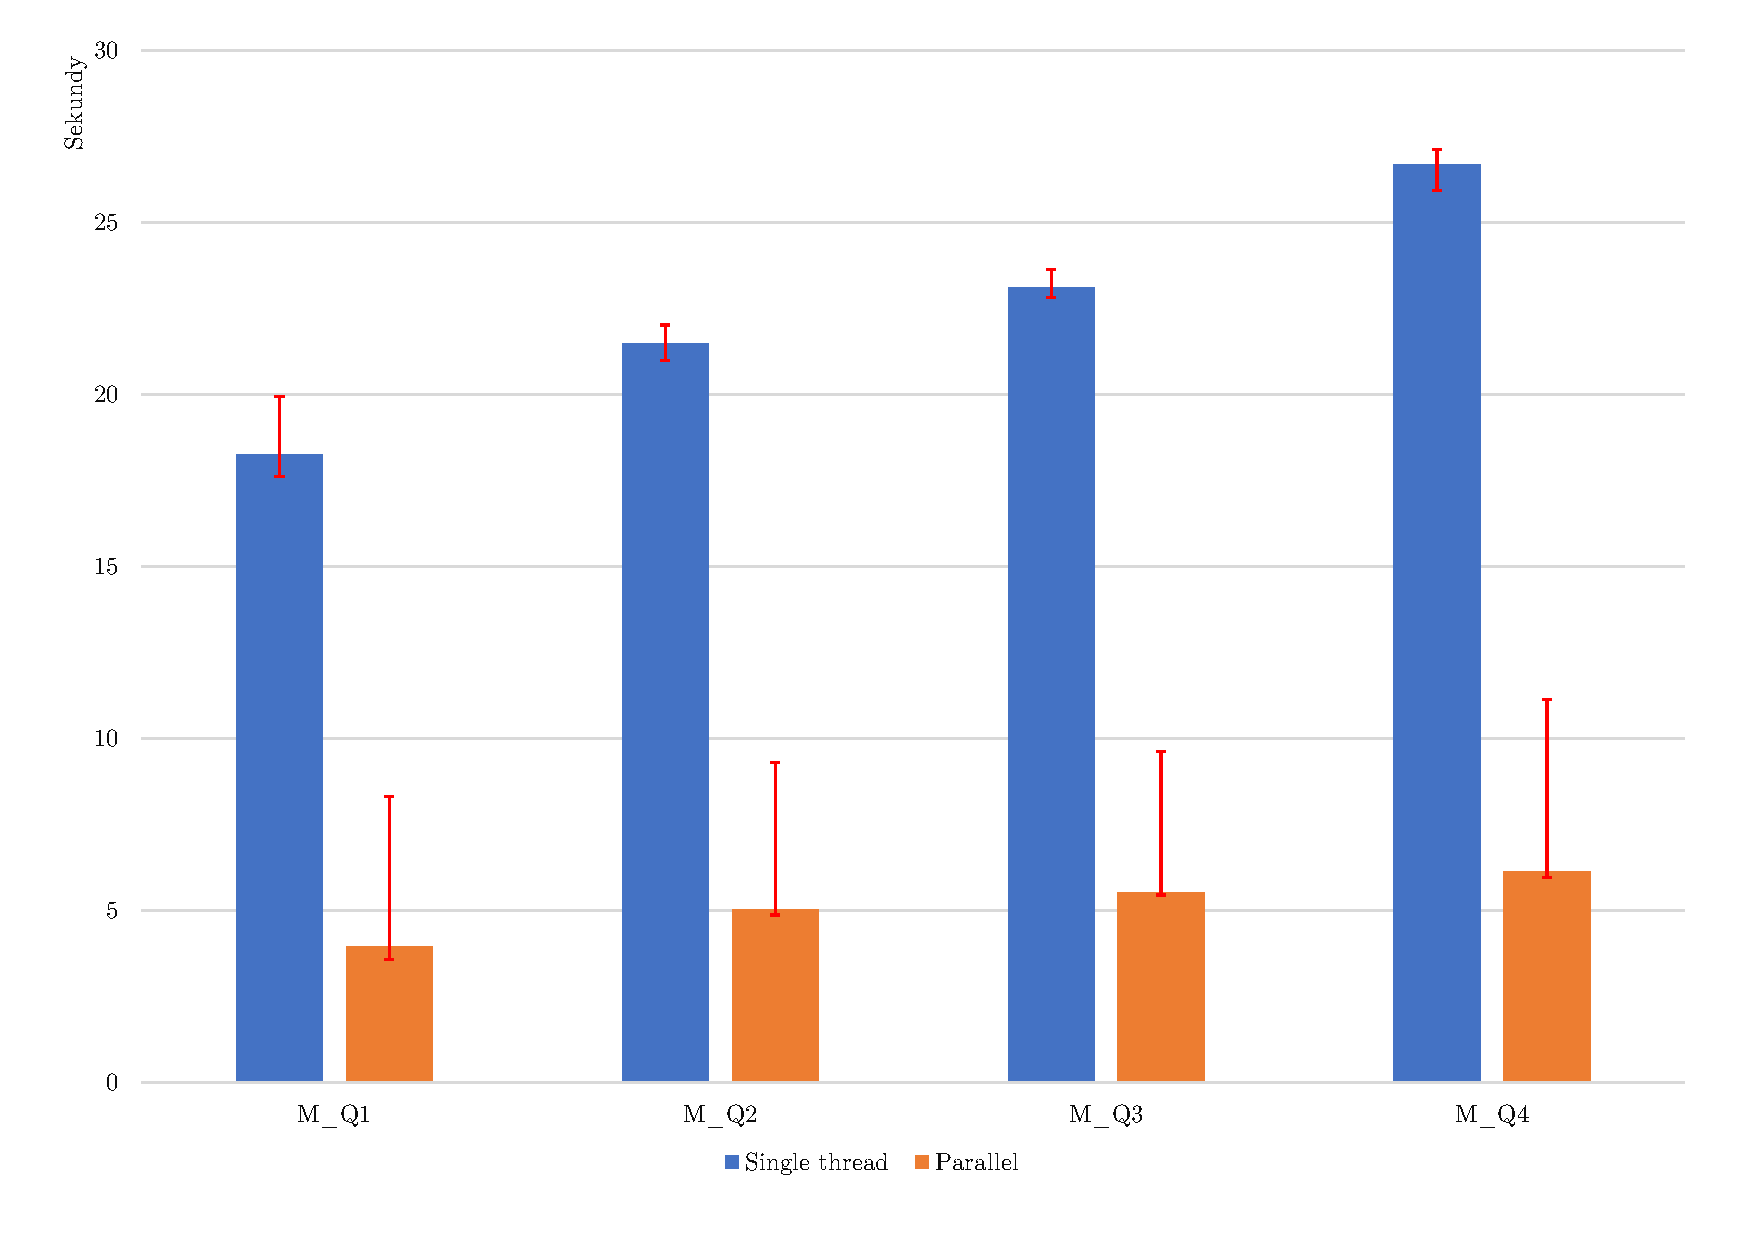
\includegraphics[width=\linewidth]{../img/webberkstanMatch.pdf}\centering
\caption{Doba vykonání dotazů Match pro graf WebBerkStan (sekce \ref{tab.grafBase}). Jedno vlákno vůči osmi vláknům}
\label{figure.webberkstanMatch}
\end{figure}

\begin{figure}[!htp]
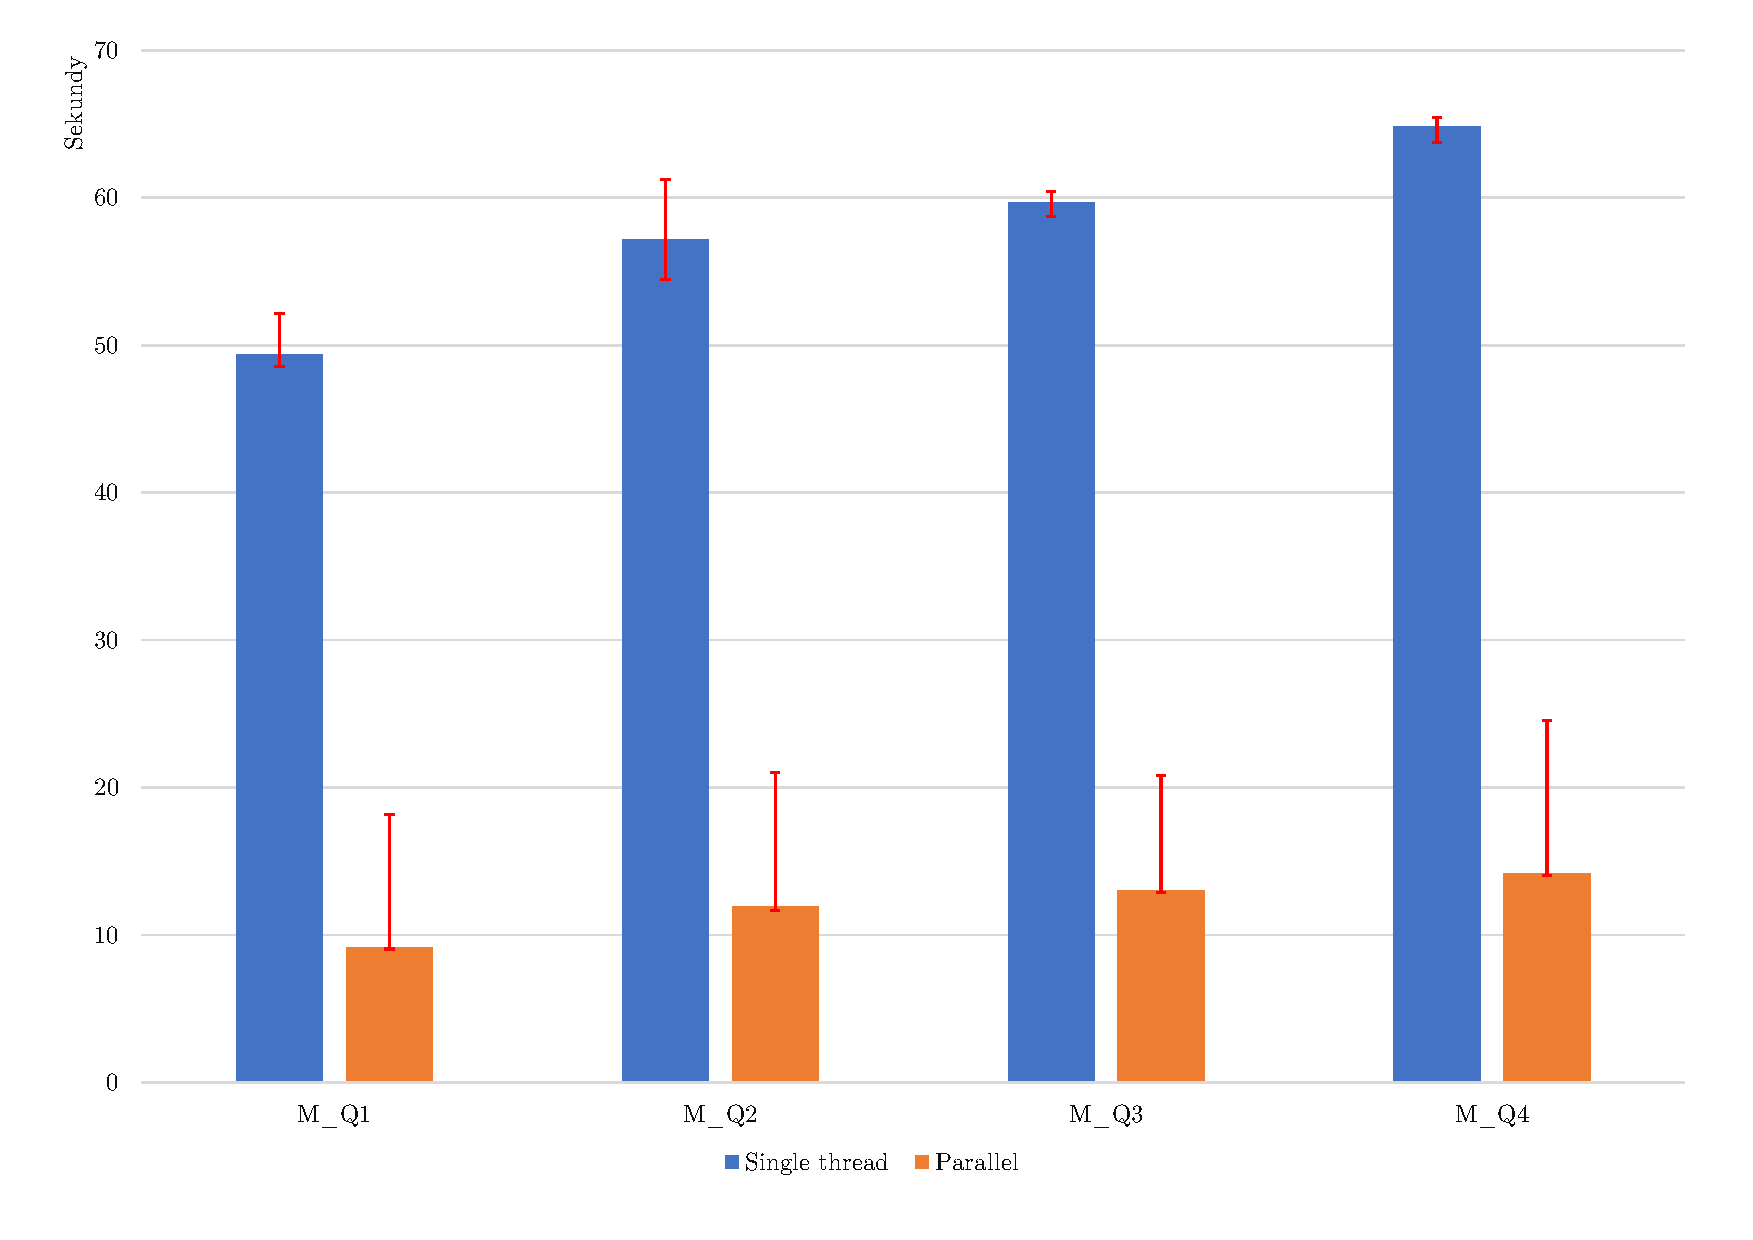
\includegraphics[width=\linewidth]{../img/skitterMatch.pdf}\centering
\caption{Doba vykonání dotazů Match pro graf As-Skitter (sekce \ref{tab.grafBase}). Jedno vlákno vůči osmi vláknům.}
\label{figure.skitterMatch}
\end{figure}


\subsection{Order by}

Z důvodu časové a prostorové složitosti třídění na grafu As-Skitter jsme se rozhodli jej vynechat pro Order by dotazy.
Všechny výsledky měření třídění jsou zobrazeny na obrázcích na konci této sekce.

\subsubsection{Obecné shrnutí jednovláknových řešení}

Nejprve shrneme základní koncepty použitých řešení.
Každé řešení pracuje s tabulkou výsledků, kterou musí setřídit.
Nikdy netřídíme samotné řádky tabulky, ale pouze indexy řádků.
Výsledek třídění je indexační struktura nad tabulkou.
Při porovnávání je nutné mít na paměti, že jednovláknově bežící části používájí cachování popsané v sekcích \ref{anal.orderby.opt1}, \ref{anal.orderby.opt2} a \ref{impl.orderby.opts}.  

Mód \textbf{Normal} využívá k třídění algoritmus Merge sort.
Algoritmus je implementován v knihovně HPCsharp \citep{hpcsharp}.
Třídění probíhá po dokončení prohledávání grafu a třídí celou tabulku výsledků pomocí pole indexů.

Vylepšená řešení zpracovávájí vyhledané výsledky v moment jejich nalezení.
Nalezený prvek se nejdříve vloží do tabulky na nový řádek. 
Následně se index daného řádku vloží do indexační struktury. 
Jako indexační strukturu nad tabulkou používáme $(a, b)$-strom \citep[str. 190]{labyrint}, u kterého jsme upravili definici na $b=2a$.
V našem případě $b=256$.
V řešení \textbf{ABTree} se jedná o obecný $(a, b)$-strom, zatímco řešení \textbf{ABTreeValueAccumulator} výsledky (indexy) mající stejnou hodnotu klíčů třídění, jako již vložené prvky, uloží do \verb+List<int>+.
Tedy místo vytvoření nového záznamu ve stromě dojde pouze k vložení do patřičného pole.

\subsubsection{Výsledky jednovláknového zpracování}

Začneme řešením běžícím v jednom vlákně, tj. grafy  \ref{figure.amazonOrderST} a \ref{figure.webberkstanOrderST}.
Můžeme si všimnout, že výsledky vypadají v rámci daných grafů konzistentně pro každý dotaz.
Ani jedno z vylepšených řešení nedokázalo porazit mód \textbf{Normal}, což odpovídá našim předpokladům. 
Je to způsobeno značnou režií za metodu vložení (\verb+Insert+) do stromu, kdy dochází k častému alokování nových vrcholů a překopírovávání prvků při splitu.
Nejproblematičtější část je množství tříděných výsledků, kdy počet samotných hodnot klíčů třídění je omezen počtem vrcholů v grafu (tabulka \ref{tab.grafBase}). 
Daná situace vede k opakovanému zatřizování výsledků se stejnou hodnotou a tím navyšování velikosti stromu společně s počtem porovnání na \verb+Insert+.
Celý problém jsme vyřešelili v řešení \textbf{ABTreeValueAccumulator}, ve kterém se duplicitní hodnoty ukládají do zmíněného pole a tím omezujeme velikost výsledného stromu. 
Jak vidíme na obrázcích, řešení se přibližuje rychlosti řešení \textbf{Normal}.
Problém by nastal v případě, pokud by množství hodnot odpovídalo počtu nalezených výsledků. 
V tomto případě bychom zbytečně navyšovali režii za vzniklá pole, která se nevyužijí.

\subsubsection{Třídění pomocí vlastnosti vůči \texttt{ID}}

Dle našich předpokladů se ukázalo, že třídění pomocí vlastnosti (O\_Q3 a O\_Q4) vůči \verb+ID+ (O\_Q1 a O\_Q2) vede ke znatelnému zpomalení.
Je to způsobeno nutným přístupem k databázi, při kterém se ověřuje, jestli daná vlastnost existuje na daném elementu a následném čtení hodnoty ze struktury obsahující ji.

\subsubsection{Obecné shrnutí paralelních řešení}

Opět zde platí, že tabulka výsledků je tříděna pomocí indexů.
Mód \textbf{Normal} používá paralelní Merge sort \citep{hpcsharp}.

Vylepšená paralelní zpracování aplikují použité verze $(a, b)$-stromů ze zpracování pro jedno vlákno. 
Každé běžící vlákno v \textbf{Half-Streamed} řešení obsahuje lokální tabulku a indexační strom. 
Po dokončení vyhledávání se obsahy stromů překopírují do pole a dojde k paralelnímu dvoucestnému slévání používající stejnou funkci jako paralelní Merge sort. 
U \textbf{Streamed} řešení jsme navrhli sdílenou strukturu pro zatřizování výsledků.
Struktura rozdělí rozsah hodnot prvního klíče třídění na rovnoměrné části (konkrétněji v sekci \ref{anal.improvement.orderby.streamed})
Počet částí je heuristicky zvolen jako $m=t^2$, kde $t=\#vláken$. 
Pro každou část rozsahu vytvoříme přihrádku obsahující zámek, tabulku a indexační strom.
Při příchozím výsledku se získá hodnota prvního klíče třídění a určí se jeho patřičná přihrádka. 
Do přihrádky vlákno přistoupí pomocí přiloženého zámku.
Následně výsledek vloží do tabulky a index nového řádku tabulky do stromu.
Rozdíl v řešeních je pak jen využitá stromová struktura.
Při porovnávání je nutné mít na paměti, že lokálně bežící části používájí cachování popsané v sekcích \ref{anal.orderby.opt1}, \ref{anal.orderby.opt2} a \ref{impl.orderby.opts}.  

\subsubsection{Výsledky paralelního zpracování}

Nyní budeme prezetovat výsledky paralelizace (obrázky \ref{figure.amazonOrderPar} a \ref{figure.webberkstanOrderPar}).
Na první pohled jsme si všimli mnohonásobného zpomalení \textbf{Streamed} řešení pro dotazy O\_Q1 a O\_Q2.
Výše jsme zmínili základní princip \textbf{Streamed} řešení.
Rozsah hodnot prvního klíče třídění se rozdělí na rovnoměrné části a pro každý takový rozsah existuje přihrádka přístupná pomocí zámku.
Vlákno v moment nalezení výsledku přistupuje k přihrádce pomocí zámku a vloží do ní daný výsledek.
Při implementaci řešení jsme se omezili pouze na celý rozsah hodnot C\# (.NET Framework 4.8) typu vlastnosti.
To znamená, že pokud vlastnost má typ integer (v C\# Int32), ačkoliv hodnoty vlastnosti v grafu mohou být v rozsahu $[0; 100]$, tak rozdělení přihrádek se vytvářejí z celého rozsahu C\# typu.
Tedy přihrádky se vytvářejí rozdělením rozsahu $[$\verb+Int32.MinValue+; \verb+Int32.MaxValue+$]$ a nikoliv $[0; 100]$.
To má za následek při třídění pomocí vlastnosti s rozsahem hodnot v grafu $[0; 100]$, že vlákna budou přistupovat v nejhorším případě k pouze jedné přihrádce.
Vlákna pak budou vždy čekat na úvólnění jednoho zámku.
Přesně tato situace nastala u \textbf{Streamed} řešení pro dotazy O\_Q1 a O\_Q2.
V nich třídíme pomocí vlastnosti \texttt{ID}. 
\texttt{ID} je typu integer.
Vlastnost typu integer je v C\# typ Int32.
Vytvoří se přihrádky rozdělením rozsahu $[$\verb+Int32.MinValue+; \verb+Int32.MaxValue+$]$.
Rozsah se rozdělí na 64 dílů, protože jsme určili počet přihrádek jako $m=t^2$, kde $t=\#vláken$ a všechny testy běži v osmi vláknech.
Ale problém je, že hodnoty \texttt{ID} vrcholů jsou z omezeného rozsahu $[0; \#$vrcholů v grafu$]$, zatímco pouze jedna přihrádka obsahuje posloupnost 67 108 863 hodnot.
A vždy platí, že 67 108 863 $> \# $vrcholů v grafu (z tabulky \ref{tab.grafBase}).
Čili vlákna vždy přistupují pouze k přihrádce, kde se synchronizují pomocí zámku. 
Výsledná doba zpracování pak odpovídá jednovláknovému zpracování s přidanou režií za přístup k zámku.

Naopak u dotazů O\_Q3 a O\_Q4 je tříděno pomocí hodnot vygenerovaných náhodně spadající do celého rozsahu typu klíče a zde \textbf{Streamed} řešení předčilo všechna ostatní. 
Pro budoucí rozšíření by bylo nutné zvážit vytvoření statistik rozsahů jednotlivých vlastností, aby bylo možné lépe vytvořit rozdělení přihrádek.

\subsubsection{Zrychlení paralelních řešení pro O\_Q3 a O\_Q4 }

\textbf{Half-Streamed} řešení se přibližuje \textbf{Normal} řešení v prvních dvou dotazech a překonává jej ve třetím i čtvrtém dotazu pro řešení používající ABTreeValueAccumulator.
U třetího a čtvrtého dotazu se porovnává pomocí vlastností. V jednovláknovém zpracovávání jsme viděli režii za dané porovnání.
V druhém kroku u daného \textbf{Half-Streamed} řešení dochází k slévání pouze akumulovaných skupin, což rapidně sníží počet porovnávání při slévání a odtud výhoda oproti \textbf{Normal: Merge sort} řešení. 
To samé platí u \textbf{Streamed} řešení, protože počáteční rozhašování způsobí vkládání do mnohonásobně menší skupiny výsledků. 
Celá situace je navíc umocněna zmíněným cachovaním porovnávaných hodnot. 

\subsubsection{Rozsah zrychlení paralelních řešení}

Zajímavý výsledek testování je rozsah zrychlení vylepšených módů, tj. tabulky \ref{tab.OrderByZrychleniAmazon} a \ref{tab.OrderByZrychleniWebBerkStan}). 
Zrychlení Merge sortu zaostavá. 
Maximální zrychlení u ostatních řešení je až pětinásobné. 
Danou situaci si vysvětlujeme následovně.
Implementace paralelního algoritmu Merge sort funguje na principu postupného rekurzivního rozdělování, při kterém se vytváří nové \verb+Tasks+ pro \verb+ThreadPool+.
U vylepšených řešení běži jedna metoda pro každé vlákno po dobu celého zpracování. 


\begin{figure}[!htp]
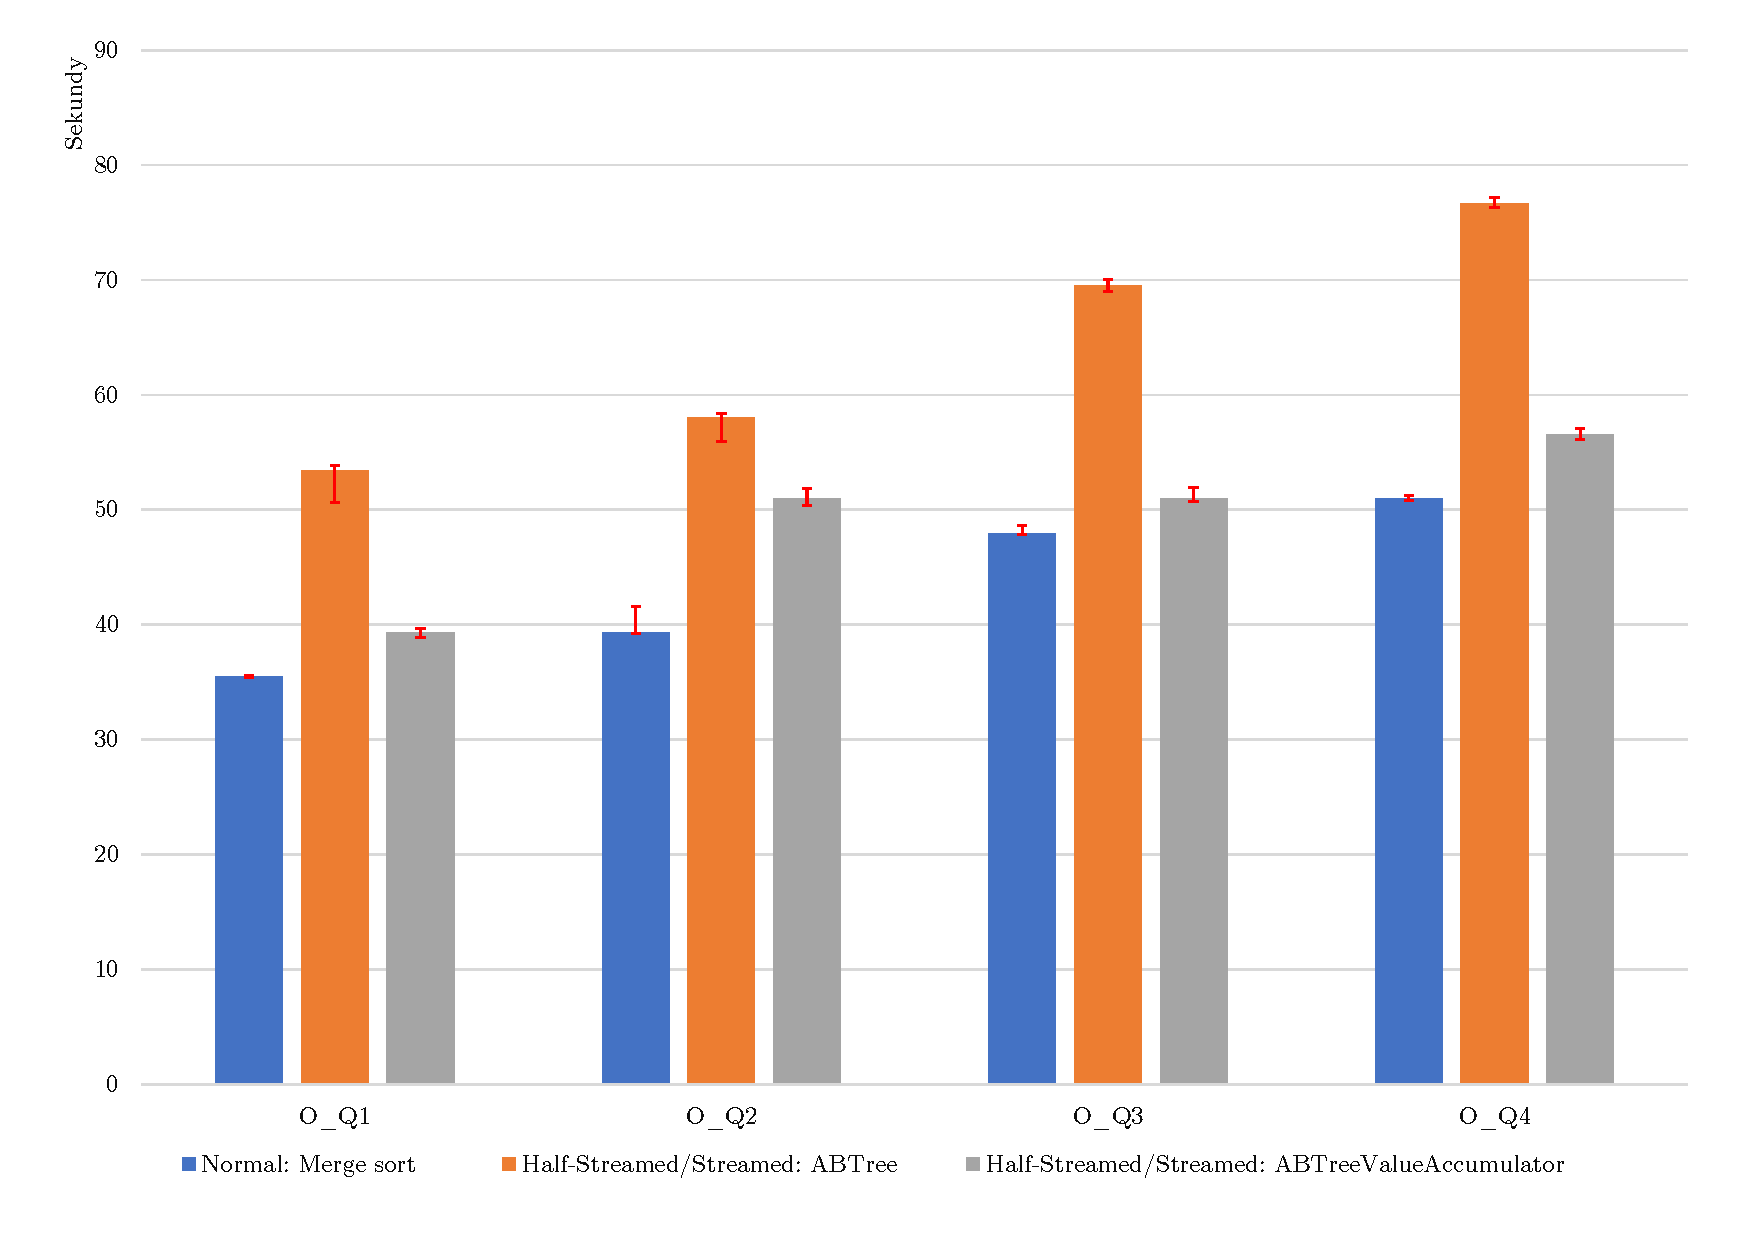
\includegraphics[width=\linewidth]{../img/amazonOrderByST.pdf}\centering
\caption{Doba vykonání dotazů Order by pro graf Amazon0601 (sekce \ref{tab.grafBase}). Běh v jednom vláknu.}
\label{figure.amazonOrderST}
\end{figure}
\begin{figure}[!htp]
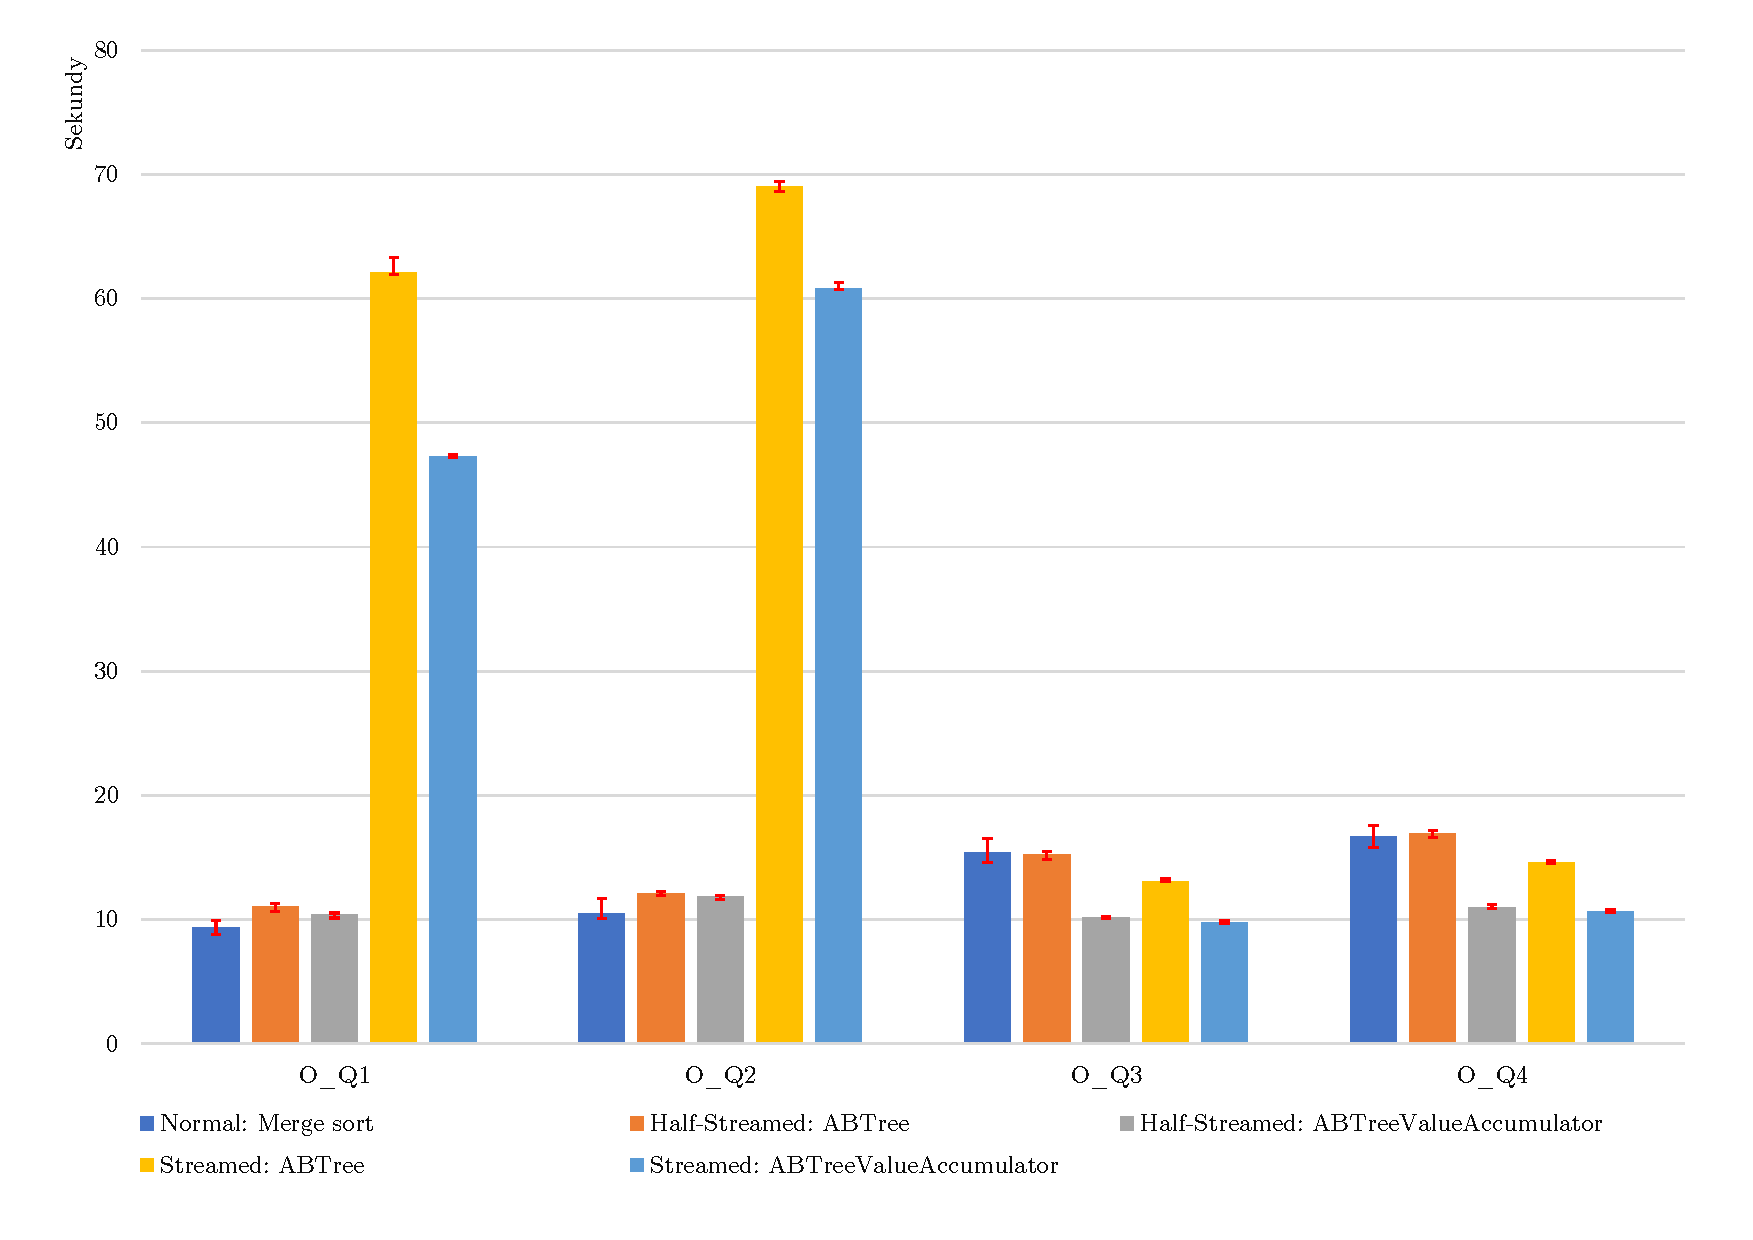
\includegraphics[width=\linewidth]{../img/amazonOrderByPar.pdf}\centering
\caption{Doba vykonání dotazů Order by pro graf Amazon0601 (sekce \ref{tab.grafBase}).  Běh osmi vláken.}
\label{figure.amazonOrderPar}
\end{figure}

\begin{figure}[!htp]
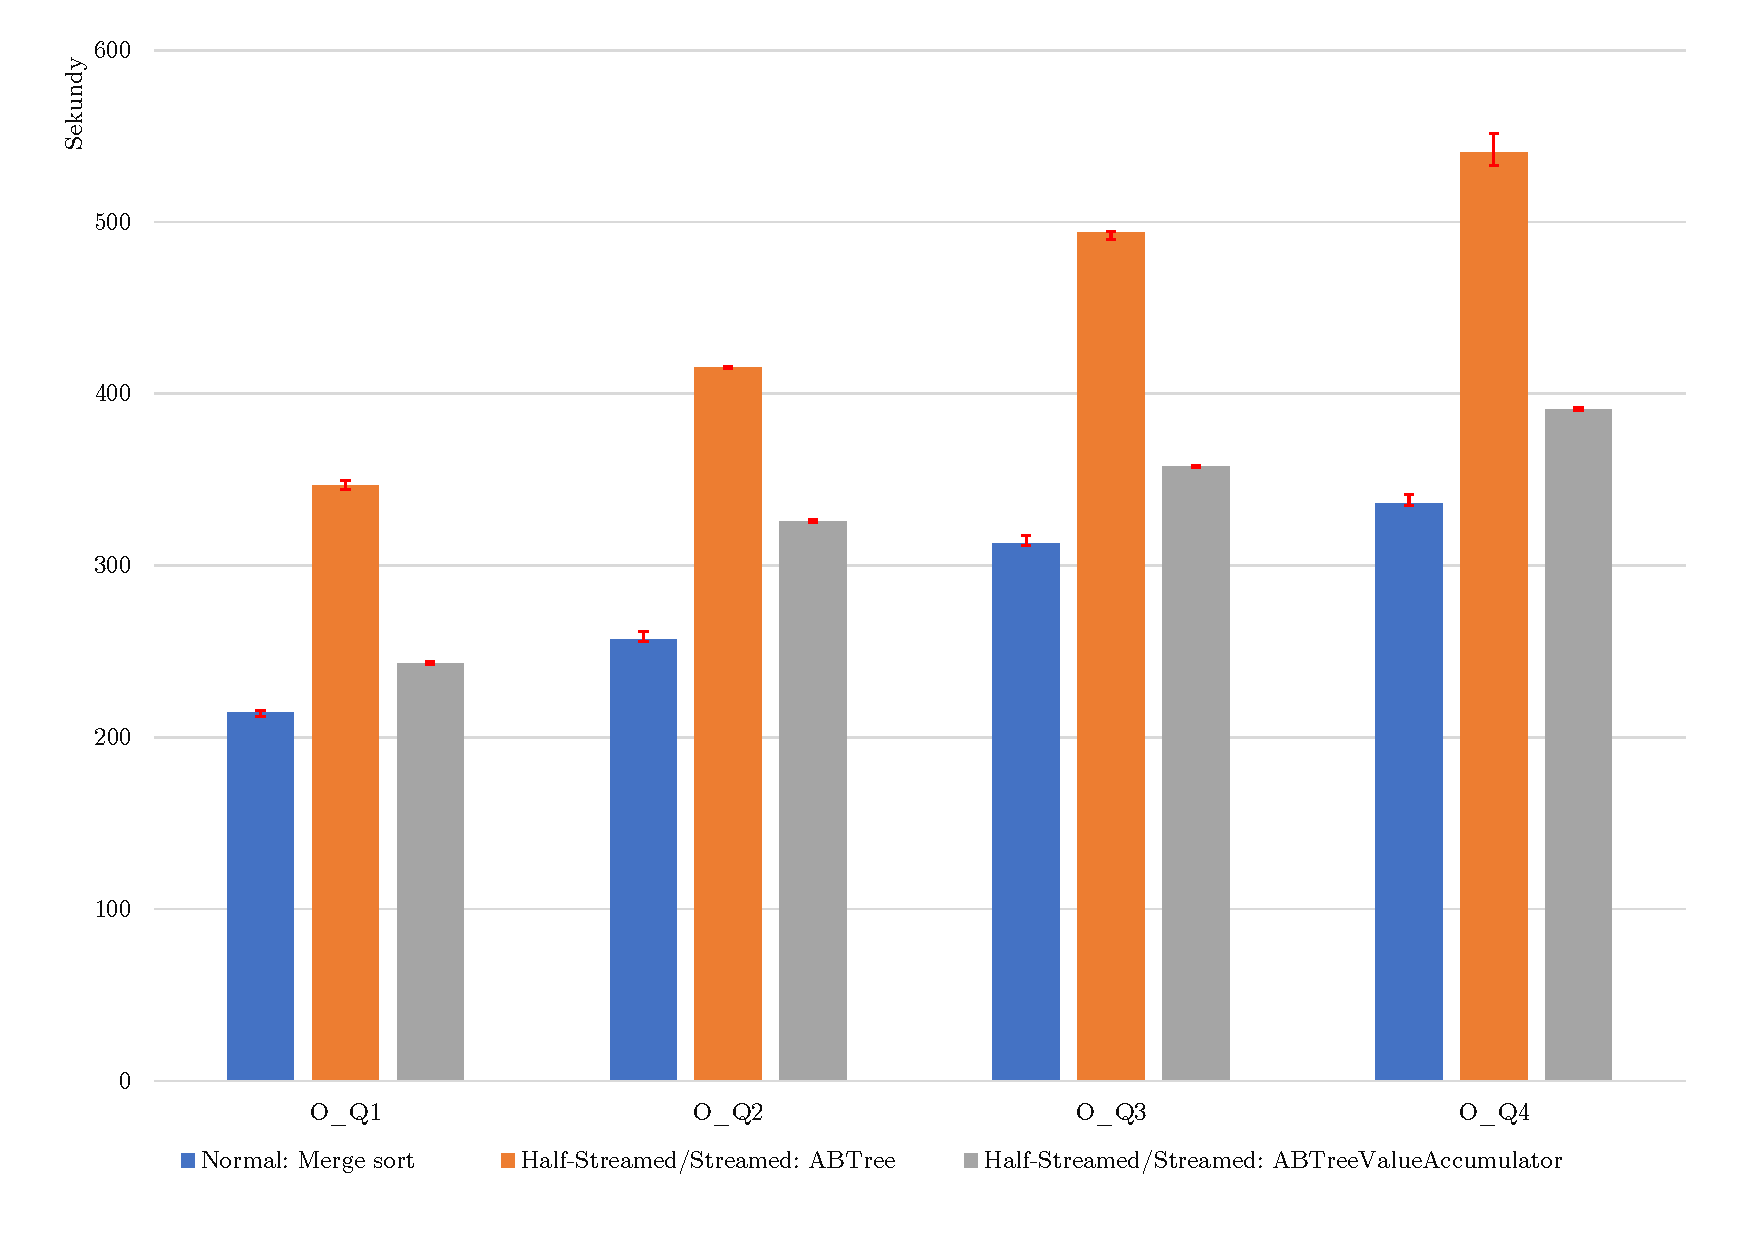
\includegraphics[width=\linewidth]{../img/webberkstanOrderByST.pdf}\centering
\caption{Doba vykonání dotazů Order by pro graf WebBerkStan (sekce \ref{tab.grafBase}). Běh v jednom vláknu.}
\label{figure.webberkstanOrderST}
\end{figure}
\begin{figure}[!htp]
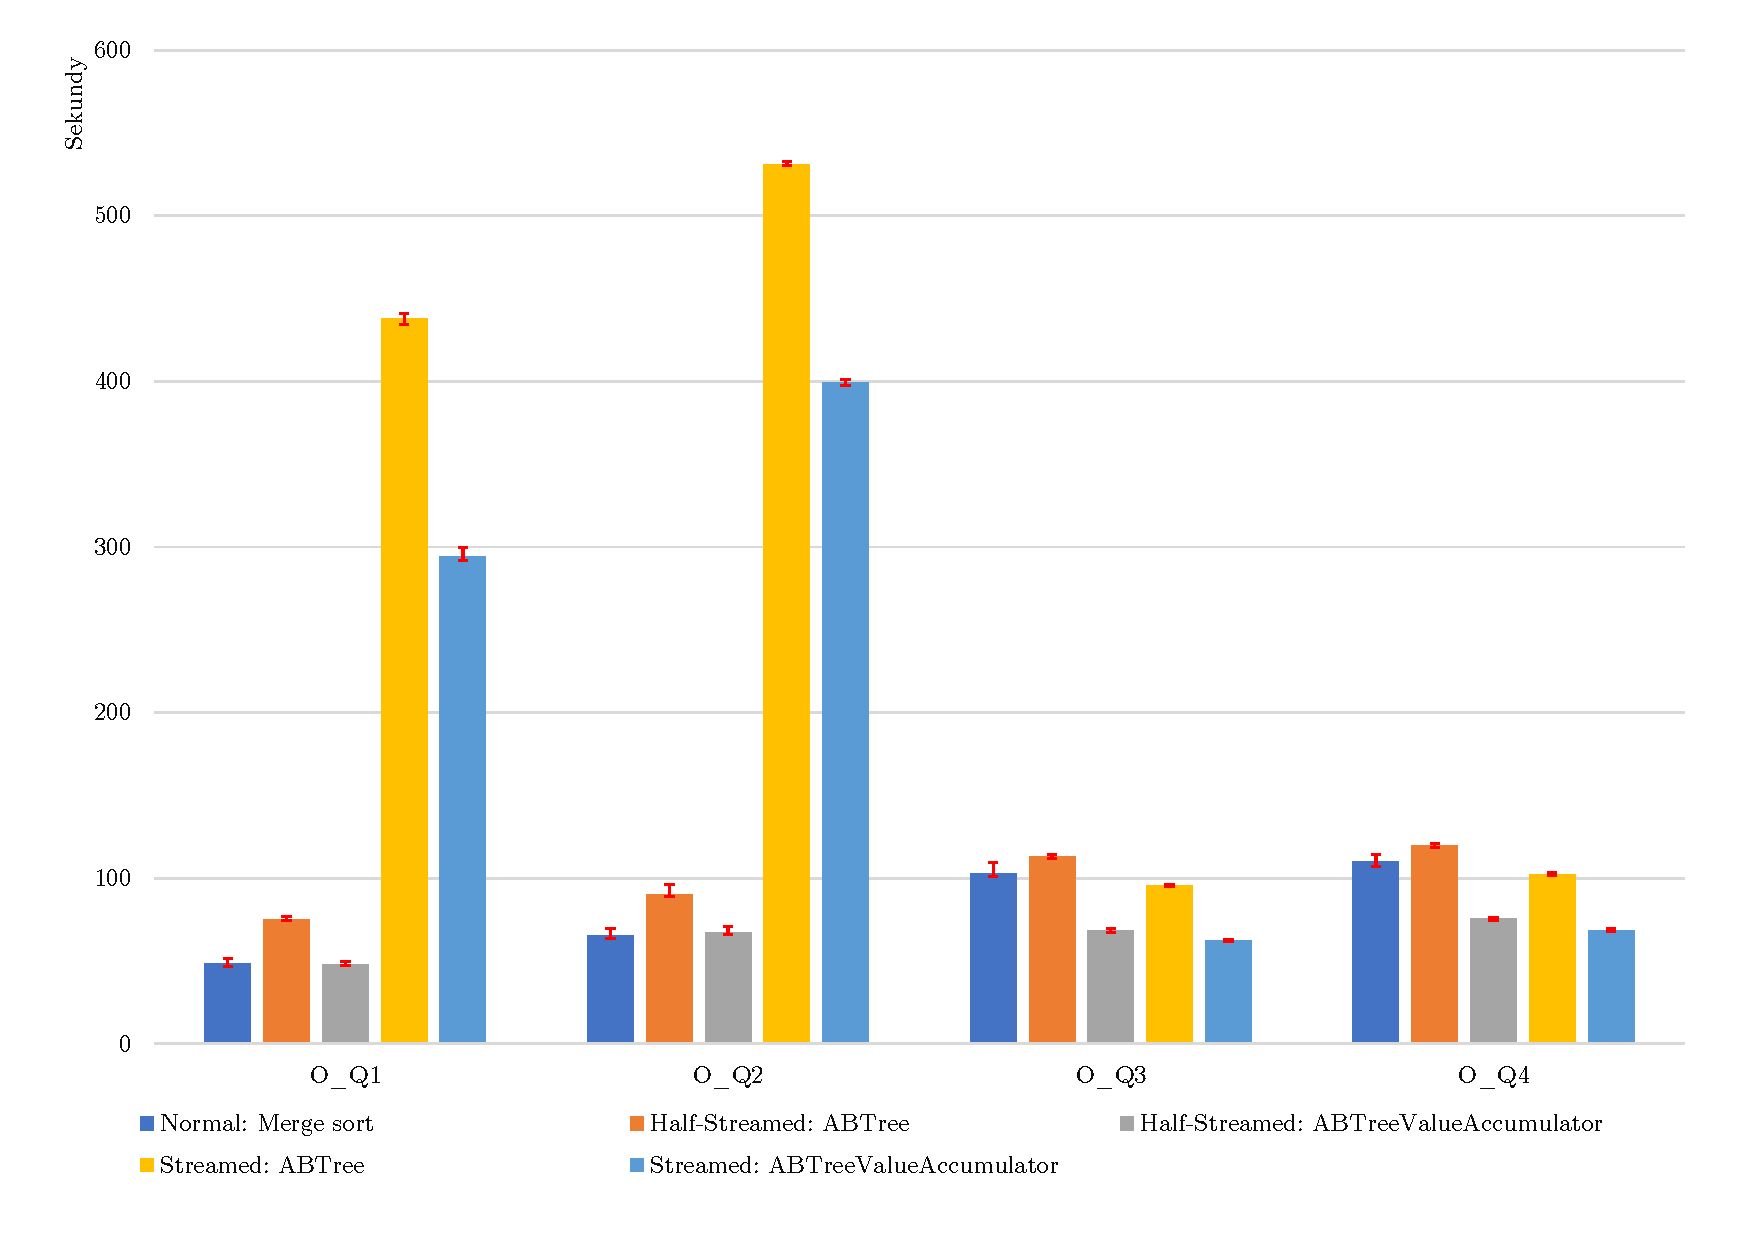
\includegraphics[width=\linewidth]{../img/webberkstanOrderByPar.pdf}\centering
\caption{Doba vykonání dotazů Order by pro graf WebBerkStan (sekce \ref{tab.grafBase}).  Běh osmi vláken.}
\label{figure.webberkstanOrderPar}
\end{figure}

\clearpage

\begin{table}[!htb]
\centering
\begin{tabular}{lrrrr}
\toprule
\mc{} & \mc{O\_Q1} & \mc{O\_Q2} & \mc{O\_Q3} & \mc{O\_Q4} \\
\midrule
Normal: Merge sort                              & 3,79	& 3,75 &	3,12 &	3,05 \\
Half-Streamed: ABTree                   & 4,81	& 4,78 &	4,56 &	4,54 \\
Half-Streamed: ABTreeValueAccumulator   & 3,76	& 4,31 &	5,03 &	5,14 \\
Streamed: ABTree                        & 0,83	& 0,84 &	5,23 &	5,33 \\
Streamed: ABTreeValueAccumulator        & 0,86	& 0,84 &	5,30 &	5,25 \\ 
\bottomrule
\end{tabular}

\caption{Rozsah zrychlení paralelizovaných řešení pomocí osmi vláken pro dotazy Order by nad grafem Amazon0601 (sekce \ref{tab.grafBase}). Tabulka zobrazuje podíl jednovláknového vůči paralelnímu zpracování.}
\label{tab.OrderByZrychleniAmazon}
\end{table}

\begin{table}[!htb]
\centering
\begin{tabular}{lrrrr}
\toprule
\mc{} & \mc{O\_Q1} & \mc{O\_Q2} & \mc{O\_Q3} & \mc{O\_Q4} \\
\midrule
Normal: Merge sort                              & 4,43	& 3,94	& 3,03 &	3,05 \\
Half-Streamed: ABTree                   & 4,59	& 4,61	& 4,36 &	4,51 \\
Half-Streamed: ABTreeValueAccumulator   & 5,05	& 4,83	& 5,21 &	5,18 \\
Streamed: ABTree                        & 0,83	& 0,82	& 5,72 &	5,72 \\
Streamed: ABTreeValueAccumulator        & 0,79	& 0,78	& 5,15 &	5,29 \\ 
\bottomrule
\end{tabular}

\caption{Rozsah zrychlení paralelizovaných řešení pomocí osmi vláken pro dotazy Order by nad grafem WebBerkStan (sekce \ref{tab.grafBase}). Tabulka zobrazuje podíl jednovláknového vůči paralelnímu zpracování.}
\label{tab.OrderByZrychleniWebBerkStan}
\end{table}


Jako důsledek testování můžeme konstatovat, že třídění v průběhu vyhledávání nepřináší předpokládané výhody.
Zrychlení nastává pouze u paralelizace řešení při dostatečně náhodném rozložení dat třídění, pokud samotná porovnání jsou drahá.
Zmínili jsme, že pro stromy nastává zpomalení kvůli reřii za \texttt{Insert}.
V našich vylepšeních jsme neimplementovali předalokovávání vrcholů stromu.
Jestli by pomocí předalokování nastalo zrychlení, které by předčilo řešení \textbf{Normal}, ponecháme jako budoucí rozšíření. 

\subsection{Group by}

\subsubsection{Obecné shrnutí jednovláknových řešení}

Než postoupíme dál připomeneme hlavní rozdíly řešení a značení u zobrazených grafů. 
Každé řešení používá k Group by mapu (\verb+Dictionary<key, value>+).
\textbf{Normal} řešení ukládá všechny výsledky vyhledávání vzoru do tabulky a po dokončení vykoná Group by. 
\textbf{Half-Streamed} řešení vykonává Group by v průběhu prohledávání a ukládá do tabulky pouze výsledky, pro které ještě neexistuje skupina v použité mapě.
Pro zmíněná řešení se jako \verb+key+ používá index do tabulky a skrze něj se následně vypočtou hodnoty klíče.
\textbf{Streamed} řešení nepoužívá tabulku, ale hodnoty klíče ukládá rovnou do mapy. 
Objevující se značení Bucket a List určuje způsob ukládání výsledků agregačních funkcí (\verb+min+, \verb+avg+...) jako \verb+value+ záznam v mapě.
Podrobnější vysvětlení je v kapitole Analýzy \ref{anal.groupby.uloziste}.
Výsledky jednovláknového seskupování jsou zobrazeny na obrázcích před shrnutím paralelních výsledků seskupování v sekci \ref{expr.results.groupby.par}.

\subsubsection{Výsledky jednovláknového zpracování}

Na obrázcích \ref{figure.amazonGroupByST}, \ref{figure.webberkstanGroupByST} a \ref{figure.skitterGroupByST} vidíme výsledky Group by pro běh v jednom vlákně.
Výsledky na obrázcích \ref{figure.amazonGroupBySTNoAgg}, \ref{figure.webberkstanGroupBySTNoAgg} a \ref{figure.skitterGroupBySTNoAgg} představují dotazy bez agregačních funkcí v části Select.
Dvojice G\_Q4/G\_Q5, G\_Q2/G\_Q3 a trojice G\_Q6/G\_Q7/G\_Q8 dotazů jsou pouze mírně rozličné a můžeme u nich vidět konzistenci výsledků pro použité grafy.
Řešení vykonávající Group by v průběhu vyhledávání překonávají \textbf{Normal} řešení.
S růstem počtu výsledku se rozdíly mezi módy prohlubují. 
Například, zrychlení \textbf{Streamed} řešení je znatelnější u grafu As-Skitter než u grafu Amazon0601. 
Obecně nejznačnější zrychlení nastává u \textbf{Streamed} řešení, kdy není použita tabulka výsledků.

\subsubsection{Zpomalení jednovláknového Half-Streamed řešení}

Velice mírné zrychlení můžeme vidět u \textbf{Half-Streamed} řešení, které ukládá jen reprezentanty skupiny.
U všech dotazů bez agregačních funkcí, kromě dvojice G\_Q4$'$/G\_Q5$'$, nastávají situace, kdy \textbf{Half-Streamed} řešení je pomalejší než \textbf{Normal}.
U grafu Amazon0601 nastává stejná situace pro G\_Q3, G\_Q6 a pro každý graf G\_Q8.
Situaci jsme neočekávali a vysvětlujeme si ji následovně.
\textbf{Half-Streamed} řešení používá při zpracování výsledku položku tabulky \verb+temporaryRow+, do které přesouvá ukazatel na pole výsledků.
Skrze danou položku pak následně přistupuje k výsledku při vkládání do mapy. 
Na dané přesouvání se můžeme dívat jako na kopírovaní jedné proměnné do tabulky.
Při úspěšném vložení nastane navíc překopírování výsledků do pravé tabulky.
Což odpovídá větší režii na zpracování výsledku než u \textbf{Normal} řešení.
Proto vídíme pokles rychlosti a celkově jen mírné zrychlení u \textbf{Half-Streamed} řešení v jiných případech.
Největší skok pak právě nastává v dotazech G\_Q4/G\_Q4$'$ a G\_Q5/G\_Q5$'$, kdy se ukládají dvě proměnné.
Tedy samotná řežie \textbf{Normal} řešení je značně pomalejší, protože musí ukládat vždy dvě proměnné, zatímco \textbf{Half-Streamed} jen přesouvá ukazatel.
Zajímavé je, že dané situace nastávají u dotazů bez agregačních funkcí, přestože všechna řešení pro jejich reprezentaci používají stejné funkce a struktury (List/Bucket).
Předpokládali bychom tedy stejnou situaci i na ostatních (větších) grafech.
Absenci jevu neumíme plně objasnit.

\subsubsection{Porovnání výsledků úložišť List/Bucket jednovláknového zpracování}

Na největším grafu platí, že použité ukládání List je pomalejší než Bucket, kvůli indirekci navíc.
Na menších grafech rozdíly ustupují a dokonce nastavají situace, kdy je List rychlejší. 
Přesněji u dotazů G\_Q4 a G\_Q5.
Přehození rolí si u nich vysvětlujeme režií za množství vytvářených polí (tj. hodně alokací, málo přístupů), které se vyrovná použité indirekci.
Na grafu Amazon0601 u  G\_Q4 a G\_Q5 dotazů je \textbf{Streamed} řešení pomalejší než \textbf{Half-Streamed} s úložištěm List, protože také vytváří pole jako Bucket řešení (viz implementace \ref{impl.improvement.groupby.streamed}).
U dalších grafů je pak počet vytvářených polí mnohonosábně menší než počet přístupů k nim.

\bigskip
Z výsledků můžeme vyvodit, že vylepšená jednovláknová \textbf{Streamed} řešení Group by jsou výhodnější z hlediska rychlosti vykonávání než řešení \textbf{Normal}. 
Nyní přejdeme k výsledkům paralelizace.

\begin{figure}[!htp]
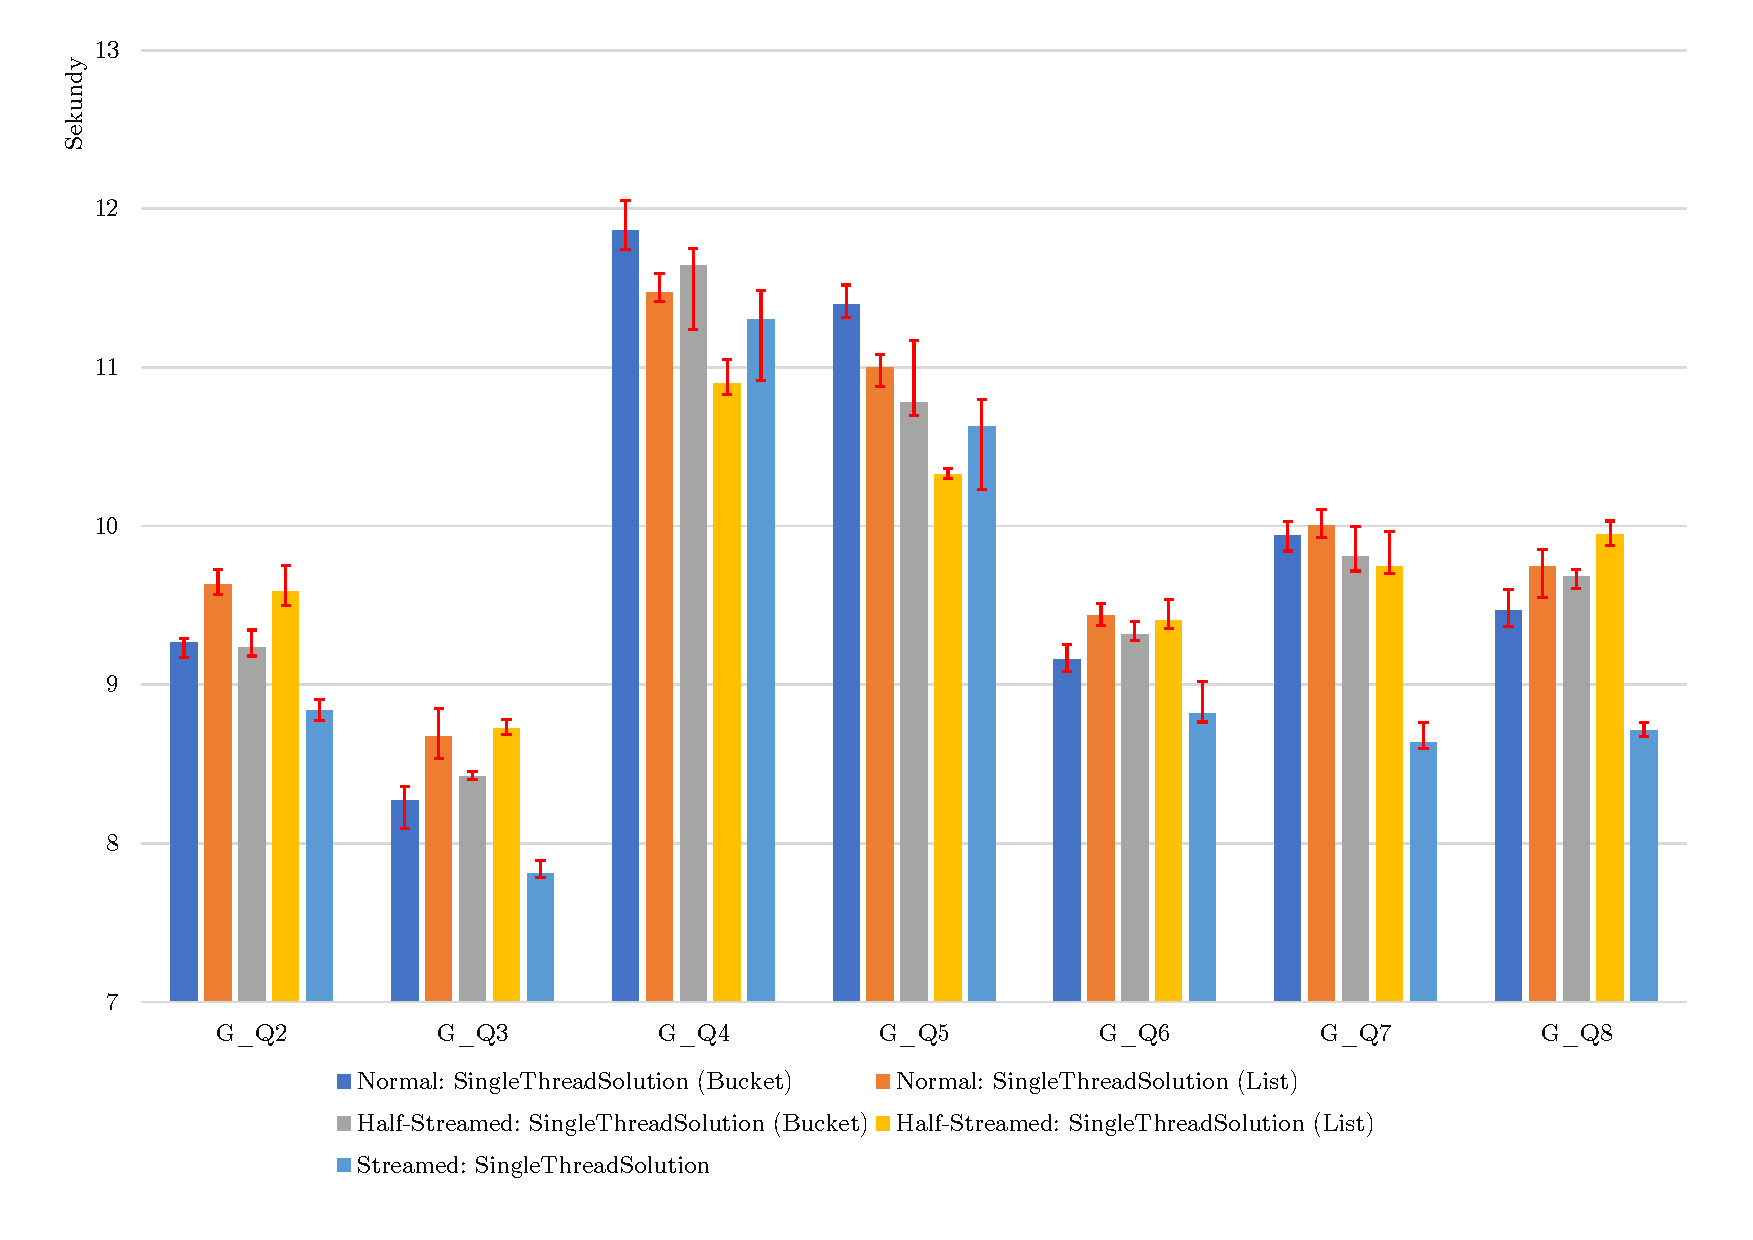
\includegraphics[width=\linewidth]{../img/amazonGroupByST.pdf}\centering
\caption{Doba vykonání dotazů Group by pro graf Amazon0601 (sekce \ref{tab.grafBase}). Běh v jednom vláknu.}
\label{figure.amazonGroupByST}
\end{figure}
\begin{figure}[!htp]
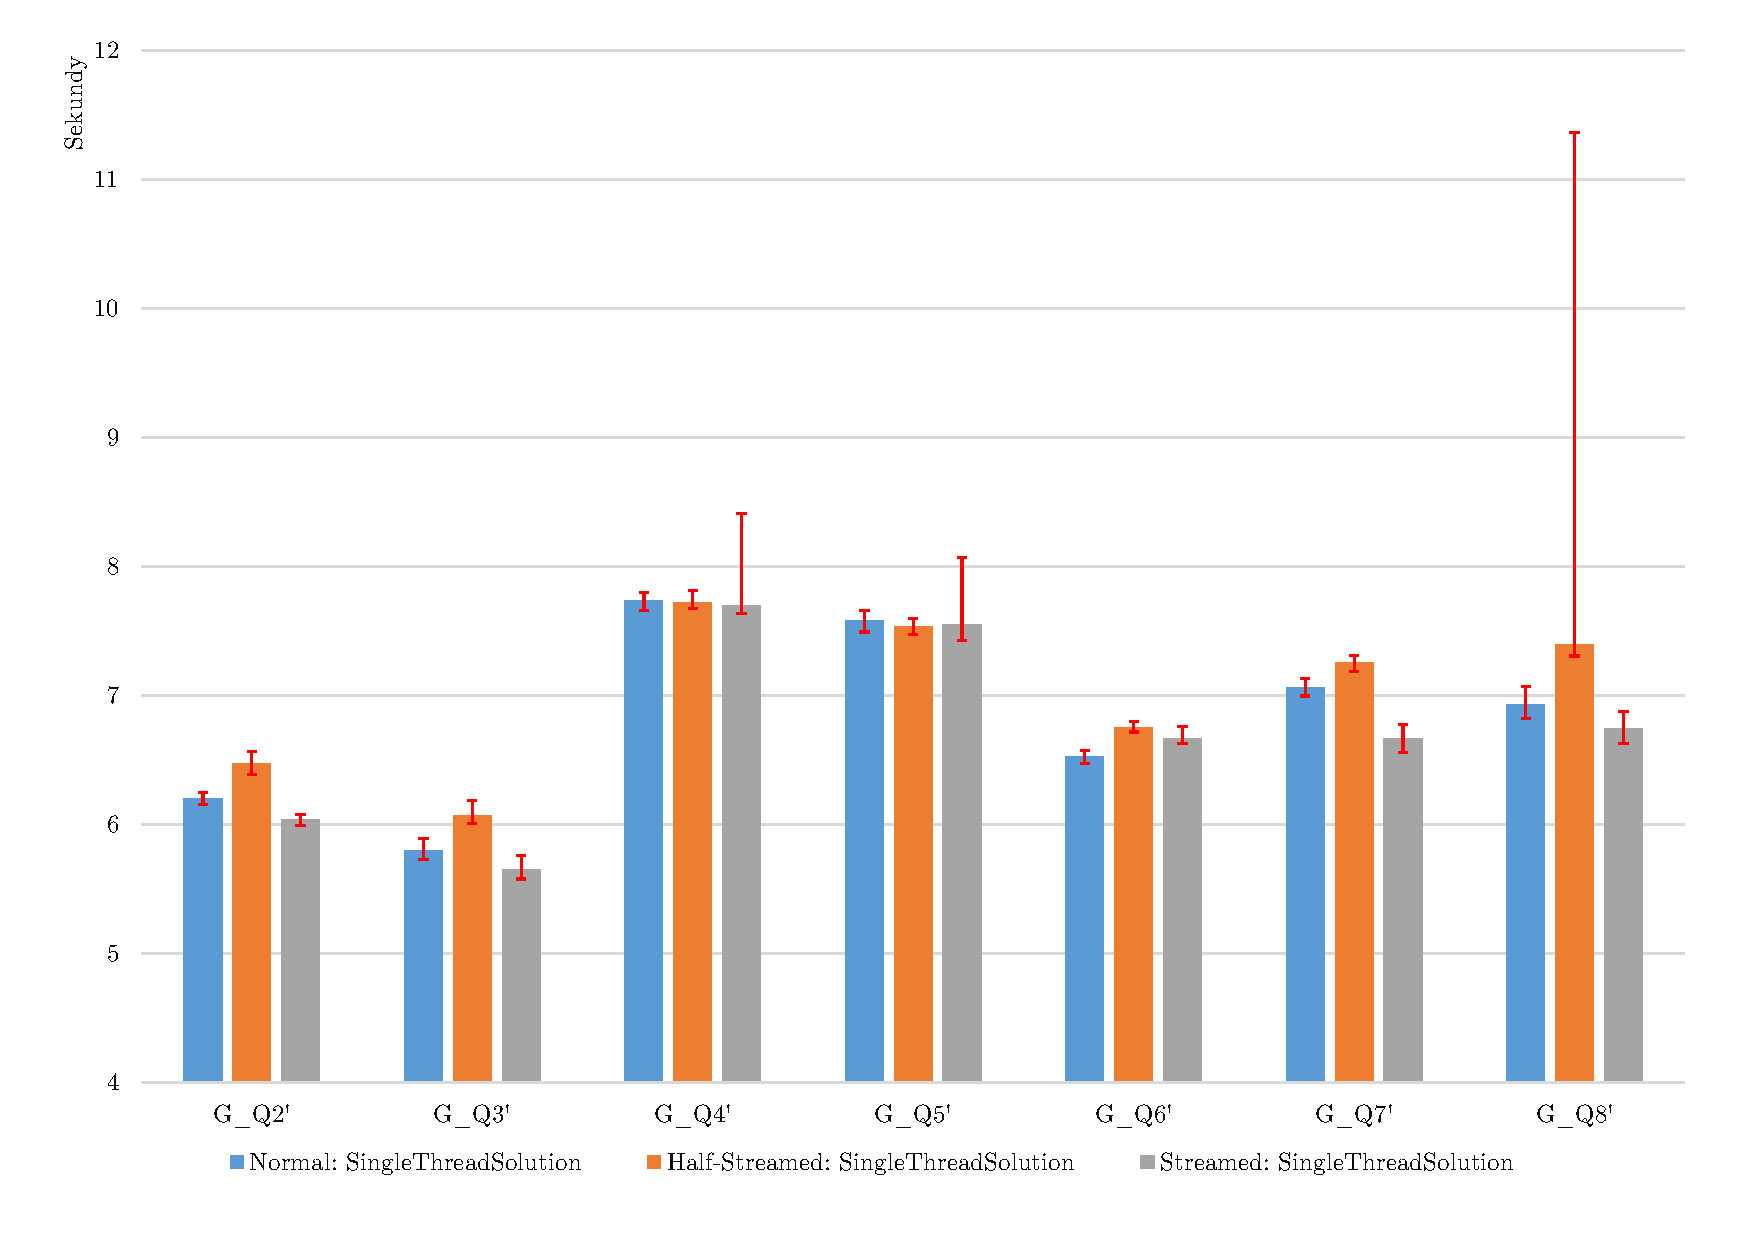
\includegraphics[width=\linewidth]{../img/amazonGroupBySTNoAgg.pdf}\centering
\caption{Doba vykonání dotazů Group by bez agr. funkcí pro graf Amazon0601 (sekce \ref{tab.grafBase}). Běh v jednom vláknu.}
\label{figure.amazonGroupBySTNoAgg}
\end{figure}

\begin{figure}[!htp]
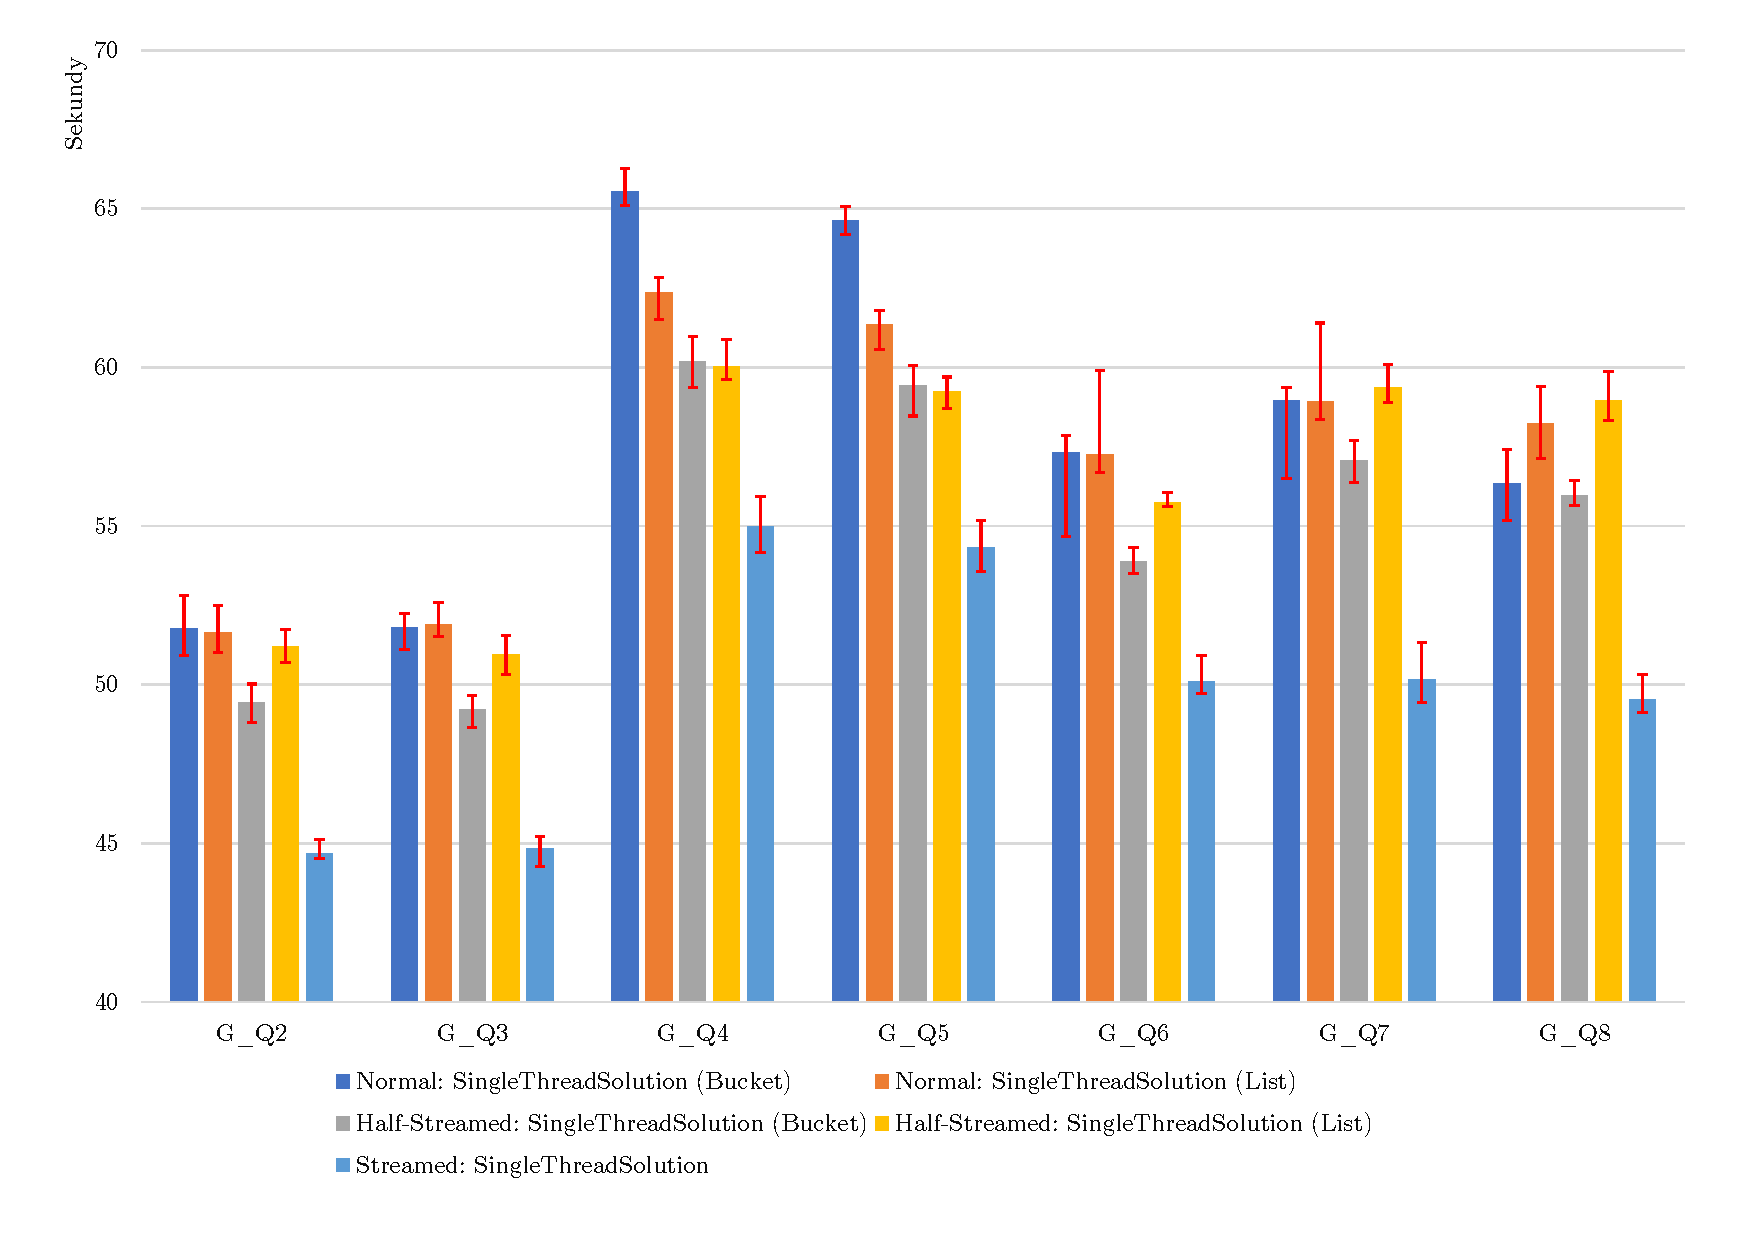
\includegraphics[width=\linewidth]{../img/webberkstanGroupByST.pdf}\centering
\caption{Doba vykonání dotazů Group by pro graf WebBerkStan (sekce \ref{tab.grafBase}). Běh v jednom vláknu.}
\label{figure.webberkstanGroupByST}
\end{figure}
\begin{figure}[!htp]
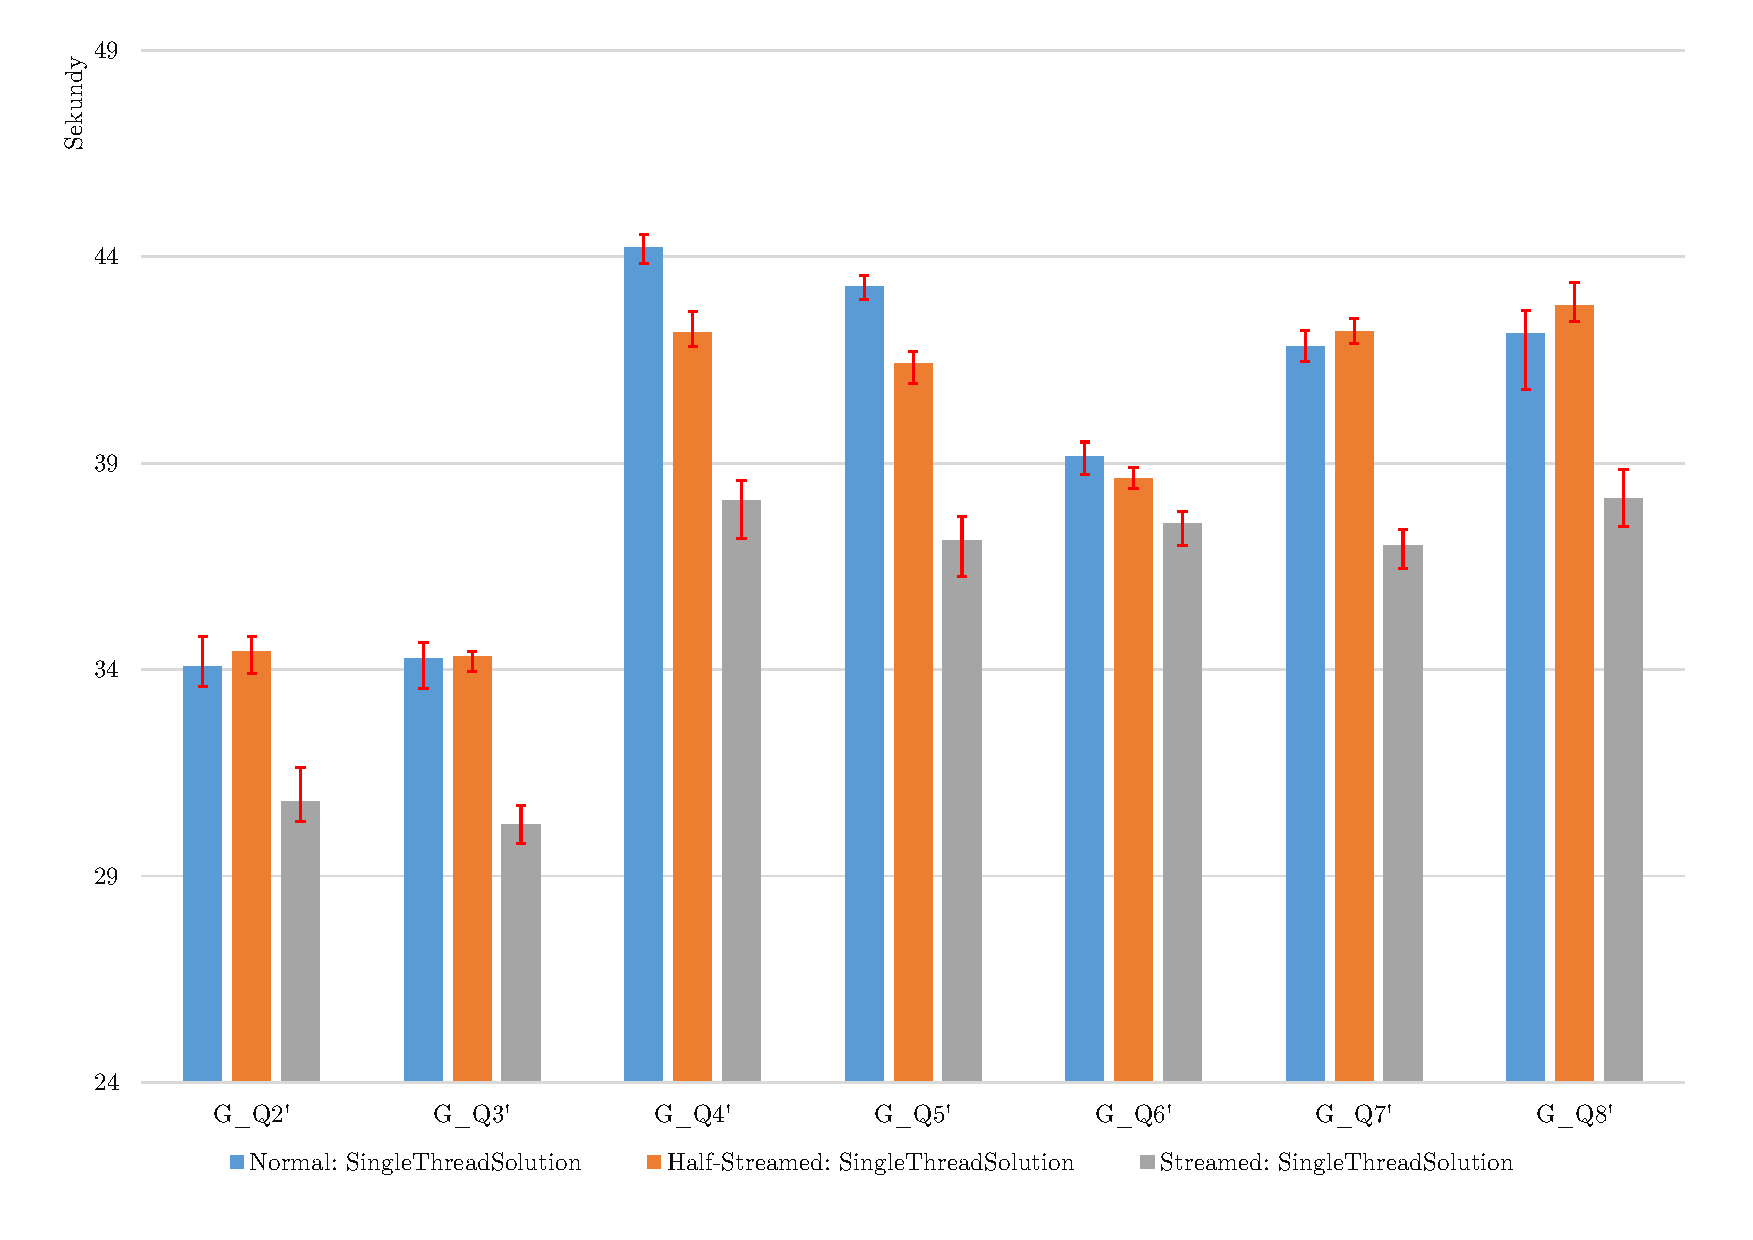
\includegraphics[width=\linewidth]{../img/webberkstanGroupBySTNoAgg.pdf}\centering
\caption{Doba vykonání dotazů Group by bez agr. funkcí pro graf WebBerkStan (sekce \ref{tab.grafBase}). Běh v jednom vláknu.}
\label{figure.webberkstanGroupBySTNoAgg}
\end{figure}

\begin{figure}[!htp]
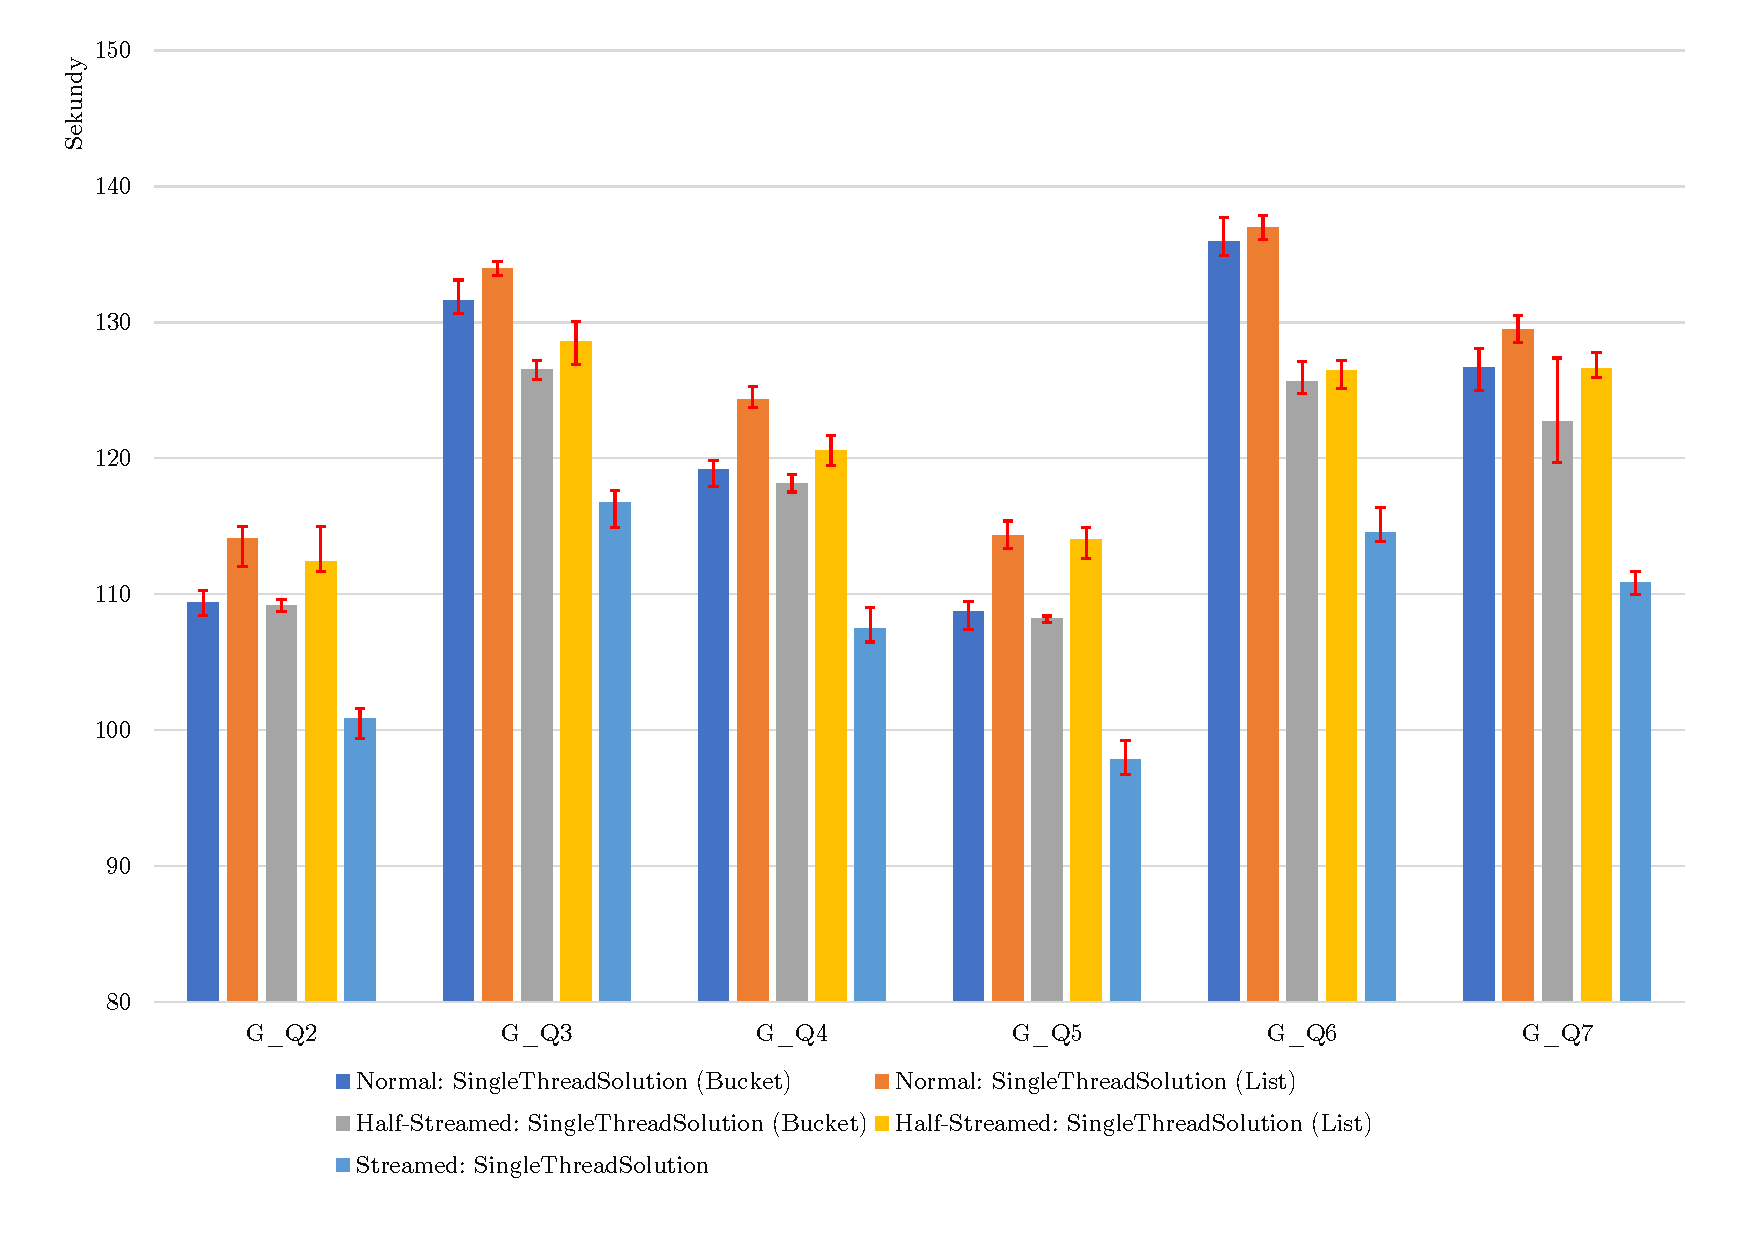
\includegraphics[width=\linewidth]{../img/skitterGroupByST.pdf}\centering
\caption{Doba vykonání dotazů Group by pro graf As-Skitter (sekce \ref{tab.grafBase}). Běh v jednom vláknu.}
\label{figure.skitterGroupByST}
\end{figure}
\begin{figure}[!htp]
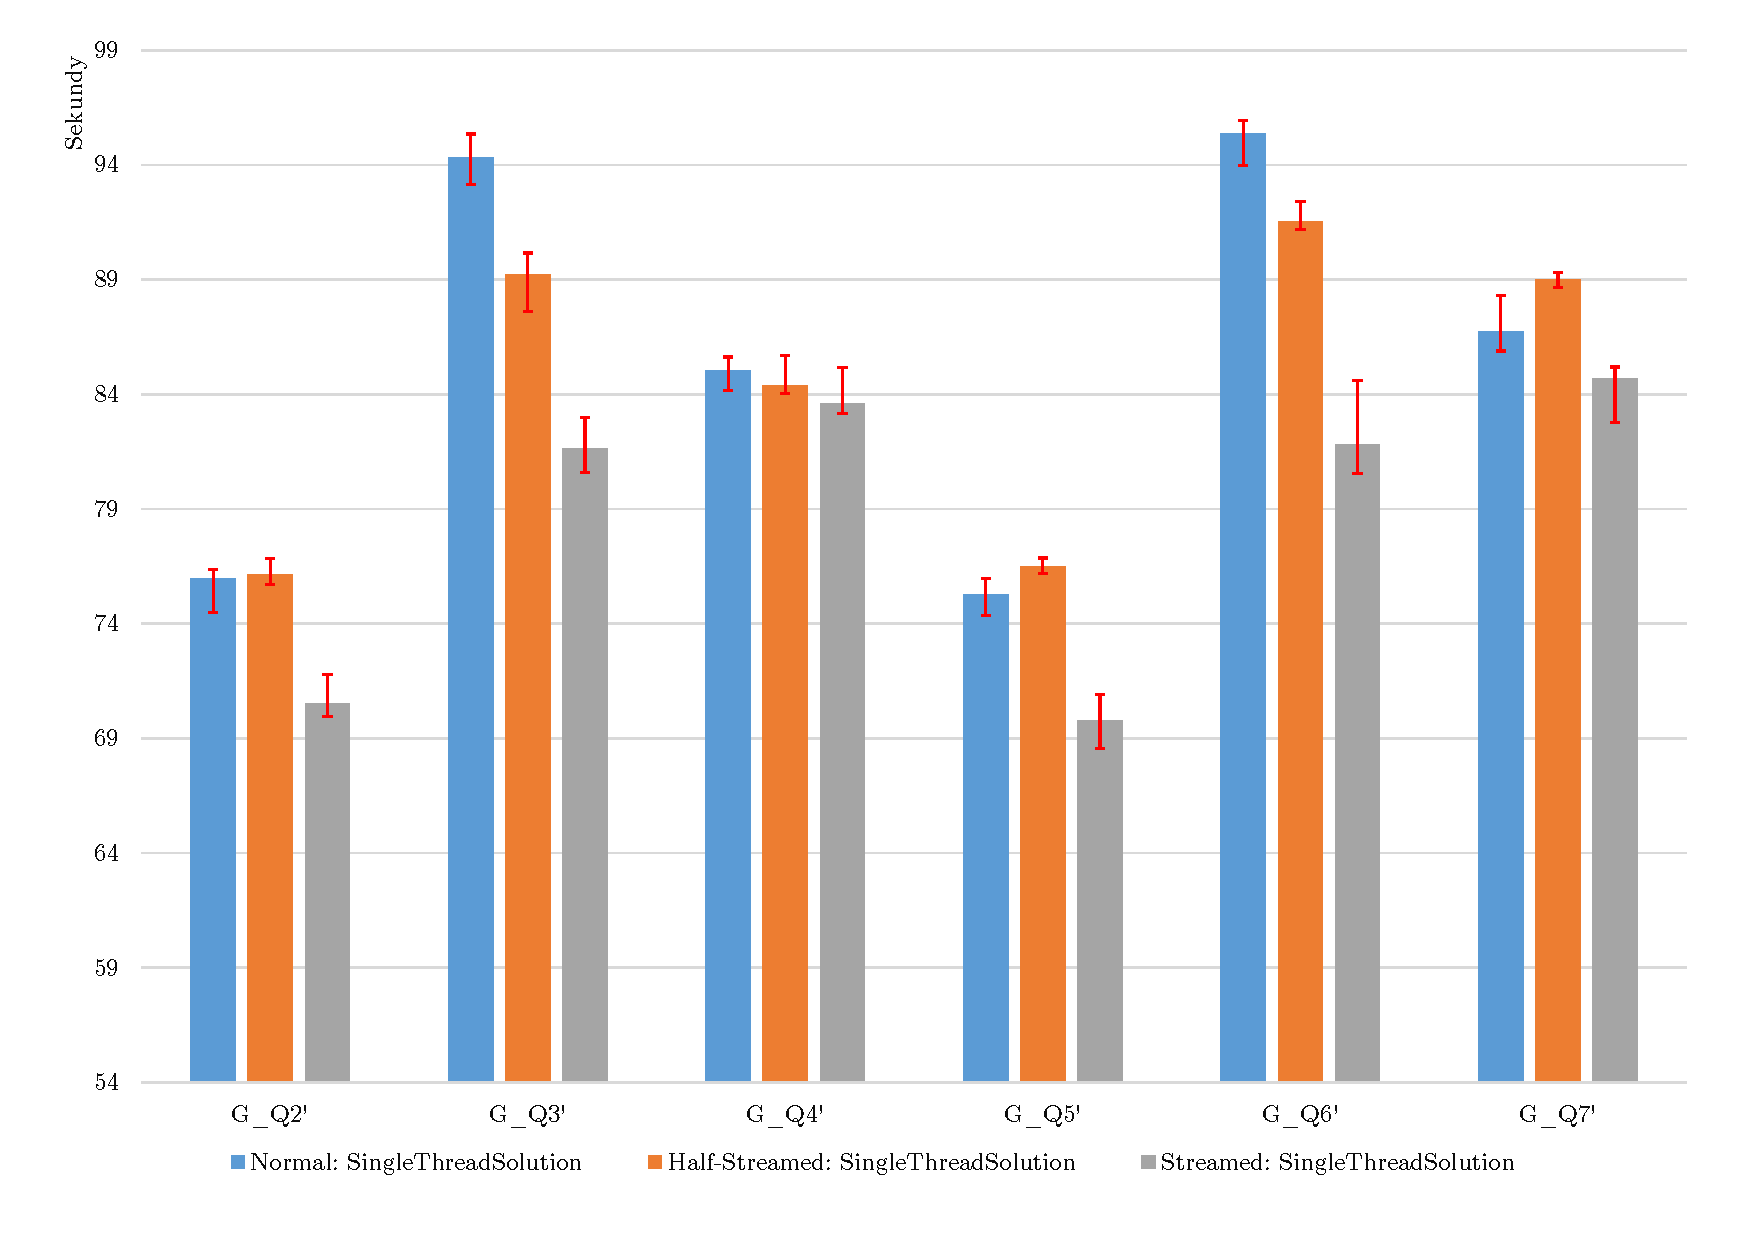
\includegraphics[width=\linewidth]{../img/skitterGroupBySTNoAgg.pdf}\centering
\caption{Doba vykonání dotazů Group by bez agr. funkcí pro graf As-Skitter (sekce \ref{tab.grafBase}). Běh v jednom vláknu.}
\label{figure.skitterGroupBySTNoAgg}
\end{figure}


%%%%%%%%%%%%%%%%%%%%%%%%%%%%

\clearpage

\subsubsection{Obecné shrnutí paralelních řešení} \label{expr.results.groupby.par}

Paralelní řešení používají doposud zmíněná značení.
\textbf{Global} řešení seskupuje výsledky globálně pomocí paralelní mapy (\verb+ConcurrentDictionary+).
\textbf{Two-Step} řešení seskupuje výsledky nejdříve lokálně pomocí mapy a následném sléváním do paralelní mapy.
\textbf{LocalGroupByLocalTwoWayMerge} řešení seskupuje lokálně a následně slévá výsledky vláken po dvojicích. 
Toto slévání si můžeme představit jako binární strom. 
Listy jsou výsledky vláken a vnitřní vrcholy jsou akce slévány.
Výsledky paralelního seskupování jsou zobrazeny na obrázcích před shrnutím výsledků Single group Group by v sekci \ref{expr.results.groupby.sinleGroup}.

\subsubsection{Výsledky paralelního zpracování}

Byli jsme překvapeni, že vylepšená řešení se mnohdy nevyrovnala původním řešením.
\textbf{Streamed} řešení, ačkoliv bylo nejrychlejší v jednovláknovém běhu, tak zde se pouze vyrovnalo \textbf{Normal} řešením a nebo bylo pomalejší.
Danou situaci si vysvětlujeme synchronizací. 
Prvni vrstva synchronizace nastává u přistupu k paralelní mapě a čtení/vložení záznamu.
Po získání \verb+value+ z mapy následuje druhá vrstva, která obsahuje volání thread-safe funkcí pro výpočet agregovaných hodnot pro danou skupinu.
Z obrázků \ref{figure.amazonGQ1Par}, \ref{figure.webberkstanGQ1Par} a \ref{figure.skitterGQ1Par} (\textbf{Streamed} řešení) jsme viděli cenu za synchronizaci na agregačních funkcích při přístupu osmi vláken.

\subsubsection{Test režie paralelní mapy (jedno vlákno)}

Pro představu pouhé režie paralelní mapy jsme otestovali režii zvlášť čtení a vložení \verb+ConcurrentDictionary+ vůči \verb+Dictionary+ pro jedno vlákno.

Následuje příklad kódu použitého při testu (označíme jej \textit{I/Rcode}):
\begin{code}
Random ran = new Random(100100);
Dictionary<int, int> map = new Dictionary<int, int>();
ConcurrentDictionary<int, int> parMap = 
    new ConcurrentDictionary<int, int>();
...
// Insert test. Assuming the maps are empty.
for (int i = 0; i < 1_000_000; i++)
{
    var val = ran.Next();
    // Based on the used map choose (1) or (2).
    (1) if (!map.TryGetValue(val, out int value)) map.Add(val, i);
    (2) var tmp = parMap.GetOrAdd(val, i);
}
...
// Read test. Assuming the maps contain keys from 0 to 1_000_000.
for (int i = 0; i < 100_000_000; i++)
{
    var val = ran.Next(0, 1_000_000);
    // Based on the used map choose (1) or (2).
    (1) if (!map.TryGetValue(val, out int value));
    (2) var tmp = parMap.GetOrAdd(val, val);
}
\end{code}

\subsubsection{Výsledek testu režie paralelní mapy (jedno vlákno)}

\begin{table}[!htb]
\centering
\begin{tabular}{lrrr}
\toprule
\mc{Test} & \mc{\textbf{Dict}} & \mc{\textbf{ConDict}} & \mc{\textbf{ConDict/Dict}} \\
\midrule
\textit{Insert} $10^6$ & 165 & 667 & 4,04  \\
\textit{Insert} $10^7$  & 2476 & 11 272 & 4,55 \\
\textit{Read} $10^8$  & 19 002 & 21 516 & 1,13  \\
\bottomrule
\end{tabular}

\caption{Výsledky testování map v milisekundách.}
\label{tab.mapsInsert}
\end{table}

Měření dle kódu \textit{I/Rcode} výše.
Zkratka \textbf{Dict} označuje \texttt{Dictionary} a zkratka \textbf{ConDict} označuje \texttt{ConcurrentDictionary}.
Běh v jednom vlákně. 
Generování prvků pomocí třídy \texttt{Random} s inicializační hodnotou 100100. 
Měřeno pomocí třídy \texttt{Stopwatch}. 
Výsledek byl zvolen jako průměr pěti měření. 
Test \textit{Insert} $n$ provádí vkládání $n$ náhodně vygenerovaných prvků do prázdné mapy. 
Test \textit{Read} $n$ provádí $n$ čtení z rozsahu 0 až 1 000 000. Poměr je roven podílu času paralelní mapy a mapy.

Tabulka naměřených hodnot testování (\ref{tab.mapsInsert}) ukazuje, že pouhé vkládání náhodně generovaných prvků do paralelní mapy trvá průměrně 4x déle.
Samostatné čtení náhodně generovaných hodnot, které existují v mapě, je průměrně o 13\% pomalejší.

\subsubsection{Test režie paralelní mapy (osm vláken)}

Provedli jsme další test. 
Test bude simulovat vkládání náhodných prvků do paralelní mapy osmi vlákny.
Daná situace je velmi podobná naší situaci v Group by.
Výsledek porovnáme s výsledky režie normální mapy z tabulky \ref{tab.mapsInsert}.

Následuje příklad kódu použitého při testu (označíme jej \textit{ParIcode}):
\begin{code}
ConcurrentDictionary<int, int> parMap = 
    new ConcurrentDictionary<int, int>();
// Insert test. Assuming the maps are empty. (case Insert 10^6)
Parallel.Invoke(
() => Insert(parMap, 0, 125_000, new Random(100100)),
() => Insert(parMap, 125_000, 250_000, new Random(100100)),
...
public static void Insert(ConcurrentDictionary<int, int> dict, 
                          int start, int end, Random ran) {
    for (int i = 0; i < (end - start); i++)
        var v = dict.GetOrAdd(ran.Next(start, end), i); }
\end{code}

%\clearpage

\subsubsection{Výsledek testu režie paralelní mapy (osm vláken)}

\begin{table}[!htb]
\centering
\begin{tabular}{lrrr}
\toprule
\mc{Test} & \mc{\textbf{Dict (1 vlákno)}} & \mc{\textbf{ConDict (8 vláken)}} & \mc{\textbf{ConDict/Dict}} \\
\midrule
\textit{Insert} $10^6$ & 165 & 406 & 2,601  \\
\textit{Insert} $10^7$  & 2476 & 4714 & 1,903 \\
\bottomrule
\end{tabular}

\caption{Výsledky testování map v milisekundách.}
\label{tab.mapsInsertParMap}
\end{table}

Měřeno dle kódu \textit{ParIcode} výše. 
Zkratka \textbf{Dict} označuje \texttt{Dictionary} a zkratka \textbf{ConDict} označuje \texttt{ConcurrentDictionary}. 
\texttt{Dictionary} vykoná práci v jednom vlákně. 
\texttt{ConcurrentDictionary} běží paralelně v osmi vláknech. 
Generování prvků pomocí třídy \texttt{Random} s inicializační hodnotou 100100. 
Měřeno pomocí třídy \texttt{Stopwatch}. 
Výsledek zvolen jako průměr pěti měření. 
Test \textit{Insert} $n$ provádí vkládání $n$ náhodně vygenerovaných prvků do prázdné mapy. 
Poměr je roven podílu času paralelní mapy a mapy. Každé vlákno vkládá stejný počet náhodně generovaných prvků z určitého rozsahu.

Z tabulky porovnání vkládání \ref{tab.mapsInsertParMap} vidíme, že samotná paralelizace je pro náš počet vkládání prvků pomalejší. 
Tedy obecné zpomalení je zřetelné u řešení používající paralelní mapu.

\subsubsection{Paralelní Streamed řešení vs paralelní Normal: Global řešení}

\textbf{Streamed} řešení vůči jeho protějšku \textbf{Normal: Global} je místy pomalejší. 
Děje se tak ve dvou grafech.
První je graf As-Skitter u dotazů  G\_3/G\_3$'$ a  G\_6/G\_6$'$.
Druhý graf je Amazon0601 na dotazech G\_4/G\_4$'$ a  G\_5/G\_5$'$.
Myslíme si, že se jedná o specifické situace pro dané grafy a nedokážeme je plně zodpovědět, jelikož navzájem a pro graf WebBerkStan nenastávají.
Obecně pro dotazy G\_6/G\_6$'$ až G\_8/G\_8$'$ vidíme mírné zrychlení \textbf{Streamed} řešení, protože šetří drahou réžii za vytváření nových skupin.
Pro \textbf{Normal: Global} nastává zpomalení, jelikož se při vkládání do mapy častěji vyvolá drahé porovnání klíčů pomocí vlastností skrze tabulku výsledků. 

\subsubsection{Aplikace poznatků jednovláknového zpracování při paralelním zpracování}

Můžeme zde aplikovat poznatky z výsledků jednovláknových řešení pro \textbf{Normal: Two-Step} proti \textbf{Half-Streamed: Two-Step}.
\textbf{Half-Streamed} řešení je zde opět pomalejší než \textbf{Normal} řešení nebo jsou vyrovnané.
Dále zde opět vidíme zpomalení implementace List vůči Bucket, které jsme viděli u jednovláknových řešení.
Situace při které je List rychlejší nastávala pro dotazy G\_Q4 a G\_Q5 na grafu Amazon0601 a WebBerkStan.
Nyní nastává pouze pro graf Amazon0601 s řešením \textbf{Normal: LocalGroupByLocalTwoWayMerge}.
Two-step (List) řešení při slévání překopírovává větší množství dat, proto u něj daný jev už nenastává. 

\subsubsection{Nejrychlejší paralelní řešení}

Všem řešením dominuje\textbf{Normal: LocalGroupByLocalTwoWayMerge},\\* které provádí vše lokálně a ujišťuje nás v předpokladu, že hlavní důvod zpomalení je synchronizace.
Například dané řešení vůči \textbf{Normal: Two-Step}. 
Je zde vidět režie za použití paralelní mapy vůči lokálnímu slévání po dvojicích, jelikož samotný první krok je totožný pro obě řešení.
Zpomalení \textbf{Normal: Two-Step} je ještě znatelnější pro dotazy G\_Q4/G\_Q4$'$ a G\_Q5/G\_Q5$'$, kdy se vkládá množství skupin do paralelní mapy.

\bigskip
Z výsledků usuzujeme, že vylepšená řešení pro náš případ paralelizace neposkytují z hlediska rychlosti vykonání znatelné výhody oproti stávajícím řešením.

\begin{figure}[!htp]
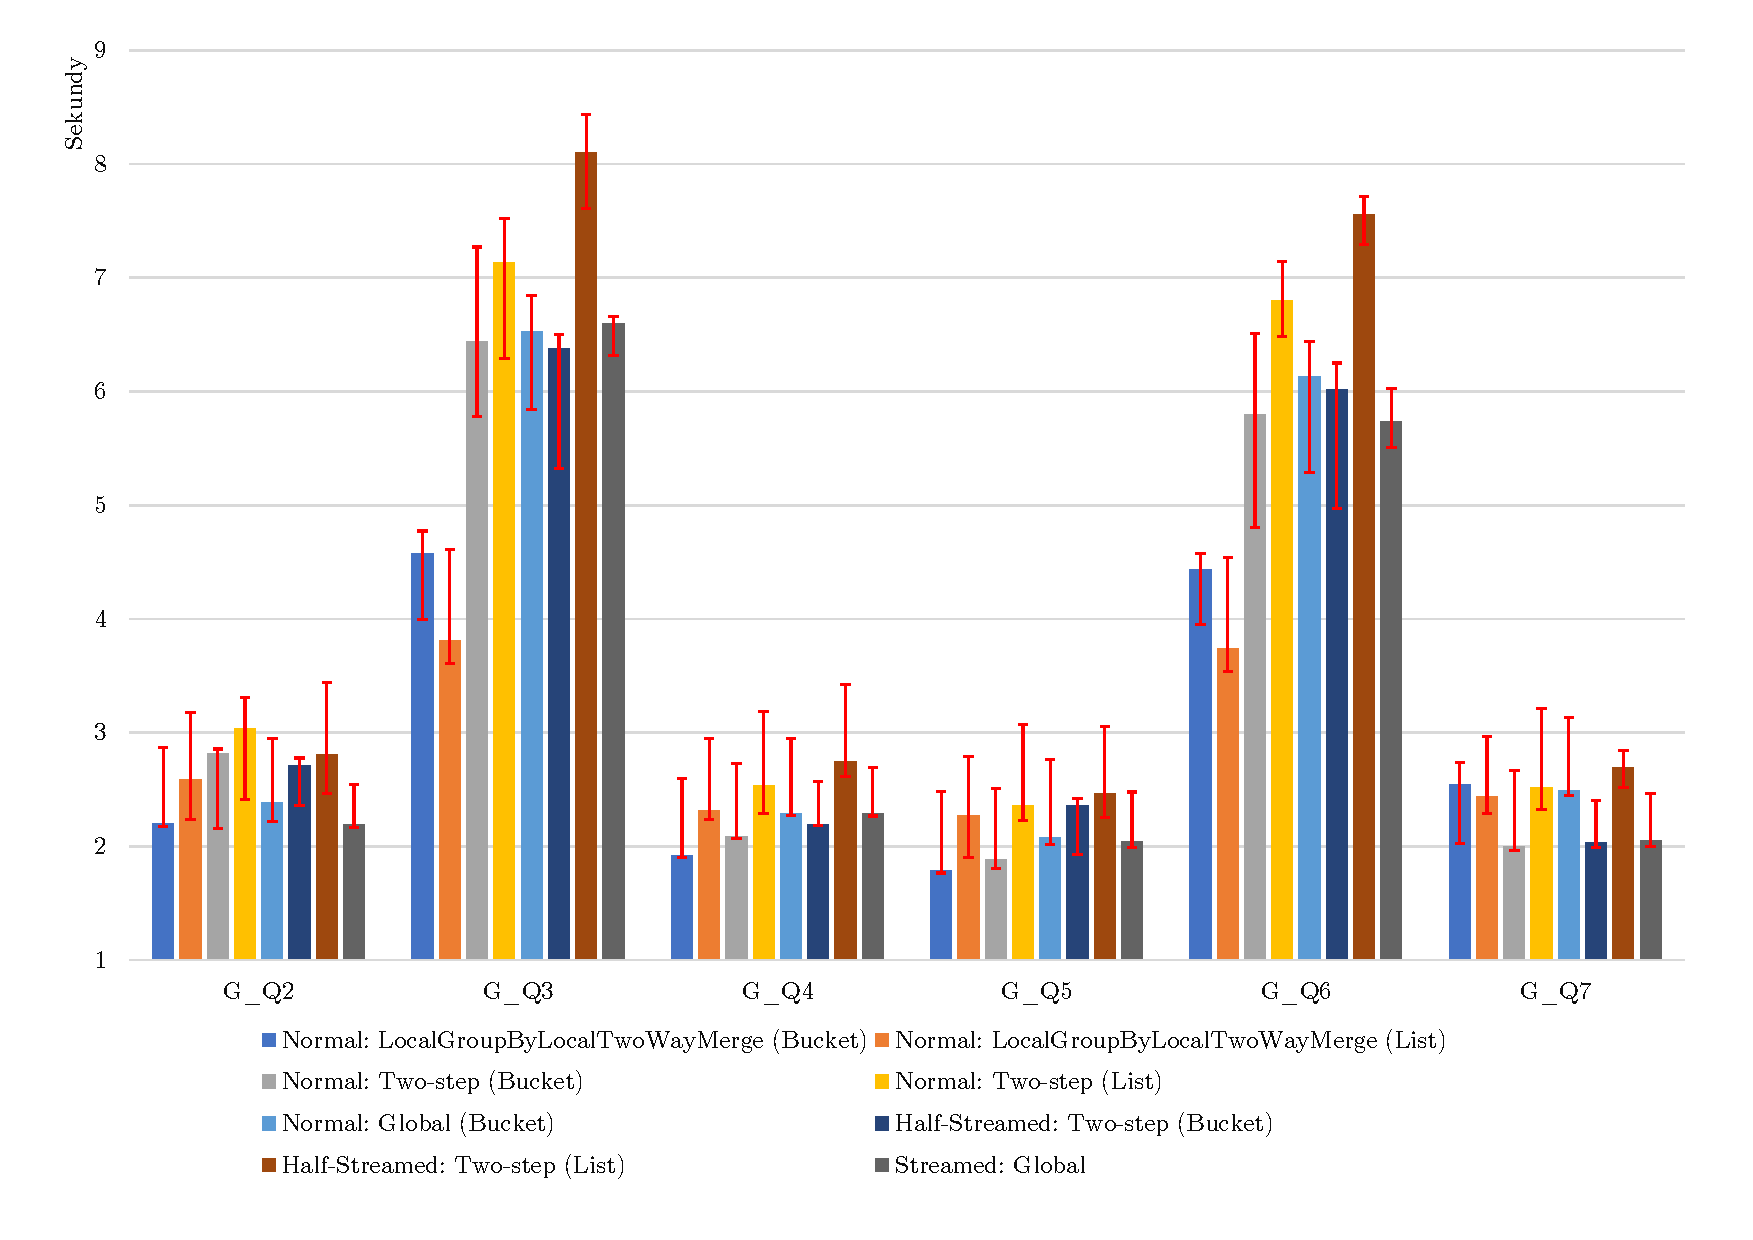
\includegraphics[width=\linewidth]{../img/amazonGroupByPar.pdf}\centering
\caption{Doba vykonání dotazů Group by pro graf Amazon0601 (sekce \ref{tab.grafBase}). Běh osmi vláken.}
\label{figure.amazonGroupByPar}
\end{figure}
\begin{figure}[!htp]
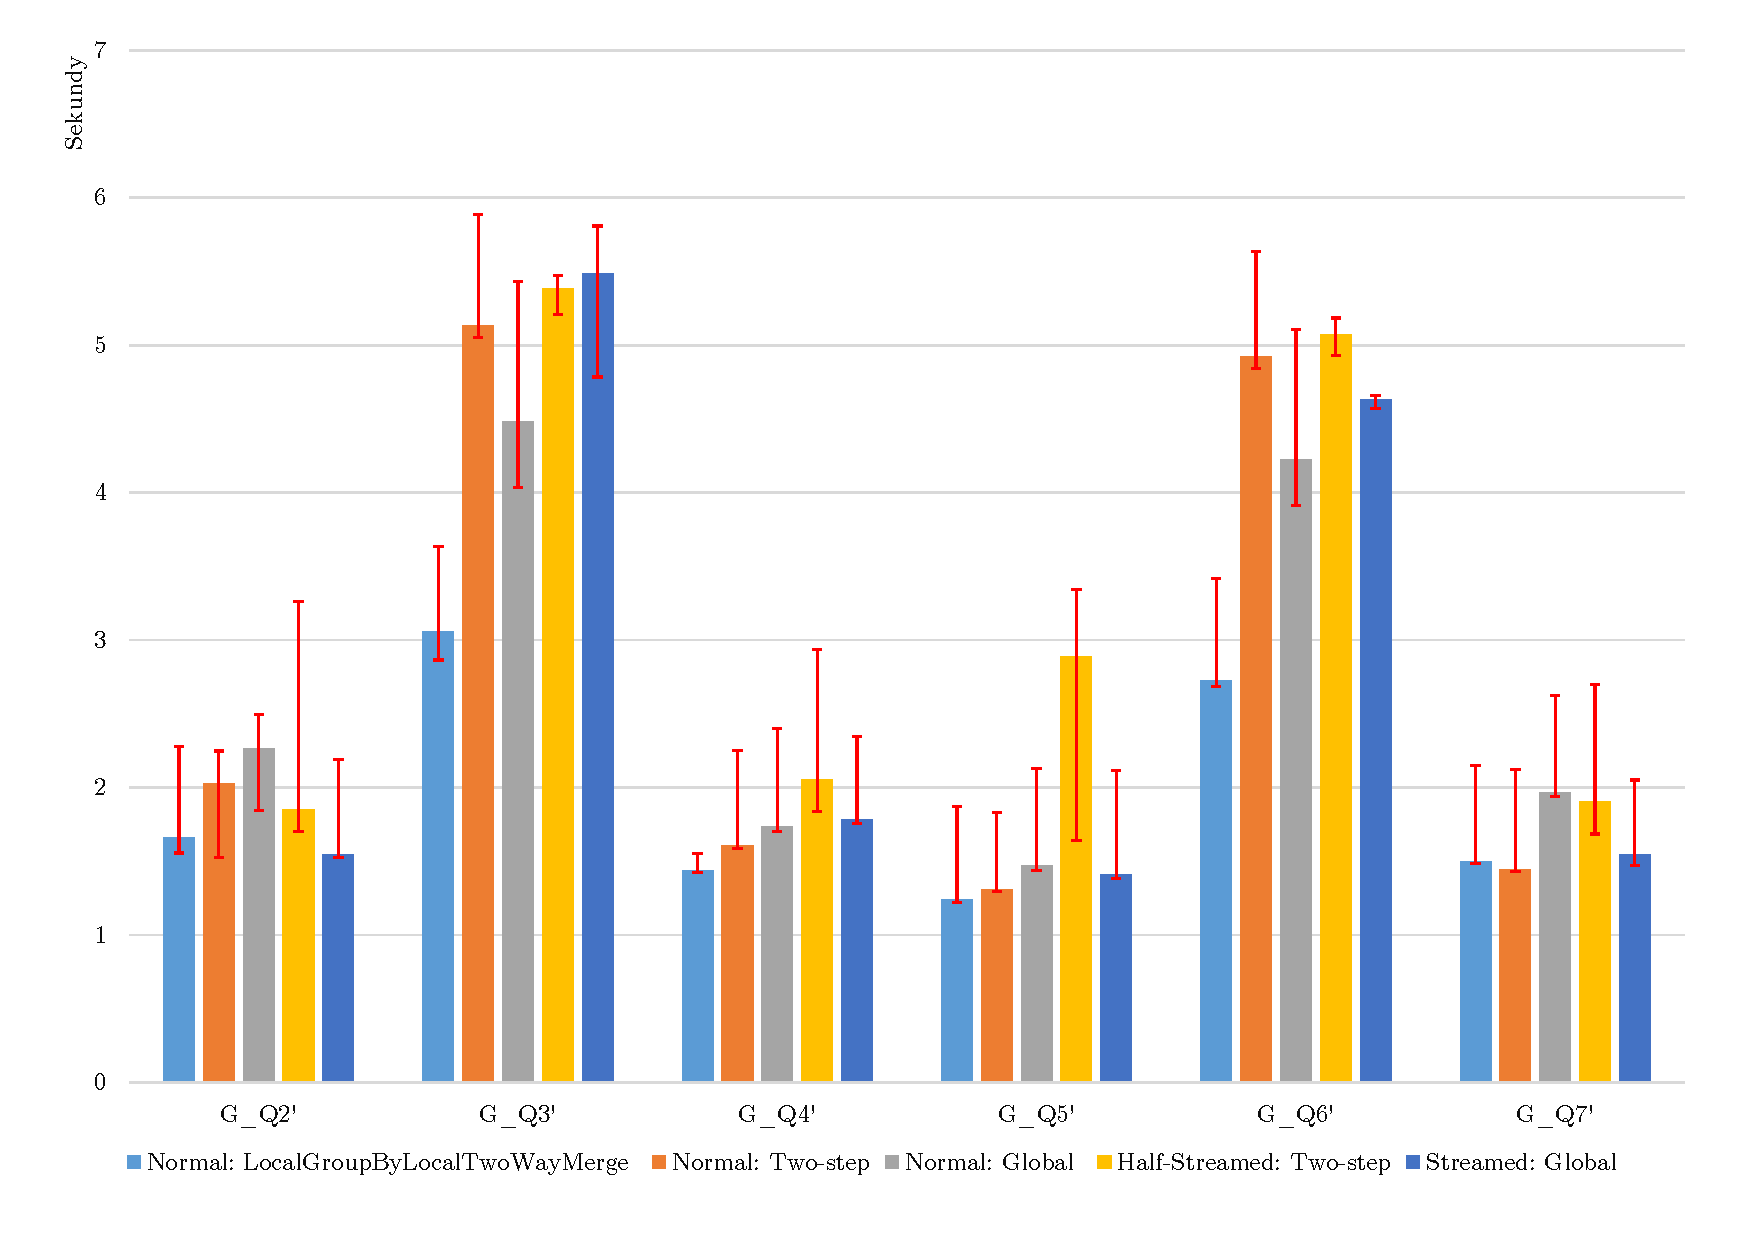
\includegraphics[width=\linewidth]{../img/amazonGroupByParNoAgg.pdf}\centering
\caption{Doba vykonání dotazů Group by bez agr. funkcí pro graf Amazon0601 (sekce \ref{tab.grafBase}). Běh osmi vláken.}
\label{figure.amazonGroupByParNoAgg}
\end{figure}

\begin{figure}[!htp]
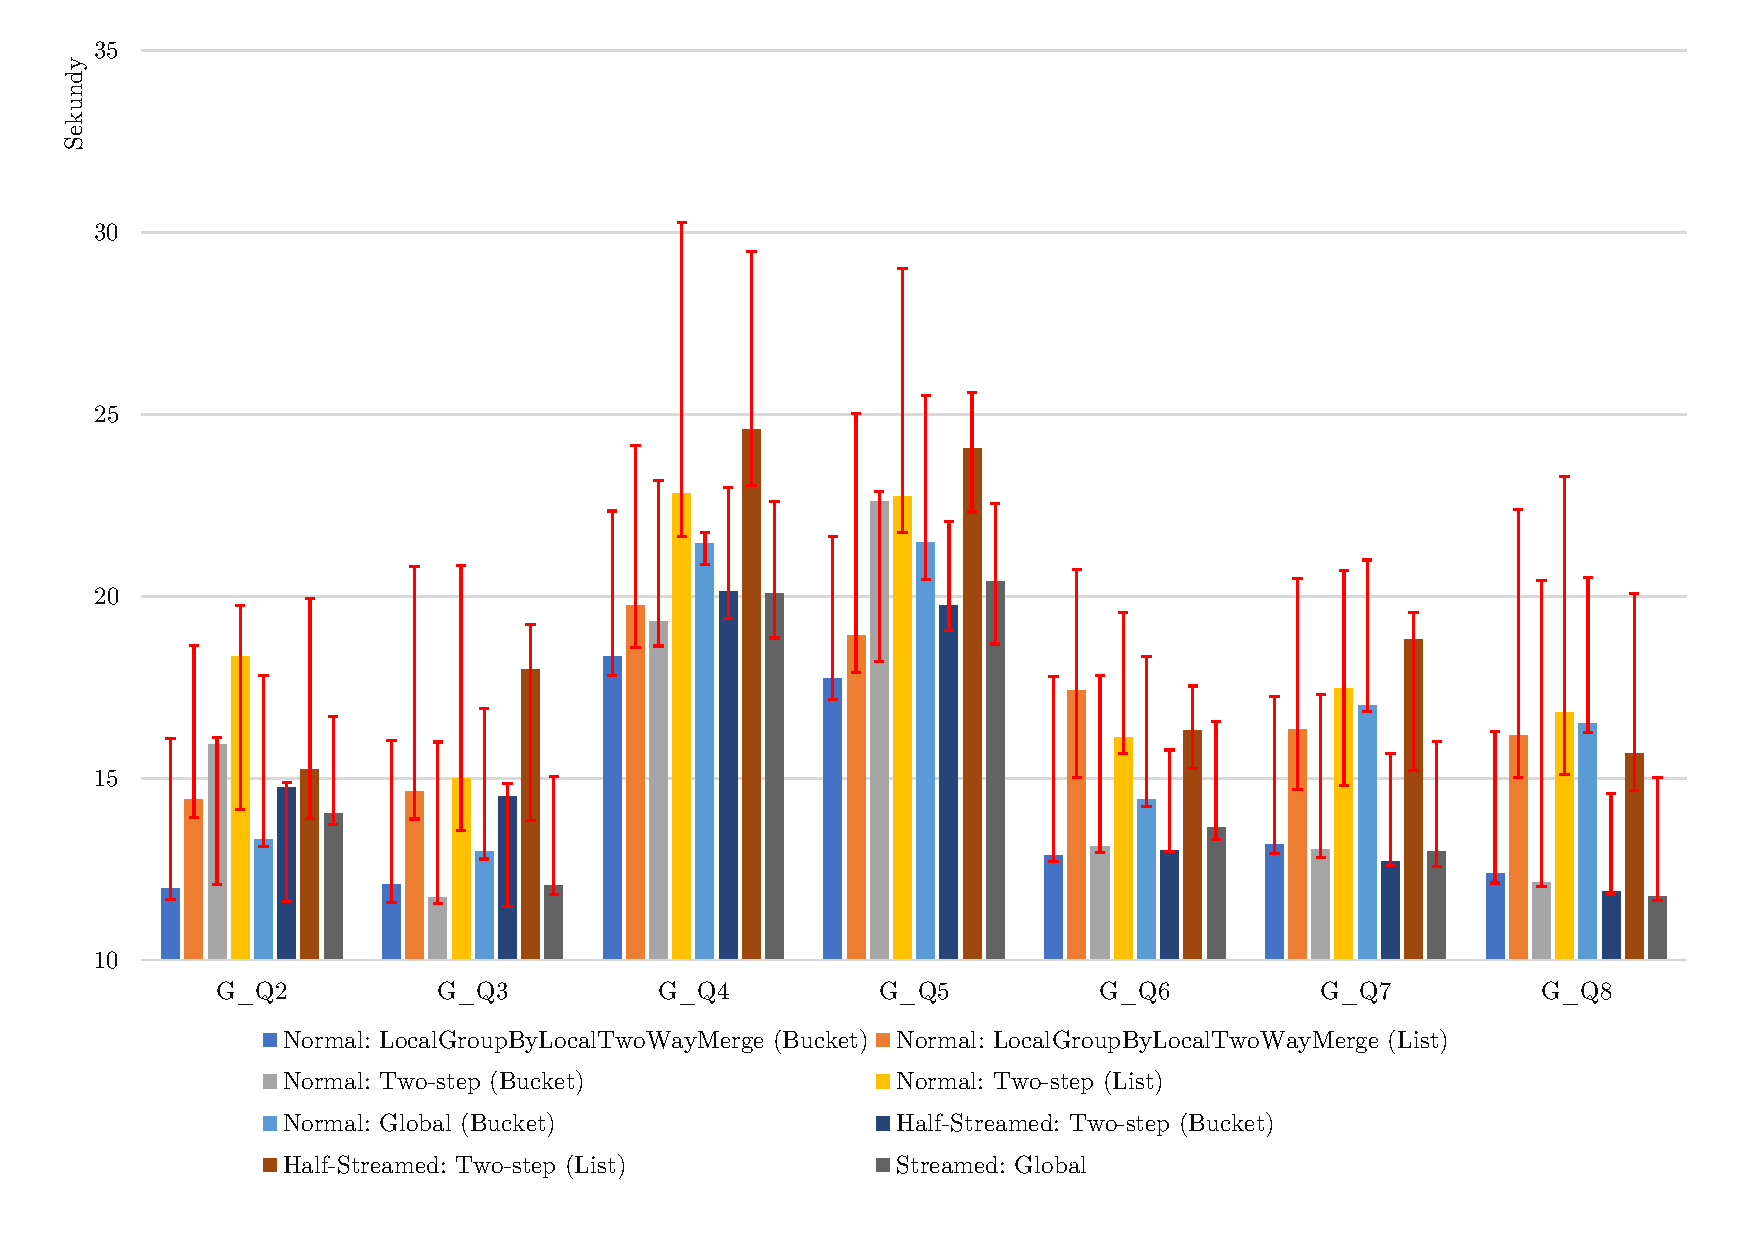
\includegraphics[width=\linewidth]{../img/webberkstanGroupByPar.pdf}\centering
\caption{Doba vykonání dotazů Group by pro graf WebBerkStan (sekce \ref{tab.grafBase}). Běh osmi vláken.}
\label{figure.webberkstanGroupByPar}
\end{figure}
\begin{figure}[!htp]
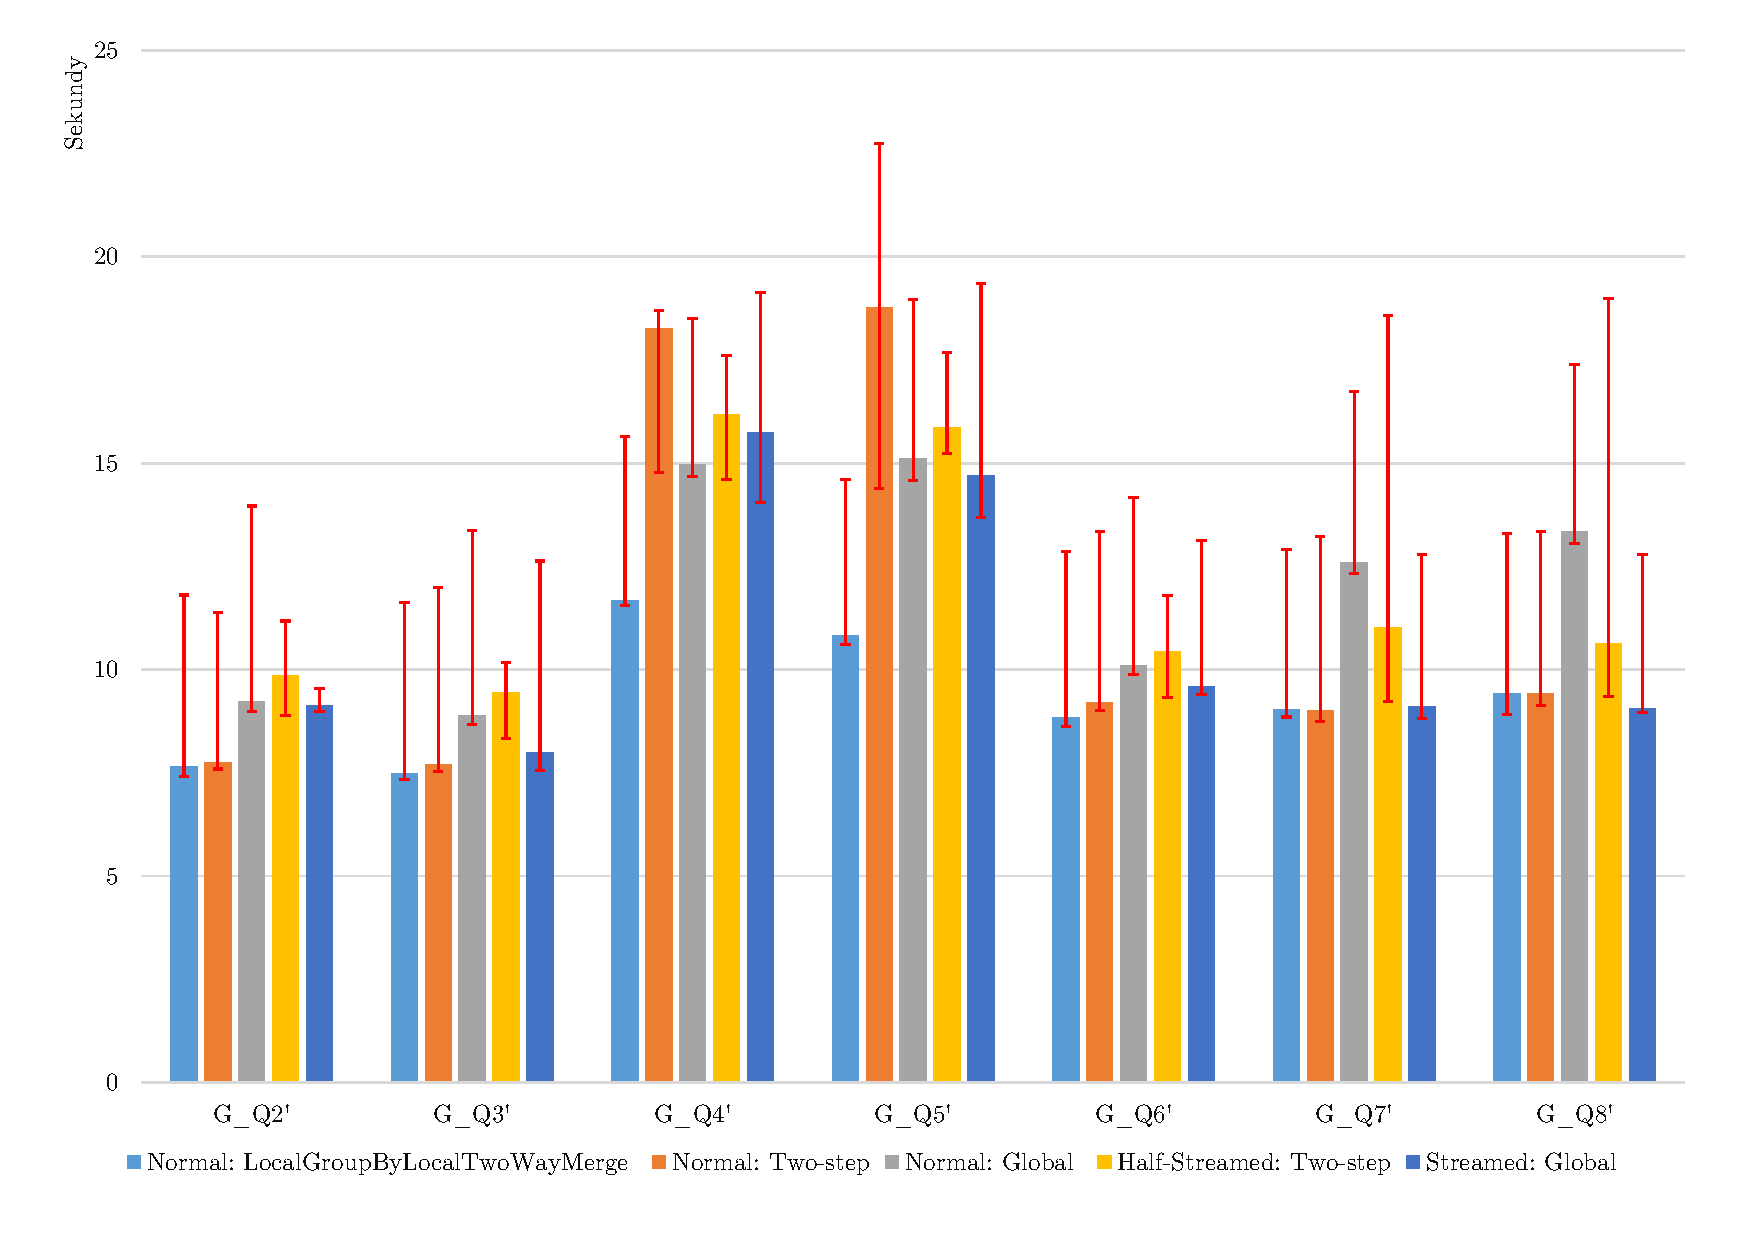
\includegraphics[width=\linewidth]{../img/webberkstanGroupByParNoAgg.pdf}\centering
\caption{Doba vykonání dotazů Group by bez agr. funkcí pro graf WebBerkStan (sekce \ref{tab.grafBase}). Běh osmi vláken.}
\label{figure.webberkstanGroupByParNoAgg}
\end{figure}

\begin{figure}[!htp]
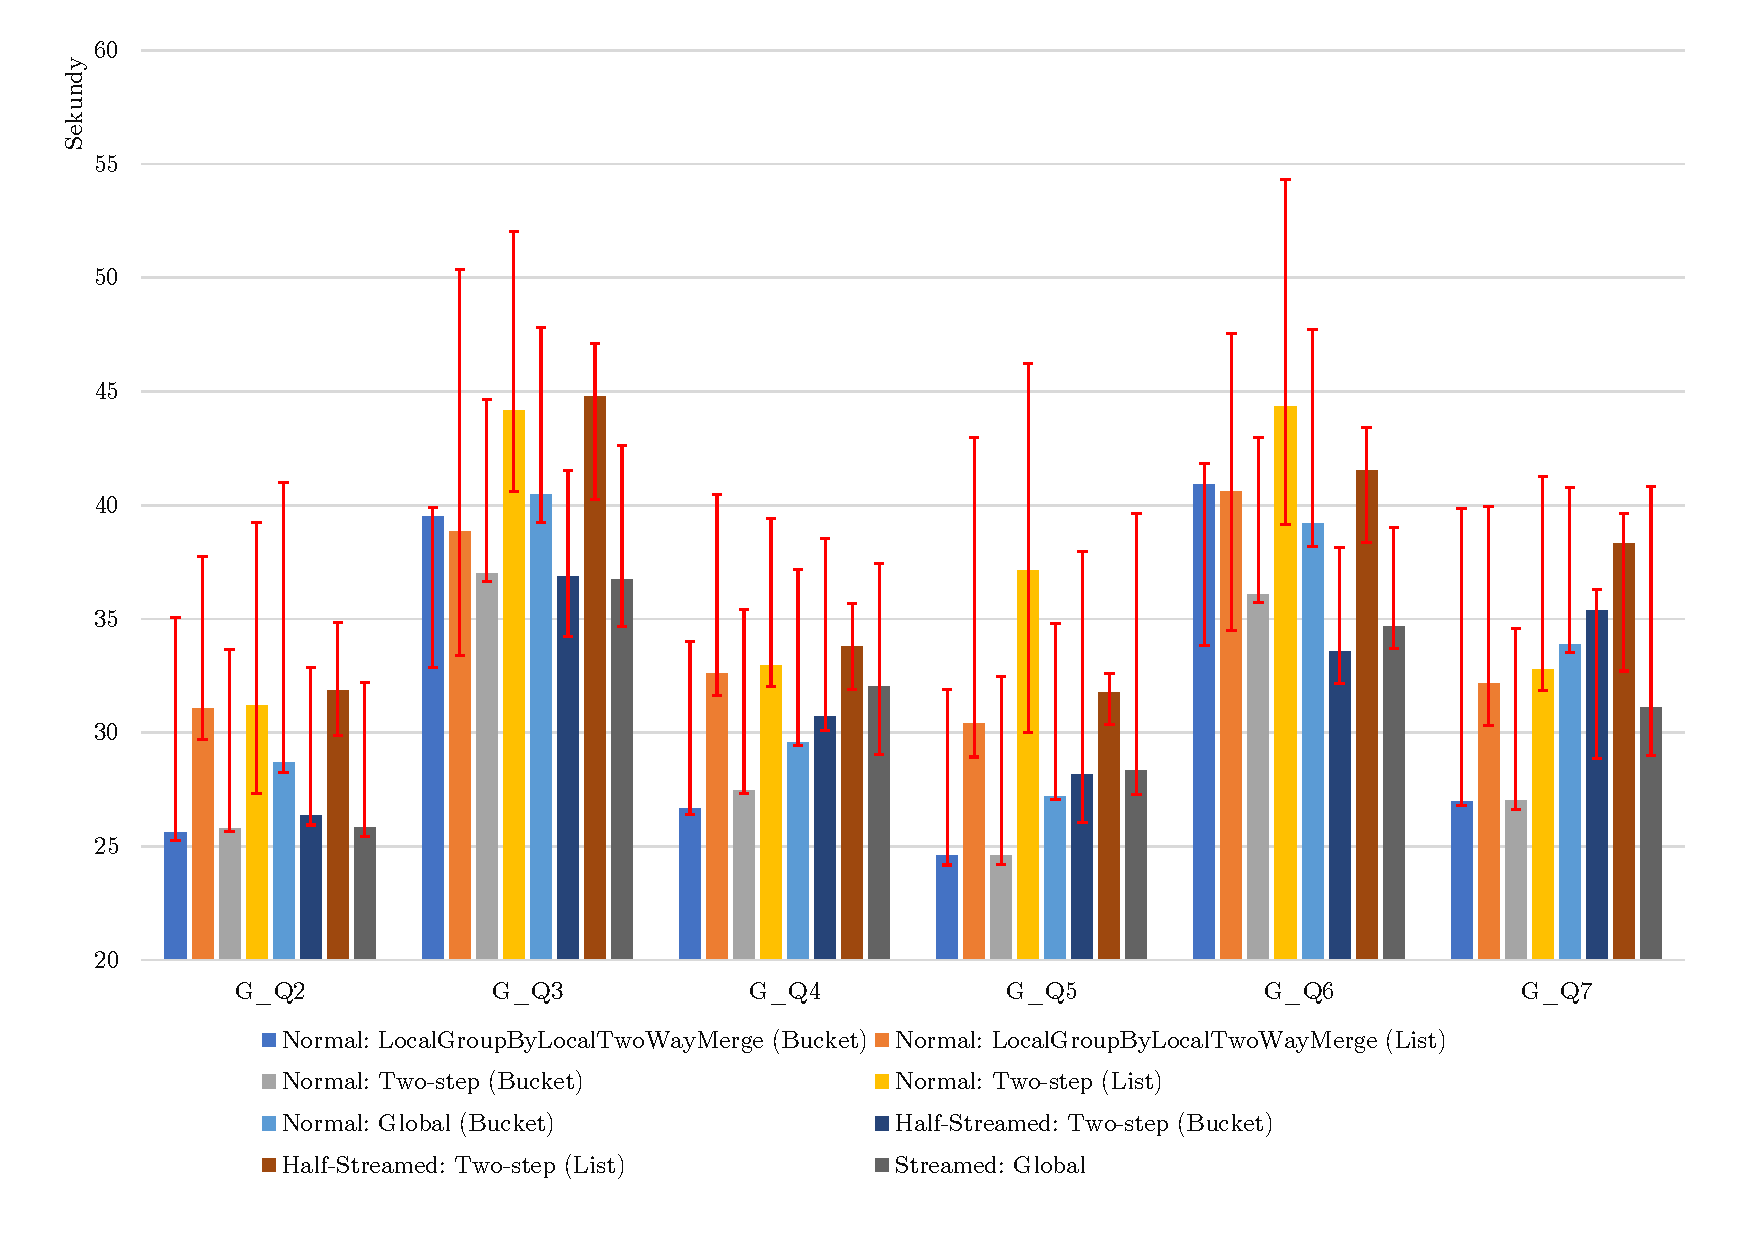
\includegraphics[width=\linewidth]{../img/skitterGroupByPar.pdf}\centering
\caption{Doba vykonání dotazů Group by pro graf As-Skitter (sekce \ref{tab.grafBase}). Běh osmi vláken.}
\label{figure.skitterGroupByPar}
\end{figure}
\begin{figure}[!htp]
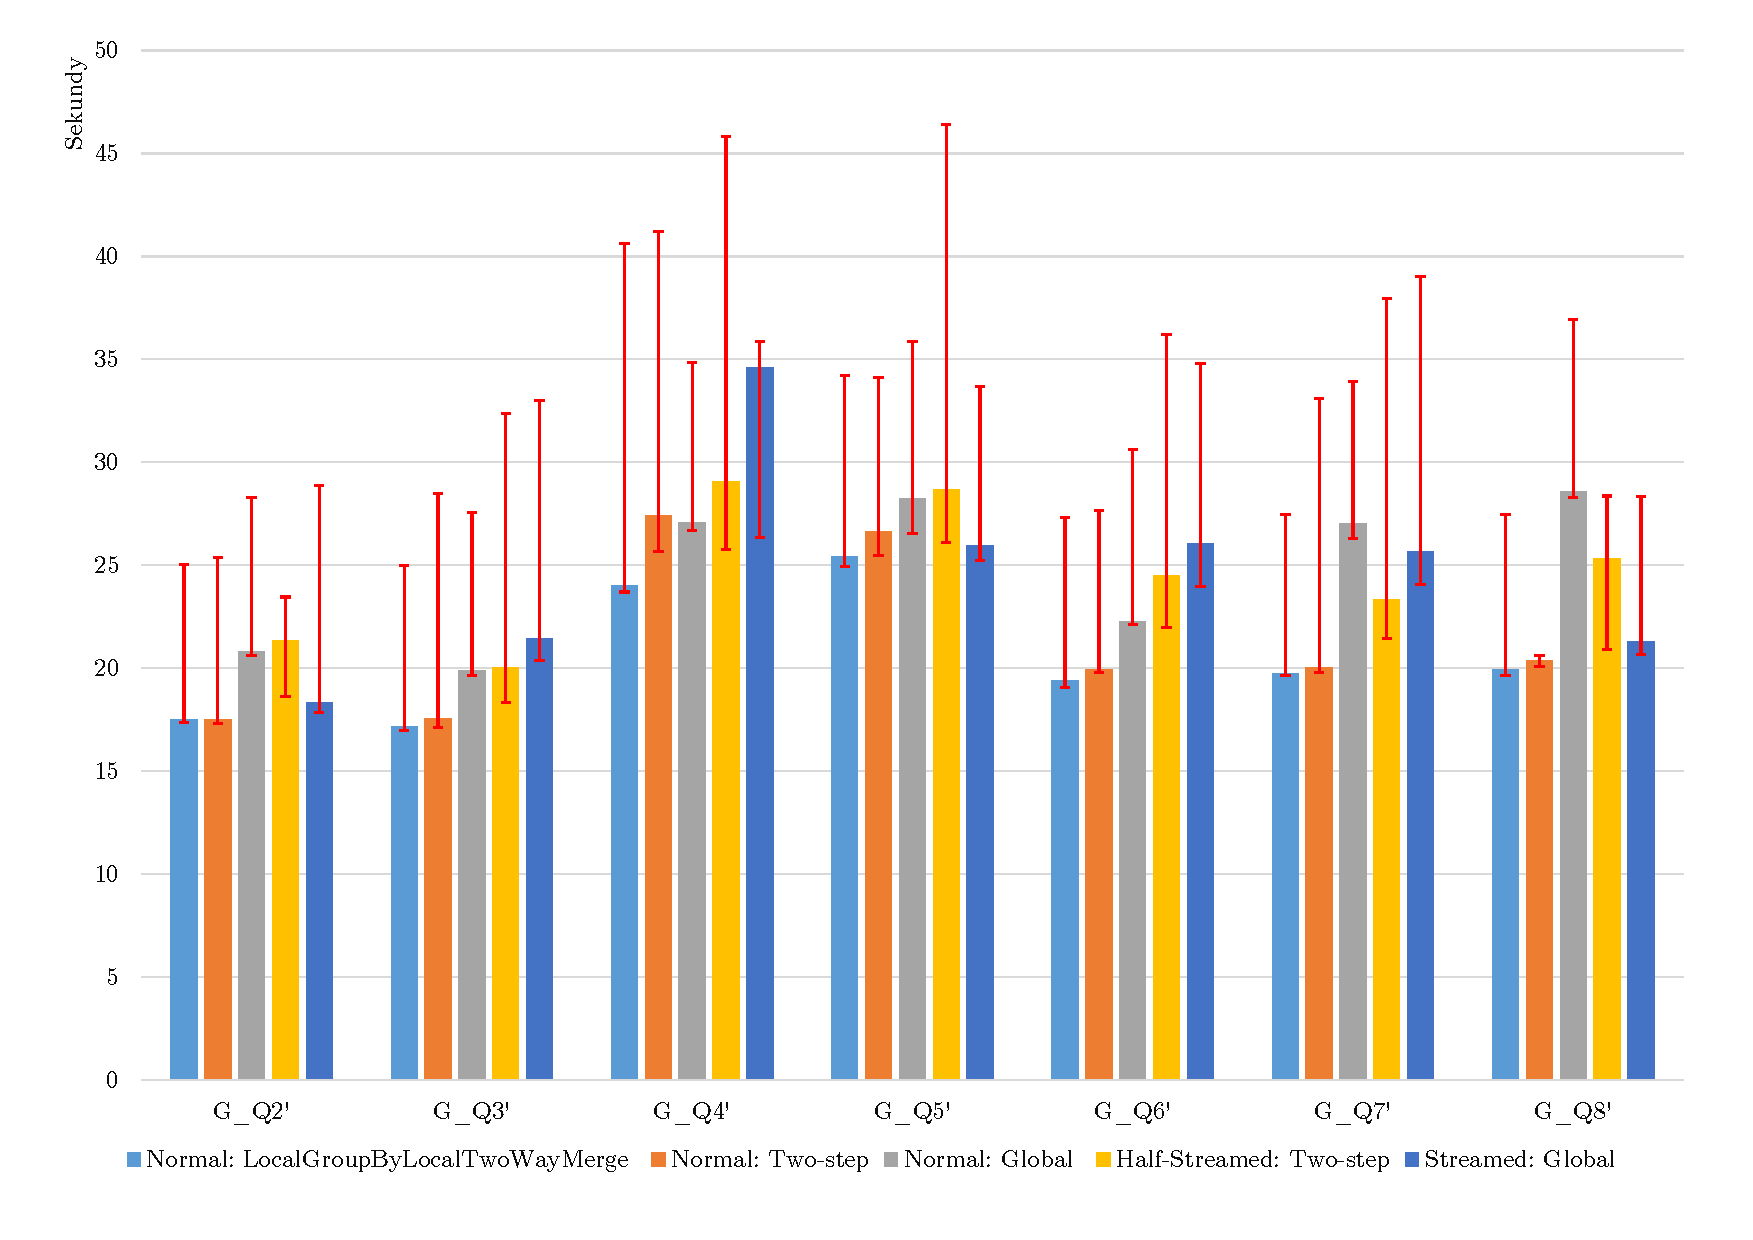
\includegraphics[width=\linewidth]{../img/skitterGroupByParNoAgg.pdf}\centering
\caption{Doba vykonání dotazů Group by bez agr. funkcí pro graf As-Skitter (sekce \ref{tab.grafBase}). Běh osmi vláken.}
\label{figure.skitterGroupByParNoAgg}
\end{figure}
\bigskip

\subsubsection{Obecné shrnutí Single group Group by řešení} \label{expr.results.groupby.sinleGroup}

Analýzu výsledků dotazu G\_Q1 uvádíme samostatně, protože testuje pouze agregační funkce a nikoliv seskupování.
Daný mód Group by předpokládá, že všechny výsledky patří do stejné skupiny a tedy nedochází k seskupování ale pouze k výpočtu agregačních funkcí.
Jednovláknové \textbf{Normal} řešeni iteruje skrze všechny výsledky po dokončení vyhledávání a vypočte agregační funkce.
Jednovláknové \textbf{Half-Streamed} a \textbf{Streamed} řešení jsou totožná.
V průběhu prohledávání aktualizují hodnotu agregační funkce a výsledek zahodí. 
Paralelní \textbf{Normal} řešení všem vláknům přidělí stejný počet výsledů prohledávání a každé lokálně spočte hodnoty agregačních funkcí.
Po ukončení práce všech vláken jedno vybrané vlákno sloučí výsledky všech ostatních vláken. 
Rešení \textbf{Half-Streamed} provádí stejnou práci jako v jednovláknovém zpracování.
Po dokončení prohledávání dojde ke sloučení všech lokálních výsledků.
\textbf{Streamed} řešení pracuje se sdíleným úložištěm výsledků a použivá thread-safe funkce k aktualizaci výsledků.
Obě řešení výsledky neukládají.

\begin{figure}[!htp]
    \centering
    \begin{minipage}{0.45\textwidth}
        \centering
        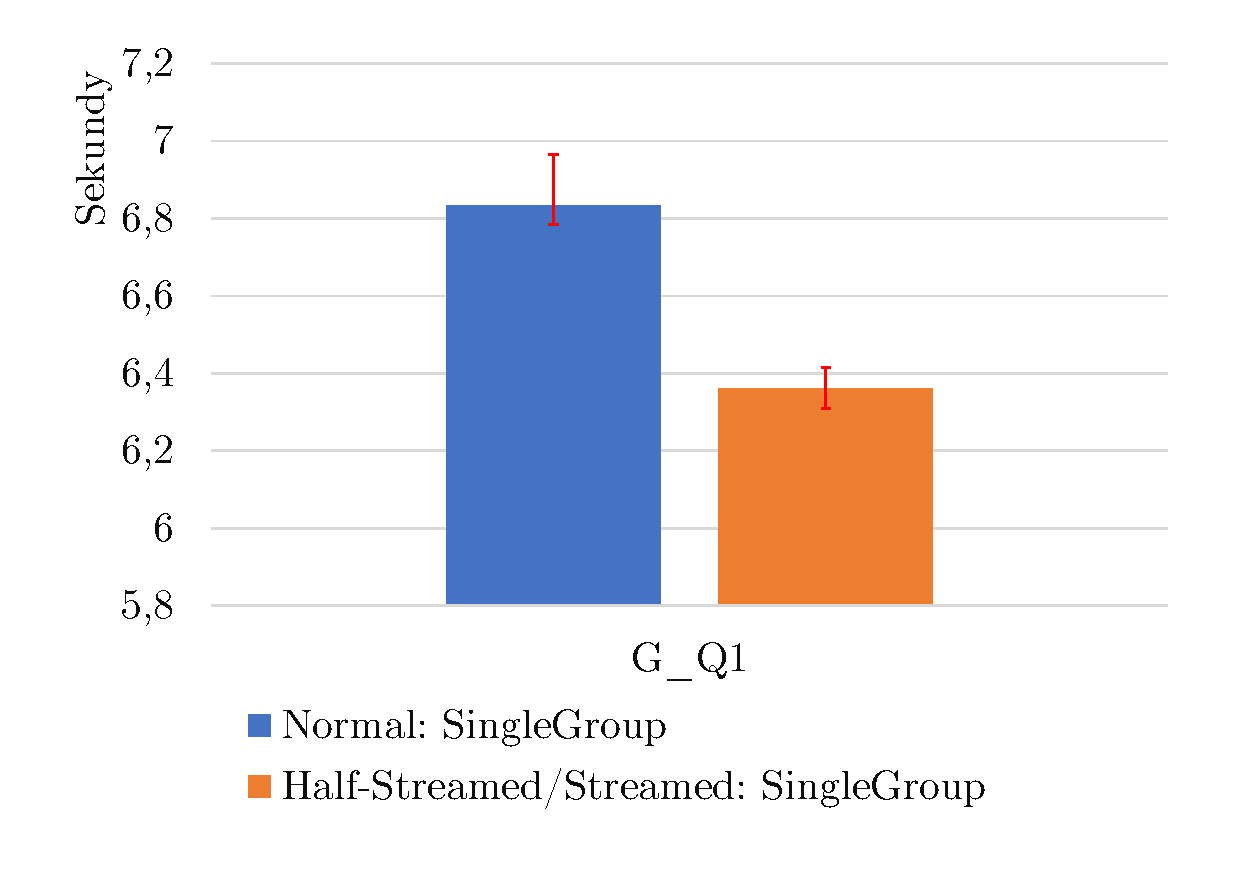
\includegraphics[width=0.9\textwidth]{../img/amazonGroupByQ1ST.pdf} % first figure itself
        \caption{Doba vykonání dotazu G\_Q1 pro graf Amazon0601 (sekce \ref{tab.grafBase}). Běh v jednom vláknu.}
        \label{figure.amazonGQ1ST}
    \end{minipage}\hfill
    \begin{minipage}{0.45\textwidth}
        \centering
        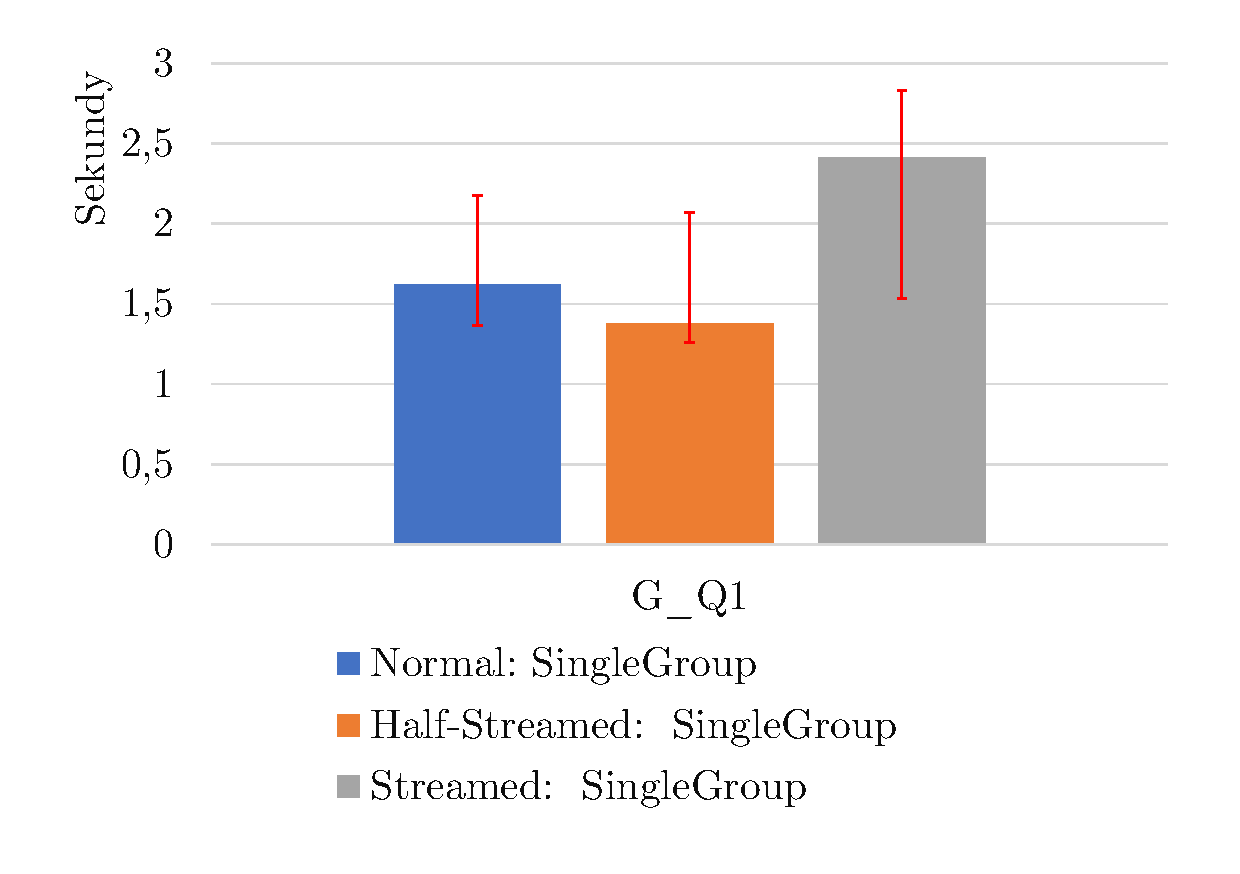
\includegraphics[width=0.9\textwidth]{../img/amazonGroupByQ1Par.pdf} % second figure itself
        \caption{Doba vykonání dotazu G\_Q1 pro graf Amazon0601 (sekce \ref{tab.grafBase}). Běh osmi vláken.}
        \label{figure.amazonGQ1Par}
    \end{minipage}
\end{figure}

\begin{figure}[!htp]
    \centering
    \begin{minipage}{0.45\textwidth}
        \centering
        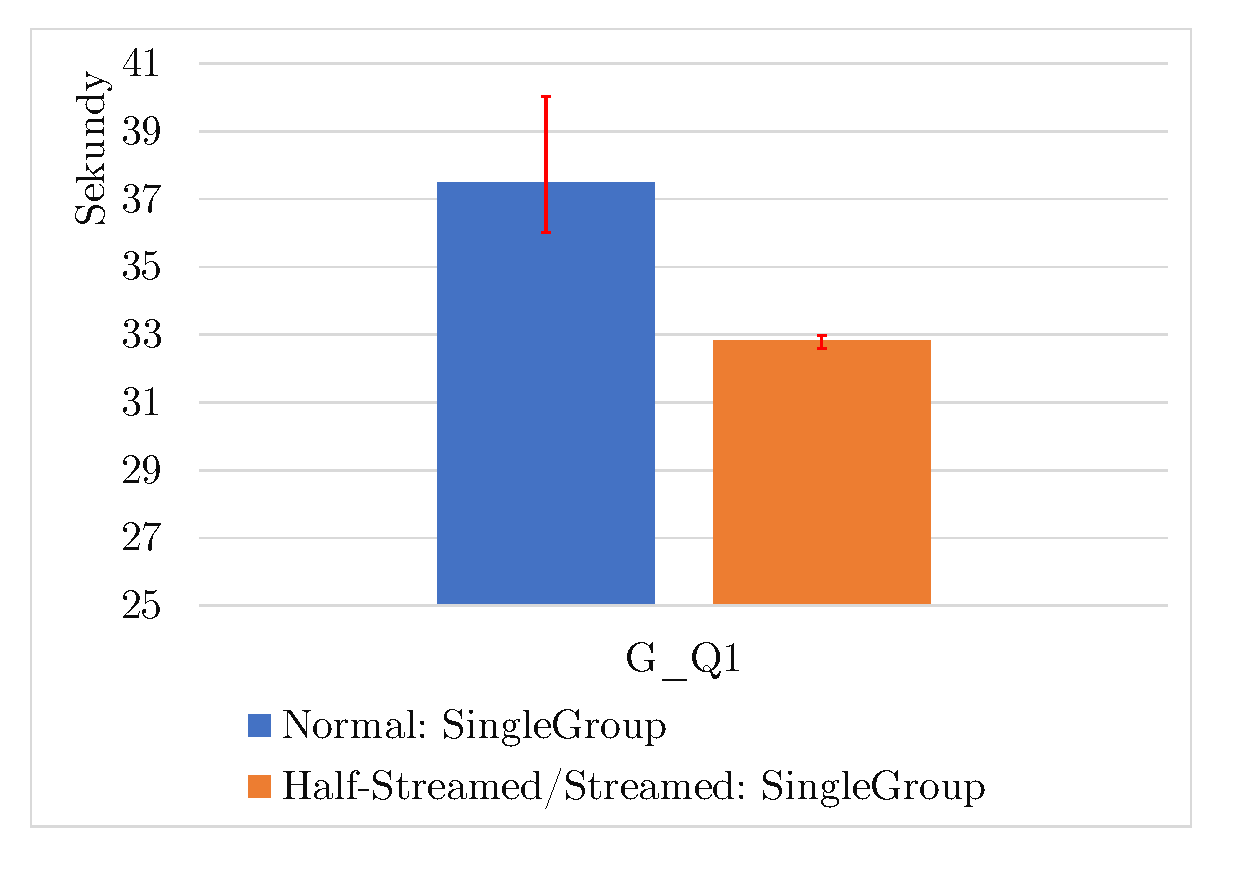
\includegraphics[width=0.9\textwidth]{../img/webberkstanGroupByQ1ST.pdf} % first figure itself
        \caption{Doba vykonání dotazu G\_Q1 pro graf WebBerkStan (sekce \ref{tab.grafBase}). Běh v jednom vláknu.}
        \label{figure.webberkstanGQ1ST}
    \end{minipage}\hfill
    \begin{minipage}{0.45\textwidth}
        \centering
        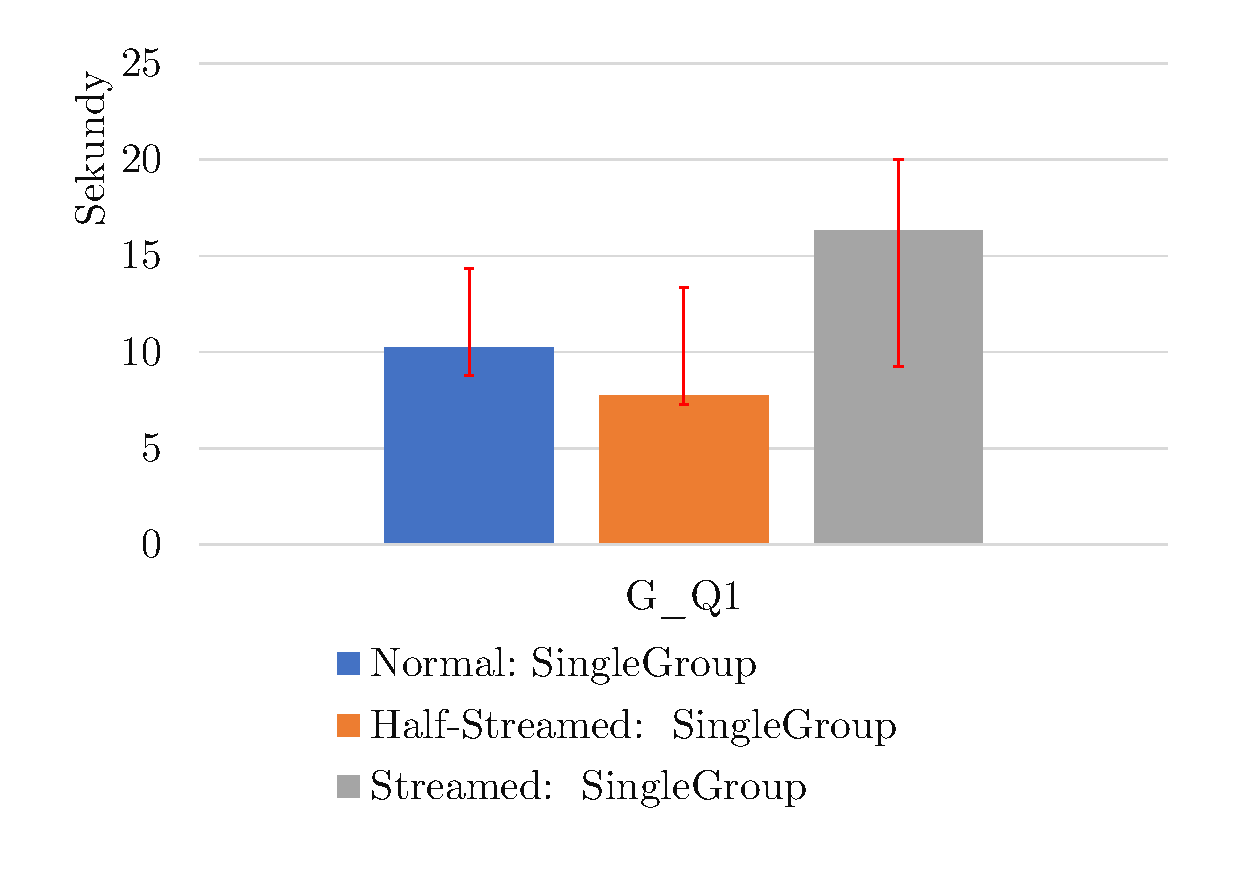
\includegraphics[width=0.9\textwidth]{../img/webberkstanGroupByQ1Par.pdf} % second figure itself
        \caption{Doba vykonání dotazu G\_Q1 pro graf WebBerkStan (sekce \ref{tab.grafBase}). Běh osmi vláken.}
        \label{figure.webberkstanGQ1Par}
    \end{minipage}
\end{figure}
\clearpage
\begin{figure}[!htp]
    \centering
    \begin{minipage}{0.45\textwidth}
        \centering
        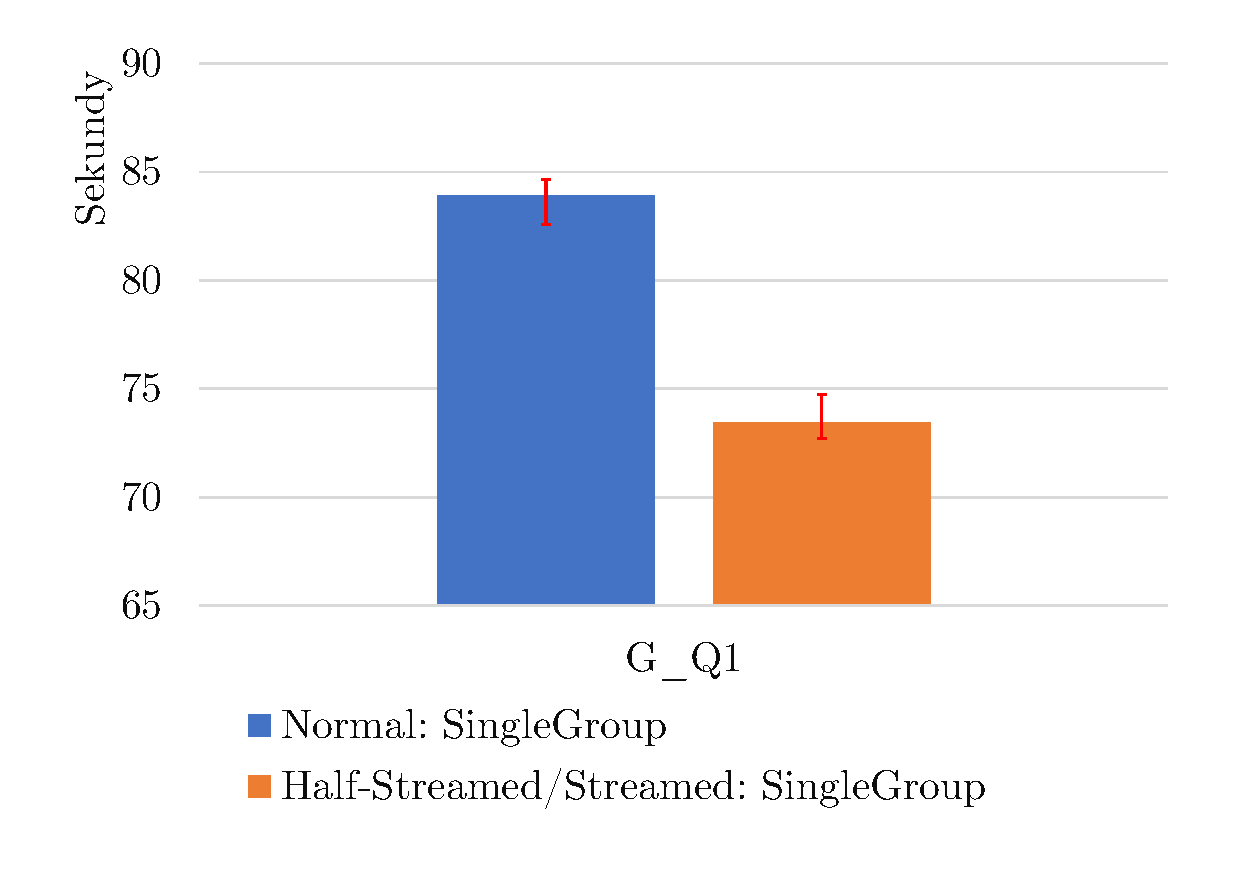
\includegraphics[width=0.9\textwidth]{../img/skitterGroupByQ1ST.pdf} % first figure itself
        \caption{Doba vykonání dotazu G\_Q1 pro graf As-Skitter (sekce \ref{tab.grafBase}). Běh v jednom vláknu.}
        \label{figure.skitterGQ1ST}
    \end{minipage}\hfill
    \begin{minipage}{0.45\textwidth}
        \centering
        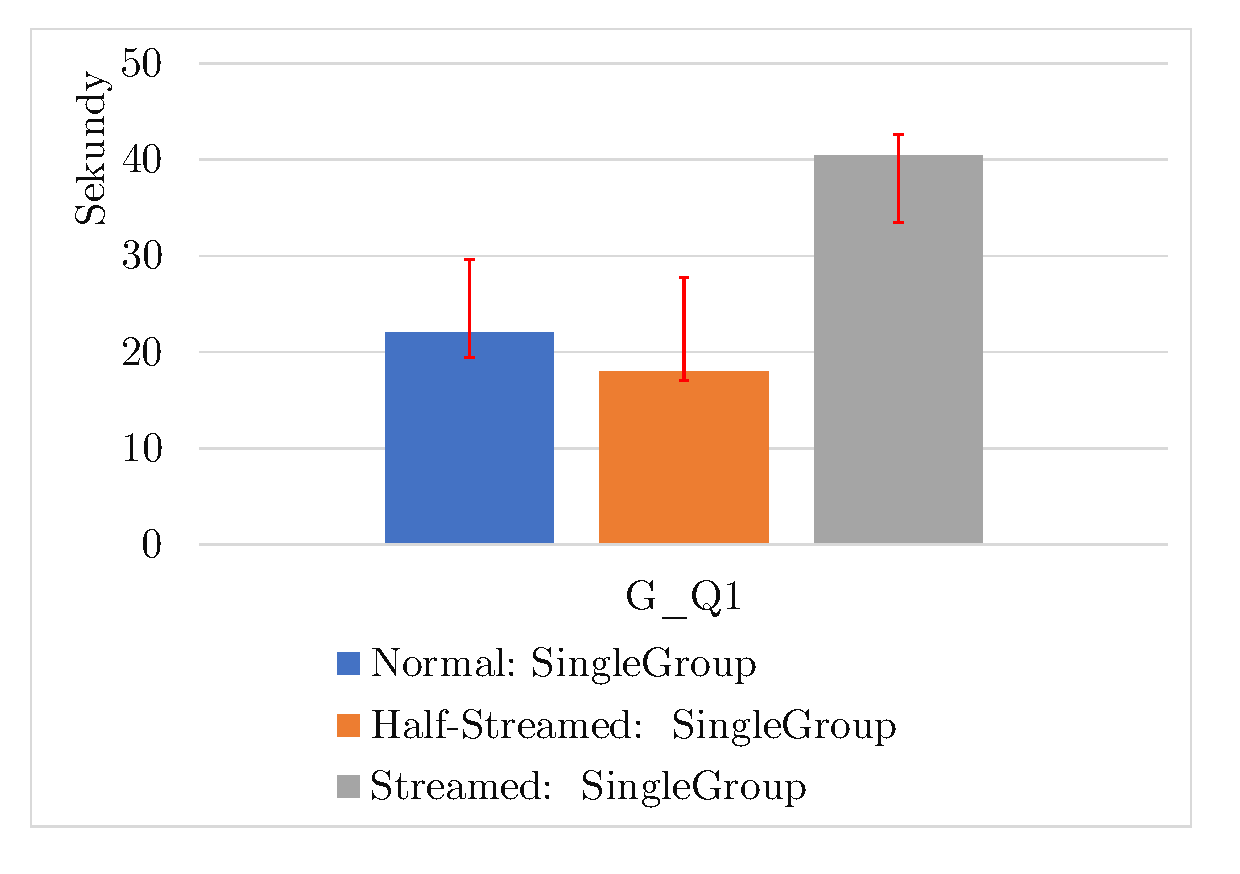
\includegraphics[width=0.9\textwidth]{../img/skitterGroupByQ1Par.pdf} % second figure itself
        \caption{Doba vykonání dotazu G\_Q1 pro graf As-Skitter (sekce \ref{tab.grafBase}). Běh osmi vláken.}
        \label{figure.skitterGQ1Par}
    \end{minipage}
\end{figure}

\subsubsection{Výsledky Single group Group by zpracování}

Na obrázcích \ref{figure.amazonGQ1ST} až \ref{figure.skitterGQ1Par} lze vidět značnou konzistenci mezi výsledky testování při nárustu počtu výsledků vyhledávání.
\textbf{Half-Streamed} a \textbf{Streamed} řešení zde neukládá výsledky vyhledávání do tabulky, ale pouze na aktuální výsledek aplikuje agregační funkce a následně jej zahodí.
To způsobuje značnou výhodu oproti \textbf{Normal} řešení, které drží všechny výsledky v paměti.
Použijeme-li poznatky z sekce \ref{matchResults} o zpomalení způsobeném ukládáním výsledků do tabulky zjistíme (v našem případě jedné proměnné), že rozdíl mezi \textbf{Normal} a \textbf{Half-Streamed} řešením se pohybuje právě v rozsahu onoho zpomalení.
To platí pro běh jednoho vlákna i běhu osmi vláken. 
Problem představuje paralelní \textbf{Streamed} řešení, jelikož k jednomu výsledku přistupuje osm vláken najednou, což způsobuje značné zpomalení kvůli nutné synchronizaci při výpočtu funkcí \verb+min+ a \verb+avg+. 
Zrychlení je zde pouze v rozsahu $[1,81; 2,64]$-krát, zatímco u zbylých řešení je $[3,67; 4,61]$-krát.

Tímto jsme zakončili prezentaci výsledků. 
Všechna nasbíraná data použitá k tvorbě grafů je možné nalézt v příloze výsledků benchmarku (\ref{prilohy.grafyVysledky}). 
